%% abtex2-modelo-trabalho-academico.tex, v-1.9.6 laurocesar
%% Copyright 2012-2016 by abnTeX2 group at http://www.abntex.net.br/ 
%%
%% This work may be distributed and/or modified under the
%% conditions of the LaTeX Project Public License, either version 1.3
%% of this license or (at your option) any later version.
%% The latest version of this license is in
%%   http://www.latex-project.org/lppl.txt
%% and version 1.3 or later is part of all distributions of LaTeX
%% version 2005/12/01 or later.
%%
%% This work has the L PPL maintenance status `maintained'.
%% 
%% The Current Maintainer of this work is the abnTeX2 team, led
%% by Lauro César Araujo. Further information are available on 
%% http://www.abntex.net.br/
%%
%% This work consists of the files abntex2-modelo-trabalho-academico.tex,
%% abntex2-modelo-include-comandos and abntex2-modelo-references.bib
% ------------------------------------------------------------------------
% ------------------------------------------------------------------------
% abnTeX2: Modelo de Trabalho Academico (tese de doutorado, dissertacao de
% mestrado e trabalhos monograficos em geral) em conformidade com 
% ABNT NBR 14724:2011: Informacao e documentacao - Trabalhos academicos -
% Apresentacao
% ------------------------------------------------------------------------
% ------------------------------------------------------------------------
% Personalização para o modelo Udesc 2020 7. ed. revisada e modificada
% MANUAL_2020_09_07_1599489825065_12510.pdf
% Autor: Felipe Joel Zimann (felipezimann@hotmail.com)
% Data: 02/12/2020 v1.0
% Data: 13/02/2021 v1.0.1 alterado tamanho numeração da página para 10pt
% ------------------------------------------------------------------------
% ------------------------------------------------------------------------

\documentclass[
	12pt,					% tamanho da fonte
	openright,				% capítulos começam em pág ímpar (insere página vazia caso preciso)
	oneside,				% para impressão em recto e verso (twoside). Oposto a (oneside)
	a4paper,				% tamanho do papel. 
	chapter=TITLE,			% títulos de capítulos convertidos em letras maiúsculas
	section=TITLE,			% títulos de seções convertidos em letras maiúsculas
	sumario=abnt-6027-2012,
	english,				% idioma adicional para hifenização
	brazil,					% o último idioma é o principal do documento
	fleqn,					% equações alinhadas a esquerda (UDESC/CCT)+
	]{abntex2}

% ----------------------------------------------------------
% Pacotes básicos 
% ----------------------------------------------------------
\usepackage{amsmath}							% Pacote matemático
\usepackage{amssymb}							% Pacote matemático
\usepackage{amsfonts}							% Pacote matemático
%\usepackage{lmodern}							% Usa a fonte Latin Modern		
\usepackage{mathptmx} 							% Usa a fonte Times New Roman	 (UDESC/CCT)
\usepackage[T1]{fontenc}						% Selecao de codigos de fonte.
\usepackage[utf8]{inputenc}						% Codificacao do documento (conversão automática dos acentos)
\usepackage{lastpage}							% Usado pela Ficha catalográfica
\usepackage{indentfirst}						% Indenta o primeiro parágrafo de cada seção.
\usepackage[dvipsnames,table]{xcolor}			% Controle das cores
\usepackage{graphicx}							% Inclusão de gráficos
\usepackage{microtype} 							% para melhorias de justificação
\usepackage{lipsum}								% para geração de dummy text
\usepackage[brazilian,hyperpageref]{backref}	% Paginas com as citações na bibl
\usepackage[alf,abnt-emphasize=bf,abnt-full-initials=yes]{abntex2cite}					% Citações padrão ABNT
%\usepackage[num]{abntex2cite}					% Citações padrão ABNT numérica
\usepackage{adjustbox}							% Pacote de ajuste de boxes
\usepackage{subcaption}							% Inclusão de Subfiguras e sublegendas		
\usepackage{enumitem}							% Personalização de listas
\usepackage{siunitx}							% Grandezas e unidades
\usepackage[section]{placeins}					% Manter as figuras delimitadas na respectiva seção com a opção [section]
\usepackage{multirow}							% Multi colunas nas tabelas
\usepackage{array,tabularx} 					% Pacotes de tabelas
\usepackage{booktabs}							% Pacote de tabela profissonal
\usepackage{rotating}							% Rotacionar figuras e tabelas
\usepackage{xfrac}								% Fazer frações n/d em linha
\usepackage{bm}									% Negrito em modo matemático
\usepackage{xstring}							% Manipulação de strings
\usepackage{pgfplots}							% Pacote de Gráficos
\usepackage{tikz}								% Pacote de Figuras
\usepackage{acronym}
\usepackage[american, cuteinductors,smartlabels, fulldiode, siunitx, americanvoltages, oldvoltagedirection, smartlabels]{circuitikz}						% Pacote de circuitos elétricos
\usepackage{chemformula}						% Pacote para fórmulas químicas
\usepackage{chngcntr}							% Pacte usado para deixar numeração de equações sequencial (UDESC/CCT)
\counterwithout{equation}{chapter}
% fonte: https://latex.org/forum/viewtopic.php?t=15392

% Comando para deixar numeração das equações contínua (1), (2), (3)... ao invés de organizar por capítulos (1.1)(1.2)... (2.1)(2.2)
%\renewcommand{\theequation}{\arabic{equation}}

%\numberwithin{equation}{section}


% Cabecalho cabeçalho somente com numeração de página 10pt
\makepagestyle{PagNumReduzida}
\makeevenhead{PagNumReduzida}{\ABNTEXfontereduzida\thepage}{}{}
\makeoddhead{PagNumReduzida}{}{}{\ABNTEXfontereduzida\thepage}
%fonte: https://github.com/abntex/abntex2/wiki/HowToCustomizarCabecalhoRodape
%fonte: Manual memoir seção 7.3 pg. 111 pdf http://linorg.usp.br/CTAN/macros/latex/contrib/memoir/memman.pdf 

% Personalização das opções das listas
\setlist[itemize]{leftmargin=\parindent}

% Citação online --- MODIFICAR ---
\newcommand{\citeshort}[1]{\citeauthoronline{#1}~(\citeyear{#1})}

\newcommand{\me}[1]{Elaborado pelo autor (#1).}

% Configuração do pgfplots
\pgfplotsset{compat=newest} %compat=1.14
\pgfplotsset{plot coordinates/math parser=false} 
\newlength\figureheight 
\newlength\figurewidth 

% Libraries do TiKz
\usetikzlibrary{quotes,angles,arrows}
\usetikzlibrary{through,calc,math}
\usetikzlibrary{graphs,backgrounds,fit}
\usetikzlibrary{shapes,positioning,patterns,shadows}
\usetikzlibrary{decorations.pathreplacing}
\usetikzlibrary{shapes.geometric}
\usetikzlibrary{arrows.meta}
\usetikzlibrary{external}

%\tikzexternalize[]
%\tikzexternalenable
%\tikzexternalize
%\tikzexternaldisable
%\tikzset{external/force remake}
%\tikzexternalize[shell escape=-enable-write18]

% Configurações do CircuiTiKz
\ctikzset{bipoles/thickness=1}
%\ctikzset{bipoles/length=1.2cm}
\ctikzset{monopoles/ground/width/.initial=.2}
\ctikzset{bipoles/resistor/height=0.25}
\ctikzset{bipoles/resistor/width=0.6}
\ctikzset{bipoles/capacitor/height=0.5}
\ctikzset{bipoles/capacitor/width=0.15}
\ctikzset{bipoles/generic/height=0.25}
\ctikzset{bipoles/generic/width=0.6}
%\ctikzset{bipoles/capacitor polar/length=0.5}
%\ctikzset{bipoles/diode/height=.375}
%\ctikzset{bipoles/diode/width=.3}
%\ctikzset{tripoles/thyristor/height=.8}
%\ctikzset{tripoles/thyristor/width=1}
\ctikzset{bipoles/vsourcesin/height=.5}
\ctikzset{bipoles/vsourcesin/width=.5}
\ctikzset{bipoles/cvsourceam/height=.6}
\ctikzset{bipoles/cvsourceam/width=.6}
%\ctikzset{tripoles/european controlled voltage source/width=.4}

\tikzstyle{every node}=[font=\footnotesize]
\tikzstyle{every path}=[line width=0.25pt,line cap=round,line join=round]
%\tikzstyle{every path}=[line cap=round,line join=round]


% Definição de cores MATLAB
\definecolor{matlab_blue}{rgb}	{         0,    0.4470,    0.7410}
\definecolor{matlab_orange}{rgb}{    0.8500,    0.3250,    0.0980}
\definecolor{matlab_yellow}{rgb}{    0.9290,    0.6940,    0.1250}
\definecolor{matlab_violet}{rgb}{    0.4940,    0.1840,    0.5560}
\definecolor{matlab_green}{rgb}	{	 0.4660,    0.6740,    0.1880}
\definecolor{matlab_lblue}{rgb}	{    0.3010,    0.7450,    0.9330}
\definecolor{matlab_red}{rgb}	{    0.6350,    0.0780,    0.1840}

% Personalização das legendas
\usepackage[format = plain, %hang
			justification = centering,
			labelsep = endash,
			singlelinecheck = false,
			skip = 6pt,
			listformat = simple]{caption}	

% Personalização das unidades
\sisetup{output-decimal-marker = {,}}
\sisetup{exponent-product = \cdot}%, output-product = \cdot}
\sisetup{tight-spacing=true}
\sisetup{group-digits = false}

\usepackage{xcolor}

% Personalizações de tipo de colunas de tabelas
\newcolumntype{L}[1]{>{\raggedright\let\newline\\\arraybackslash\hspace{0pt}}m{#1}}
\newcolumntype{C}[1]{>{\centering\let\newline\\\arraybackslash\hspace{0pt}}m{#1}}
\newcolumntype{R}[1]{>{\raggedleft\let\newline\\\arraybackslash\hspace{0pt}}m{#1}}

% Personalizações de cores da UDESC
\definecolor{CapaAmareloUDESC}{RGB}{243,186,83}		% Especializacao
\definecolor{CapaVerdeUDESC}{RGB}{0,112,52}			% Mestrado
\definecolor{CapaVermelhoUDESC}{RGB}{171,35,21}		% Doutorado
\definecolor{CapaAzulUDESC}{RGB}{38,54,118} 		% Pós-Doutorado

% CONFIGURAÇÕES DE PACOTES
% Configurações do pacote backref
% Usado sem a opção hyperpageref de backref
\renewcommand{\backrefpagesname}{Citado na(s) página(s):~}
% Texto padrão antes do número das páginas
\renewcommand{\backref}{}
% Define os textos da citação
\renewcommand*{\backrefalt}[4]{
	\ifcase #1 %
	Nenhuma citação no texto.%
	\or
	Citado na página #2.%
	\else
	Citado #1 vezes nas páginas #2.%
	\fi}%

% alterando o aspecto da cor azul
%\definecolor{blue}{RGB}{41,5,195}

% informações do PDF
\makeatletter
\hypersetup{
	%pagebackref=true,
	pdftitle={\@title}, 
	pdfauthor={\@author},
	pdfsubject={\imprimirpreambulo},
	pdfcreator={LaTeX with abnTeX2},
	pdfkeywords={abnt}{latex}{abntex}{abntex2}{trabalho academico}, 
	colorlinks=true,       		% false: boxed links; true: colored links
	linkcolor=black,          	% color of internal links
	citecolor=black,        	% color of links to bibliography
	filecolor=black,      		% color of file links
	urlcolor=black,
	bookmarksdepth=4
}
\makeatother


\makeatletter
\newcommand{\includetikz}[1]{%
	\tikzsetnextfilename{#1}%
	\input{#1.tex}%
}
\makeatother

% ---
% Possibilita criação de Quadros e Lista de quadros.
% Ver https://github.com/abntex/abntex2/issues/176
%
\newcommand{\quadroname}{Quadro}
\newcommand{\listofquadrosname}{Lista de quadros}

\newfloat[chapter]{quadro}{loq}{\quadroname}
\newlistof{listofquadros}{loq}{\listofquadrosname}
\newlistentry{quadro}{loq}{0}

% configurações para atender às regras da ABNT
\setfloatadjustment{quadro}{\centering}
\counterwithout{quadro}{chapter}
\renewcommand{\cftquadroname}{\quadroname\space} 
\renewcommand*{\cftquadroaftersnum}{\hfill--\hfill}

\setfloatlocations{quadro}{hbtp} % Ver https://github.com/abntex/abntex2/issues/176
% ---


% Espaçamento depois do título
\setlength{\afterchapskip}{0.7\baselineskip}
% O tamanho do parágrafo é dado por:
\setlength{\parindent}{1.25cm}
% Controle do espaçamento entre um parágrafo e outro:
\setlength{\parskip}{0.0cm}  % tente também \onelineskip
%\SingleSpacing % Espaçamento simples 
\OnehalfSpacing % Espaçamento 1,5 (UDESC/CCT)
%\DoubleSpacing	% Espaçamento duplo

% ---
% Margens - NBR 14724/2011 - 5.1 Formato
% ---
\setlrmarginsandblock{3cm}{2cm}{*}
\setulmarginsandblock{3cm}{2cm}{*}
\checkandfixthelayout[fixed]
% ---


% To use externalize consider
%https://tex.stackexchange.com/questions/182783/tikzexternalize-not-compatible-with-miktex-2-9-abntex2-package
%Lauro Cesar digged into the problem until he came with a solution for me to test. And it Works!
%
%According to this link:
%
%The package calc changed the commands \setcounter and friends to be fragile. So you have to make them robust. The example below uses etoolbox with \robustify:
%
\usepackage{etoolbox}
\robustify\setcounter
\robustify\addtocounter
\robustify\setlength
\robustify\addtolength


%% How to silence memoir class warning against the use of caption package?
%% https://tex.stackexchange.com/questions/391993/how-to-silence-memoir-class-warning-against-the-use-of-caption-package
%\usepackage{silence}
%\WarningFilter*{memoir}{You are using the caption package with the memoir class}
%\WarningFilter*{Class memoir Warning}{You are using the caption package with the memoir class}

% --------------------------------------------------------
% INICIO DAS CUSTOMIZACOES PARA A UDESC
% --------------------------------------------------------

% --------------------------------------------------------
% Fontes padroes de part, chapter, section, subsection e subsubsection
% --------------------------------------------------------
% --- Chapter ---
\renewcommand{\ABNTEXchapterfont}{\fontseries{b}} %\bfseries
\renewcommand{\ABNTEXchapterfontsize}{\normalsize}
% --- Part ---
\renewcommand{\ABNTEXpartfont}{\ABNTEXchapterfont}
\renewcommand{\ABNTEXpartfontsize}{\LARGE}
% --- Section ---
\renewcommand{\ABNTEXsectionfont}{\normalfont}
\renewcommand{\ABNTEXsectionfontsize}{\normalsize}
% --- SubSection ---
\renewcommand{\ABNTEXsubsectionfont}{\fontseries{b}} %\bfseries
\renewcommand{\ABNTEXsubsectionfontsize}{\normalsize}
% --- SubSubSection ---
\renewcommand{\ABNTEXsubsubsectionfont}{\itshape}
\renewcommand{\ABNTEXsubsubsectionfontsize}{\normalsize}

\renewcommand{\ABNTEXsubsubsubsectionfont}{\normalfont}
\renewcommand{\ABNTEXsubsubsubsectionfontsize}{\normalsize}
% ---

% --------------------------------------------------------
% Fontes das entradas do sumario
% --------------------------------------------------------

\renewcommand{\cftpartfont}{\ABNTEXpartfont\selectfont}
\renewcommand{\cftpartpagefont}{\normalsize\selectfont}

\renewcommand{\cftchapterfont}{\ABNTEXchapterfont\selectfont}
\renewcommand{\cftchapterpagefont}{\normalsize\selectfont}

\renewcommand{\cftsectionfont}{\ABNTEXsectionfont\selectfont}
\renewcommand{\cftsectionpagefont}{\normalsize\selectfont}

\renewcommand{\cftsubsectionfont}{\ABNTEXsubsectionfont\selectfont}
\renewcommand{\cftsubsectionpagefont}{\normalsize\selectfont}

\renewcommand{\cftsubsubsectionfont}{\normalfont\itshape\selectfont}
\renewcommand{\cftsubsubsectionpagefont}{\normalsize\selectfont}

\renewcommand{\cftparagraphfont}{\normalfont\selectfont}
\renewcommand{\cftparagraphpagefont}{\normalsize\selectfont}

% --------------------------------------------------------
% Usando os pacotes hyperref, uppercase... 
% Para deixar a section do toc uppercase precisa de:
% --------------------------------------------------------
\usepackage{textcase}

\makeatletter

\let\oldcontentsline\contentsline
\def\contentsline#1#2{%
	\expandafter\ifx\csname l@#1\endcsname\l@section
	\expandafter\@firstoftwo
	\else
	\expandafter\@secondoftwo
	\fi
	{%
		\oldcontentsline{#1}{\MakeTextUppercase{#2}}%
	}{%
		\oldcontentsline{#1}{#2}%
	}%
}
\makeatother

% --------------------------------------------------------
% Renomenando as entradas de APÊNDICES E ANEXOS
% --------------------------------------------------------

\renewcommand{\apendicesname}{AP\^ENDICES}
\renewcommand{\anexosname}{ANEXOS}


% Manipulação de Strings
%\RequirePackage{xstring}

% Comando para inverter sobrenome e nome
\newcommand{\invertname}[1]{%
	\StrBehind{#1}{{}}, \StrBefore{#1}{{}}%
}%


% --------------------------------------------------------
% Alterando os estilos de Caption e Fonte
% --------------------------------------------------------
\makeatletter
% Define o comando \fonte que respeita as configurações de caption do memoir ou do caption
\renewcommand{\fonte}[2][\fontename]{%
	\M@gettitle{#2}%
	\memlegendinfo{#2}%
	\par
	\begingroup
	\@parboxrestore
	\if@minipage
	\@setminipage
	\fi
	\ABNTEXfontereduzida
	\configureseparator
	\captiondelim{\ABNTEXcaptionfontedelim}
	\@makecaption{#1}{\ignorespaces #2}\par
	\endgroup}


\captionstyle[\raggedright]{\raggedright}

\makeatother

\setlength{\cftbeforechapterskip}{0pt plus 0pt}
\renewcommand*{\insertchapterspace}{}

\newlength{\mylen}	% New length to use with spacing
\setlength{\mylen}{1pt}

\setlength{\cftbeforechapterskip}{\mylen}
\setlength{\cftbeforesectionskip}{\mylen}
\setlength{\cftbeforesubsectionskip}{\mylen}
\setlength{\cftbeforesubsubsectionskip}{\mylen}
\setlength{\cftbeforesubsubsubsectionskip}{\mylen}


% ---
% Ajuste das listas de abreviaturas e siglas ; e símbolos [Personalizada para UDESC com espaçamento 1,5]
% ---

% ---
% Redefinição da Lista de abreviaturas e siglas [Personalizada para UDESC com espaçamento 1,5]
\renewenvironment{siglas}{%
	\pretextualchapter{\listadesiglasname}
	\begin{symbols} 
		\setlength{\itemsep}{0pt}	% Ajuste para Espaçamento 1,5 (UDESC/CCT)
	}{% 
	\end{symbols}
	\cleardoublepage
}
% ---

% ---
% Redefinição da Lista de símbolos [Personalizada para UDESC com espaçamento 1,5]
\renewenvironment{simbolos}{%
	\pretextualchapter{\listadesimbolosname}
	\begin{symbols}
		\setlength{\itemsep}{0pt}	% Ajuste para Espaçamento 1,5 (UDESC/CCT)
	}{%
	\end{symbols}
	\cleardoublepage
}
% ---





% ---
% FIM DAS CUSTOMIZACOES PARA A  Universidade do Estado de Santa Catarina - UDESC/CCT
% ---





	% Incliu pacotes básicos 

% -----------------------------------------------------------------
% Você pode adicionar seus pacotes a partir desta linha;
% -----------------------------------------------------------------

%\usepackage[showframe,pass]{geometry}
%\usepackage[11,12]{pagesel}

\renewcommand{\orientadorname}{Orientadora:}
\renewcommand{\coorientadorname}{Coorientadora:}

% -----------------------------------------------------------------
% Informações de dados para CAPA e FOLHA DE ROSTO
% -----------------------------------------------------------------

\titulo{Detecção de padrões em relação à presença dos estudantes no ensino básico brasileiro}%

\autor{Daniella {}Martins Vasconcellos}%
\orientador{Isabela {}Gasparini}%
\coorientador{Elaine Harada {}Teixeira de Oliveira}%

% ATENÇÃO: O símbolo {} indica o sobrenome para a ficha catalográfica.
% Exemplo: Sherlock Holmes {}da Silva para sobrenomes compostos;
% Exemplo: Arnold Alois {}Schwarzenegger para sobrenome simples.

\instituicao{Universidade do Estado de Santa Catarina, Centro de Ciências Tecnológicas, Programa de Graduação em Ciência da Computação}%

%\tipotrabalho{Tese (Doutorado)}
\tipotrabalho{Trabalho de Conclusão de Curso}

%\preambulo{Tese apresentada ao Programa de Pós--Graduação em Engenharia Elétrica do Centro de Ciências Tecnológicas da Universidade do Estado de Santa Catarina, como requisito parcial para a obtenção do grau de Doutor em Engenharia Elétrica.}

\preambulo{Trabalho de Conclusão de Curso I submetido à
Universidade do Estado de Santa Catarina como
parte dos requisitos para a obtenção do grau de
Bacharel em Ciência da Computação}

\local{Joinville}%

\data{\the\year}%
% ---

% compila o indice
\makeindex

% -----------------------------------------------------------------
% Início do documento
% -----------------------------------------------------------------
\begin{document}

\selectlanguage{brazil}
\frenchspacing  % Retira espaço extra obsoleto entre as frases.

% -----------------------------------------------------------------
% ELEMENTOS PRÉ-TEXTUAIS
% -----------------------------------------------------------------
\pretextual

% Você pode comentar os elementos que não deseja em seu trabalho;

% A capa pode ser escolhida dentro do arquivo Capa.tex (TCC, Master, Doc, ...)
% ---
% Capa
% ---


% --------------------------------------------------------
% Capa Padrão
% --------------------------------------------------------
\renewcommand{\imprimircapa}{%
	\begin{capa}%
		\center

		{\fontseries{b}\selectfont\MakeTextUppercase{UNIVERSIDADE DO ESTADO DE SANTA CATARINA -- UDESC}}
		
		{\fontseries{b}\selectfont\MakeTextUppercase{CENTRO DE CIÊNCIAS TECNOLÓGICAS -- CCT  }}
		
		{\fontseries{b}\selectfont\MakeTextUppercase{TRABALHO DE CONCLUSÃO DE CURSO -- CIÊNCIA DA COMPUTAÇÃO  }}
		
		\vfill
		
		{\fontseries{b}\selectfont\MakeTextUppercase{\normalsize Daniella Martins Vasconcellos}}
		
		\vfill
		\begin{center}
			{\fontseries{b}\selectfont\MakeTextUppercase{Detecção de padrões em relação à presença dos estudantes no ensino básico brasileiro}}
		\end{center}
		\vfill
		
		\vfill
		
		{\fontseries{b}\selectfont\MakeTextUppercase{\imprimirlocal}}
		\par
		{\fontseries{b}\selectfont \imprimirdata}
		\vspace*{1cm}
	\end{capa}
}



\imprimircapa				% Capa padrão

					% Elemento Obrigatório
% ---
% Folha de rosto
% ---








% --------------------------------------------------------
% folha de rosto 
% --------------------------------------------------------

\makeatletter

\renewcommand{\folhaderostocontent}{
	\begin{center}
		
		{\fontseries{b}\selectfont\MakeTextUppercase{\imprimirautor}}
		
		\vfill
		
		\begin{center}
			{\fontseries{b}\selectfont\MakeTextUppercase{\imprimirtitulo}}
		\end{center}
	
		\vspace*{1.5cm}

		\abntex@ifnotempty{\imprimirpreambulo}{%
			\hspace{.45\textwidth}
			{\begin{minipage}{.5\textwidth}
					\SingleSpacing
					\imprimirpreambulo\par
					\vspace*{4pt}
					{\imprimirorientadorRotulo~\imprimirorientador\par}
					\abntex@ifnotempty{\imprimircoorientador}{%
						{\imprimircoorientadorRotulo~\imprimircoorientador \space (UFAM)}%
					}%
			\end{minipage}}%
		}%
	
		
		\vfill
		
	{\fontseries{b}\selectfont\MakeTextUppercase{\imprimirlocal}}
	\par
	{\fontseries{b}\selectfont \imprimirdata}
	\vspace*{1cm}
	\end{center}
}


% (o * indica que haverá a ficha bibliográfica)
% ---
\imprimirfolhaderosto*
% ---


			% Elemento Obrigatório
% Caso não utilize a Ficha Catalográfica entre na folha de rosto e retire o * de dentro do arquivo FolhadeRosto

% ---
% Inserir a ficha bibliografica
% ---

% Isto é um exemplo de Ficha Catalográfica, ou ``Dados internacionais de
% catalogação-na-publicação''. Você pode utilizar este modelo como referência. 
% Porém, provavelmente a biblioteca da sua universidade lhe fornecerá um PDF
% com a ficha catalográfica definitiva após a defesa do trabalho. Quando estiver
% com o documento, salve-o como PDF no diretório do seu projeto e substitua todo
% o conteúdo de implementação deste arquivo pelo comando abaixo:



% \begin{fichacatalografica}
%     \includepdf{fig_ficha_catalografica.pdf}
% \end{fichacatalografica}


%	\setlength{\parindent}{0cm}
%	\setlength{\parskip}{0pt}
\begin{fichacatalografica}
	%\sffamily
	%\rmfamily
	\ttfamily \hbadness=10000
	\vspace*{\fill}					% Posição vertical
	\begin{center}					% Minipage Centralizado
	Para gerar a ficha catalográfica de teses e \\ 
	dissertações acessar o link:  \\
	https://www.udesc.br/bu/manuais/ficha
	
	\vspace*{8pt}
	
%	\begin{minipage}[c]{8cm}
%	\centering \sffamily
%	 Ficha catalográfica elaborada pelo(a) autor(a), com auxílio do programa de geração automática da Biblioteca Setorial do CCT/UDESC
%	\end{minipage}
	\fbox{\begin{minipage}[c]{12.5cm}		% Largura
	\flushright
	{\begin{minipage}[c]{10.5cm}		% Largura
	\vspace{1.25cm}
	%\footnotesize
	\setlength{\parindent}{1.5em}
	\noindent \invertname{\imprimirautor} \par
	\imprimirtitulo{ }/{ }\imprimirautor. -- \imprimirlocal, \imprimirdata .\par
	\pageref{LastPage} p. : il. ; 30 cm.\par
	\vspace{1.5em}
	\imprimirorientadorRotulo~\imprimirorientador.\par
	\imprimircoorientadorRotulo~\imprimircoorientador.\par
	\imprimirtipotrabalho~--~\imprimirinstituicao, \imprimirlocal, \imprimirdata.\par
	\vspace{1.5em}
		1. Mineração de dados educacionais.
 		2. Análise classificatória.
		3. Evasão.
		I. \invertname{\imprimirorientador}.
		II. \invertname{\imprimircoorientador}.
		III. \imprimirinstituicao.
		IV. Detecção de padrões em relação à presença dos estudantes no ensino básico brasileiro. %
	\vspace{1.25cm}	%		
	\end{minipage}%
	}% 
	\end{minipage}}%
	
	\vspace*{0.5cm}
	
	\end{center}
\end{fichacatalografica}


%\begin{fichacatalografica}
%	\sffamily
%	\vspace*{\fill}					% Posição vertical
%	\begin{center}					% Minipage Centralizado
%	\fbox{\begin{minipage}[c][8cm]{13.5cm}		% Largura
%	\small
%	\imprimirautor
%	%Sobrenome, Nome do autor
%	
%	\hspace{0.5cm} \imprimirtitulo  / \imprimirautor. --
%	\imprimirlocal, \imprimirdata-
%	
%	\hspace{0.5cm} \pageref{LastPage} p. : il. (algumas color.) ; 30 cm.\\
%	
%	\hspace{0.5cm} \imprimirorientadorRotulo~\imprimirorientador\\
%	
%	\hspace{0.5cm}
%	\parbox[t]{\textwidth}{\imprimirtipotrabalho~--~\imprimirinstituicao,
%	\imprimirdata.}\\
%	
%	\hspace{0.5cm}
%		1. Palavra-chave1.
%		2. Palavra-chave2.
%		3. Palavra-chave3.
% 		4. Palavra-chave4.
%		5. Palavra-chave5.
%		I. Orientador.
%		II. Universidade xxx.
%		III. Faculdade de xxx.
%		IV. Título 			
%	\end{minipage}}
%	\end{center}
%\end{fichacatalografica}
% ---

	% Elemento Obrigatório (Verso da Folha)

% % ---
% % Inserir errata
% % ---
% \begin{errata}
% Elemento opcional. 

% Exemplo:

% \vspace{\onelineskip}

% SOBRENOME, Prenome do Autor. Título de obra: subtítulo (se houver). Ano de depósito. Tipo do trabalho (grau e curso) - Vinculação acadêmica, local de apresentação/defesa, data.

% \begin{table}[htb]
% \center
% \begin{tabular}{|p{2.4cm}|p{2cm}|p{3cm}|p{3cm}|}
%   \hline
%    \textbf{Folha} & \textbf{Linha}  & \textbf{Onde se lê}  & \textbf{Leia-se}  \\
%     \hline
%     1 & 10 & auto-conclavo & autoconclavo\\
%    \hline
% \end{tabular}
% \end{table}

% \end{errata}
% % ---				% Elemento Opcional

% ---
% Inserir folha de aprovação
% ---

% Isto é um exemplo de Folha de aprovação, elemento obrigatório da NBR
% 14724/2011 (seção 4.2.1.3). Você pode utilizar este modelo até a aprovação
% do trabalho. Após isso, substitua todo o conteúdo deste arquivo por uma
% imagem da página assinada pela banca com o comando abaixo:
%
% \includepdf{folhadeaprovacao_final.pdf}
%
\begin{folhadeaprovacao}



	\begin{center}
		{\fontseries{b}\selectfont\MakeTextUppercase{\normalsize\imprimirautor}}
	\end{center}
    \vfill
    
	\vfill
	\begin{center}
		{\fontseries{b}\selectfont\MakeTextUppercase{\imprimirtitulo}}
	\end{center}
	\vfill

    
\abntex@ifnotempty{\imprimirpreambulo}{%
	\hspace{.45\textwidth}
	{\begin{minipage}{.5\textwidth}
			\SingleSpacing
			\imprimirpreambulo\par
			\vspace*{4pt}
			{\imprimirorientadorRotulo~\imprimirorientador\par}
			\abntex@ifnotempty{\imprimircoorientador}{%
				{\imprimircoorientadorRotulo~\imprimircoorientador \space (UFAM)}%
			}%
	\end{minipage}}%
}%


\vfill
        
	 \begin{center}
	 	
    	{\fontseries{b}\selectfont BANCA EXAMINADORA: }
    	\vspace*{1.75cm}
    
		  Isabela Gasparini -- Doutorado em Computação \par
		Universidade do Estado de Santa Catarina
	 \end{center}
	
    {Membros:} 
    
	\begin{center}
        \vspace*{1.25cm}
		Elaine Harada Teixeira de Oliveira -- Doutorado em Informática na Educação\par
		Universidade Federal do Amazonas
  
		\vspace*{1.25cm}
		Debora Cabral Nazario -- Doutorado em Engenharia e Gestão do Conhecimento \par
		Universidade do Estado de Santa Catarina
		
		\vspace*{1.25cm}
		Rebeca Schroeder Freitas -- Doutorado em Informática \par
		Universidade do Estado de Santa Catarina

	
	\end{center}
    
    \vspace*{\fill}  
    \begin{center}
        {\imprimirlocal, \today} %\imprimirdata}
	\end{center}
    \vspace*{0.25cm}  
\end{folhadeaprovacao}
% ---




%\textbf{	{Orientador: \vspace{-16pt} }
%	\assinatura{\textbf{Prof. \imprimirorientador , Dr.} \\ Univ. XXX} 
%	{Coorientador: \vspace{-16pt}}   
%	\assinatura{\textbf{Prof. \imprimircoorientador , Dr.} \\ Univ. XXX}
%	
%	{Membros: \vspace{-16pt} } 
%	
%	% --- Exemplo de assinaturas em sequência ---       
%	\setlength{\ABNTEXsignwidth}{8.5cm}
%	
%	\assinatura{\textbf{Prof. Professor, Dr.} \\ Univ. XXX}
%	\assinatura{\textbf{Prof. Professor, Dr.} \\ Univ. XXX}
%	\assinatura{\textbf{Prof. Professor, Dr.} \\ Univ. XXX}
%	
%	% --- Exemplo de assinaturas lado a lado ---
%	\setlength{\ABNTEXsignwidth}{7.5cm}
	%
	%    \noindent\hfill\assinatura*{\textbf{Prof. Professor, Dr.} \\ Univ. XXX}%
	%    \hfill%
	%    \assinatura*{\textbf{Prof. Professor, Dr.} \\ Univ. XXX}%
	%    \hfill
	%    
	%    \noindent\hfill\assinatura*{\textbf{Prof. Professor, Dr.} \\ Univ. XXX}%
	%    \hfill%
	%    \assinatura*{\textbf{Prof. Professor, Dr.} \\ Univ. XXX}%
	%    \hfill}		% Elemento Obrigatório
% ---
% Dedicatória
% ---
\begin{dedicatoria}
   \vspace*{\fill}
%   \begin{flushright}
%   \noindent
%	Este trabalho é dedicado às crianças adultas que,\\
%	quando pequenas, sonharam em se tornar cientistas. 
%   \end{flushright}

{%
	\noindent\hspace{.5\textwidth}
	{\begin{minipage}{.5\textwidth}
			\begin{flushleft}
				Aos meus amigos, pela inspiração e pela confiança.
			\end{flushleft}
	\end{minipage}}%
\vspace*{3cm}
}%

\end{dedicatoria}
% ---
			% Elemento Opcional
% ---
% Agradecimentos
% ---
\begin{agradecimentos}
Agradeço às minhas orientadoras, Isabela Gasparini e Elaine Harada Teixeira de Oliveira, por aceitarem conduzir o meu trabalho de pesquisa.

Aos meus pais, pelo apoio incondicional frente a tantas dificuldades.

A todos os meus amigos que estiveram ao meu lado durante essa longa trajetória, me dando forças para continuar seguindo em frente.

Ao meu grupo de iniciação científica, Grupo de Pesquisa em Informática na Educação (GPIE), em especial aos colegas também orientados pela professora Isabela Gasparini, conhecidos como Artigos \& Amigos, que tiveram grande impacto na construção da minha produção científica, a qual se inclui esse trabalho de conclusão de curso. %Como disse Ada Lovelace: ``Nunca estou realmente satisfeita quanto a entender alguma coisa; porque, até onde entendo, a minha compreensão só pode ser uma fração infinitesimal de tudo o que eu quero compreender''.

Deixo um agradecimento especial à minha orientadora, Isabela Gasparini, pelo incentivo, pela dedicação do seu escasso tempo ao meu projeto de pesquisa, e principalmente pela confiança que depositou em mim durante os últimos anos; à minha coorientadora, Elaine Harada Teixeira de Oliveira, que conseguiu me manter calma em momentos críticos da finalização desse trabalho; e às minhas amigas Laís Piseta Van Vossen e Maria Teresa Silva Santos por toda a ajuda.


\end{agradecimentos}
% ---		% Elemento Opcional
% ---
% Epígrafe
% ---
\begin{epigrafe}
    \vspace*{\fill}
%	\begin{flushright}
%		\textit{``Eu não falhei, encontrei 10 mil soluções que não davam certo.'' (EDISON, [19--])}
%	\end{flushright}
{%
	\noindent\hspace{.5\textwidth}
	{\begin{minipage}{.5\textwidth}
		\begin{flushright}
			``\textit{I never am really satisfied that I understand anything; because, understand it well as I may, my comprehension can only be an infinitesimal fraction of all I want to understand about the many connections and relations which occur to me, how the matter in question was first thought of or arrived at.}'' (ADA LOVELACE)
		\end{flushright}
	\end{minipage}}%
	\vspace*{3cm}
}%
\end{epigrafe}
% ---				% Elemento Opcional
% ---
% RESUMOS
% ---

% resumo em português
\setlength{\absparsep}{18pt} % ajusta o espaçamento dos parágrafos do resumo
\begin{resumo}


A educação deveria ser uma prioridade no Brasil, e o Ministério da Educação (MEC) vem implementando políticas visando aprimorar o ensino no país. A coleta de dados dos cidadãos que utilizam serviços educacionais é crucial para o gerenciamento eficiente de recursos e atendimento às necessidades da população. Esses dados são amplamente utilizados por pesquisadores para compreender o sistema educacional e desenvolver programas para melhorar a qualidade da educação. A ciência de identificação de padrões é uma abordagem valiosa para analisar esses dados complexos, permitindo previsões precisas e decisões em evidências. Nesse contexto, o objetivo deste estudo é identificar fatores de risco de evasão de estudantes do ensino fundamental aos quais foram aplicados o Instrumento de Avaliação de Risco de Evasão Escolar (IAFREE). Foram feitas análises estatísticas para traçar correlações entre as variáveis estudadas da base resultante do questionário, e análises de classificação com aprendizado de máquina com o objetivo de descobrir os fatores com maior relevância estatística e que apresentam melhor desempenho dentre as métricas utilizadas para comparação dos algoritmos.

%vêm
% vem implementando políticas visando aprimorar o ensino no país. A coleta de dados dos cidadãos que utilizam serviços educacionais é crucial para o gerenciamento eficiente de recursos e atendimento às necessidades da população. Esses dados são amplamente utilizados por pesquisadores para compreender o sistema educacional e desenvolver programas para melhorar a qualidade da educação. A ciência de identificação de padrões é uma abordagem valiosa para analisar esses dados complexos, permitindo previsões precisas e decisões em evidências. Nesse contexto, o objetivo deste estudo é identificar padrões de presença em sala de aula de estudantes do ensino básico no Brasil, abrangendo a pré-escola, ensino fundamental e médio. Usando aprendizado de máquina e análise de séries temporais, serão identificados padrões de frequência escolar ao longo do tempo. Espera-se que essa análise forneça perspectivas sobre fatores relacionados à evasão escolar e contribua para o desenvolvimento de políticas e programas eficazes.

% Elemento obrigatório que contém a apresentação concisa dos pontos relevantes do trabalho, fornecendo uma visão rápida e clara do conteúdo e das conclusões do mesmo. A apresentação e a redação do resumo devem seguir os requisitos estipulados pela NBR 6028 (ABNT, 2003). Deve descrever de forma clara e sintética a natureza do trabalho, o objetivo, o método, os resultados e as conclusões, visando fornecer elementos para o leitor decidir sobre a consulta do trabalho no todo.

 \textbf{Palavras-chave}: Mineração de dados educacionais. Análise classificatória. Machine learning. Evasão.
\end{resumo}
				% Elemento Obrigatório
% ---
% Abstract
% ---

% resumo em inglês
\begin{resumo}[Abstract]
 \begin{otherlanguage*}{english}

Education should be a priority in Brazil, and the Ministry of Education (MEC) has been implementing policies aimed at improving education in the country. The collection of data from citizens using educational services is crucial for efficient resource management and meeting the needs of the population. These data are widely used by researchers to understand the education system and develop programs to enhance the quality of education. The science of pattern identification is a valuable approach for analyzing these complex data, enabling precise predictions and evidence-based decisions. In this context, the objective of this study is to identify risk factors for student dropout in elementary education using the School Dropout Risk Assessment Instrument (IAFREE). Statistical analyses were conducted to establish correlations among the studied variables in the resulting questionnaire dataset, and classification analyses with machine learning were performed to discover the factors with the highest statistical relevance and the best performance among the metrics used for algorithm comparison.
% Education should be a priority in Brazil, and the Ministry of Education (MEC) has been implementing policies to enhance education in the country. The collection of data from citizens who use educational services is crucial for efficient resource management and meeting the population's needs. Researchers widely utilize this data to understand the educational system and develop programs to improve the quality of education. The science of pattern identification is a valuable approach for analyzing these complex data, enabling accurate predictions and informed decision-making. In this context, the objective of this study is to identify patterns of classroom attendance among students in basic education in Brazil, including preschool, elementary, and high school. Using machine learning and time series analysis, patterns of school attendance over time will be identified. It is expected that this analysis will provide insights into factors related to school dropout and contribute to the development of effective policies and programs.

%   Elemento obrigatório para todos os trabalhos de conclusão de curso. Opcional para os demais trabalhos acadêmicos, inclusive para artigo científico. Constitui a versão do resumo em português para um idioma de divulgação internacional. Deve aparecer em página distinta e seguindo a mesma formatação do resumo em português.

   \textbf{Keywords}: Educational data mining. Classificatiory analysis. Dropout.
 \end{otherlanguage*}
\end{resumo}
				% Elemento Obrigatório

% ---
% inserir lista de ilustrações
% ---
\pdfbookmark[0]{\listfigurename}{lof}
\listoffigures*
\cleardoublepage
% ---

% ---
% inserir lista de quadros
% ---
%\pdfbookmark[0]{\listofquadrosname}{loq}
%\listofquadros*
%\cleardoublepage
% ---


% ---
% inserir lista de tabelas
% ---
\pdfbookmark[0]{\listtablename}{lot}
\listoftables*
\cleardoublepage
% ---

% ---
% inserir lista de abreviaturas e siglas
% ---
\begin{siglas}
\item[DM]   Data Mining
\item[EDM]     {Educational Data Mining}
\item[FNDE]    {Fundo Nacional de Desenvolvimento da Educação}
\item[FUNDEB]  {Fundo de Manutenção e Desenvolvimento da Educação Básica}
\item[GPIE]    {Grupo de Pesquisa em Informática na Educação}
\item[LA]      {Learning Analytics}
\item[MEC]     {Ministério da Educação}
\item[LMS]     {Learning Management Systems}
\item[NEES]    {Núcleo de Excelência em Tecnologias Sociais}
\item[PNAE]    {Programa Nacional de Alimentação Escolar}
\item[PNE]     {Plano Nacional de Educação}
\item[ProUni]  {Portal Único de Acesso ao Ensino Superior} 
\item[SAP]     {Sistema de Alerta Preventivo}
\item[STIC]    {Secretaria de Tecnologia da Informação}
\item[TED]     {Termo de Execução Descentralizada}
\item[TCC]     {Trabalho de Conclusão de Curso}
\item[UDESC]   {Universidade do Estado de Santa Catarina}
\item[UFAL]    {Universidade Federal de Alagoas}
\item[UFAM]    {Universidade Federal do Amazonas}
\end{siglas}
% ---

% ---
% inserir lista de símbolos
% ---


% \begin{simbolos}
%   \item[@] Arroba
%   \item[\%] Porcento
%   \item[$^\circ$C] Graus Celsius
%   \item[Ca] Cálcio
% \end{simbolos}

% ---
				% Elemento Opcional
% ---
% inserir o sumario
% ---
\pdfbookmark[0]{\contentsname}{toc}
\tableofcontents*
\cleardoublepage
% ---
				% Elemento Obrigatório

% -----------------------------------------------------------------
% ELEMENTOS TEXTUAIS
% -----------------------------------------------------------------
\textual

\pagestyle{PagNumReduzida}						% Comando para cabeçalho somente com numeração de página 10pt
\aliaspagestyle{chapter}{PagNumReduzida}		% Deixar numeração da primeira página com tamanho igual ao resto da numeração
% ref.: https://groups.google.com/g/abntex2/c/CP7g8ZMgi-c/m/KjfEnn5b9a4J


% ---- Mantenha está estrutura, assim você deixa o trabalho mais organizado -------

\chapter{Introdução}

O sistema educacional brasileiro tem sido alvo de várias políticas públicas nas últimas décadas, visando garantir o acesso, a permanência e a qualidade do ensino em todas as etapas e modalidades de ensino. Entre as políticas mais relevantes estão o Plano Nacional de Educação (PNE) \cite{PNE:2001}, o Fundo de Manutenção e Desenvolvimento da Educação Básica (FUNDEB) \cite{FUNDEB:2020}, e o Programa Nacional de Alimentação Escolar (PNAE) \cite{PNAE:2009}. O Ministério da Educação (MEC) é o órgão responsável por coordenar e executar as políticas públicas voltadas para a educação no país. Em sua história, o ministério tem atuado de forma significativa na definição das políticas educacionais, na formulação de diretrizes curriculares, na elaboração de programas e materiais didáticos, no estabelecimento de critérios de avaliação e na capacitação de professores.

Como os programas governamentais do MEC têm como objetivo o fornecimento de serviços públicos essenciais para atender a variadas necessidades educacionais da população, é fundamental que se colete informações e dados sobre os cidadãos que usufruem dos serviços para melhor utilização de recursos e retorno à população. Por exemplo, o Portal Único de Acesso ao Ensino Superior (ProUni) acessa dados socioeconômicos dos estudantes que estão em bases governamentais para poder analisar possíveis dispensas de apresentação de documentos (como comprovação de renda familiar mensal bruta ou a situação da pessoa com deficiência) \cite{PROUni:2005}. Dentre outras políticas públicas implementadas pelo governo brasileiro que estão ligadas diretamente ao MEC, o Sistema de Alerta Preventivo (SAP), que, de maneira análoga ao ProUni, acessa dados socioeconômicos dos beneficiários por meio de bases governamentais, mas com o objetivo de ajudar a prevenir a evasão e o abandono escolar, identificando alunos em risco de evasão e direcionando atividades mitigatórias para eles. Com o SAP, é possível antecipar ações preventivas de evasão, tornando mais fácil para as escolas e redes de ensino implementarem ações preventivas focalizadas de combate ao abandono escolar \cite{sap}. Essa prática permite a análise criteriosa de dispensas de documentos, como comprovação de renda familiar mensal bruta ou a situação de pessoas com deficiência, contribuindo para uma gestão eficiente do programa. Sabendo que estudos realizados em outros países, como na Guatemala, mostraram que o SAP pode gerar resultados consistentes nas taxas de evasão e abandono, reduzindo a evasão em até 4 pontos percentuais, é possível concluir que o SAP atua como uma ferramenta estratégica, fornecendo informações relevantes para a tomada de decisões e aprimoramento contínuo das políticas públicas educacionais. %Dentre outras políticas públicas implementadas pelo governo brasileiro que estão ligadas diretamente ao MEC, o Bolsa Família \cite{BolsaFamilia2023} se destaca por ser um programa de transferência de renda que tem como objetivo promover a redução da pobreza e da desigualdade social. O programa foi criado em 2004 \cite{BolsaFamilia}, e tem como uma das principais condições para o recebimento do benefício a frequência escolar dos filhos. Ou seja, para receber o benefício, as famílias precisam se comprometer a manter seus filhos na escola e garantir a frequência escolar mínima estabelecida pelo MEC, que varia de acordo com a faixa etária dos alunos. A coleta da frequência escolar é realizada atualmente pelas escolas em que os alunos estão matriculados, e os dados são repassados ao MEC para fins de monitoramento e avaliação do programa através do Sistema Presença~\footnote{https://presenca.mec.gov.br/}. 

% A coleta de dados de frequência escolar do Bolsa Família é importante porque permite ao governo monitorar a frequência dos alunos e garantir que as famílias estejam cumprindo seus compromissos. Além disso, essa coleta de dados é uma ferramenta importante para as escolas, para as secretarias de Educação (estaduais e municipais)  e para o MEC, pois permite a identificação de problemas de abandono escolar e o desenvolvimento de novas políticas públicas baseadas em evidências para reduzi-los. Esses dados também são utilizados para aferir a qualidade do ensino e a efetividade das já existentes políticas públicas voltadas para a educação \cite{santos:2019, Monteiro:2009}. A partir desses dados, o MEC pode identificar regiões do país, estados, cidades e escolas com baixa frequência escolar e direcionar esforços para melhorar a qualidade do ensino nessas áreas.

% Apesar de sua importância, a coleta de dados de frequência escolar do Bolsa Família ainda enfrenta diversos desafios. Dentre os principais se encontram fragilidades no sistema educacional brasileiro, como a dualidade entre escolas públicas e privadas. Escolas particulares tendem a ser mais equipadas, melhor localizadas e ter professores mais preparados se comparadas às escolas públicas. A diferença de estrutura das escolas para coletar e processar os dados, a falta de treinamento dos professores e gestores escolares para lidar com as informações e a falta de recursos financeiros para implementar sistemas de coleta de dados que permitiriam um processo mais ágil e preciso das informações \cite{DutraThom2016}. Para superar essa dificuldade, o MEC tem buscado parcerias com instituições de tecnologia e com governos locais para garantir o acesso à internet e aos equipamentos necessários para a coleta e processamento dos dados.

% Diante desses desafios, o MEC tem adotado medidas para aprimorar a coleta de dados de frequência escolar do Bolsa Família. Entre as iniciativas em andamento estão a implementação de sistemas de coleta de dados mais eficientes e o desenvolvimento de programas de capacitação para professores e gestores escolares. Apesar dos desafios, a coleta de dados de presença escolar do Bolsa Família tem sido fundamental para a efetividade do programa e para o monitoramento das políticas públicas voltadas para a educação. Com a coleta e análise desses dados, é possível identificar os locais com maior índice de abandono escolar, desenvolver estratégias para melhorar a qualidade do ensino e garantir o acesso à educação de qualidade para todos os alunos brasileiros.

Os pesquisadores têm utilizado os dados do MEC para diversos fins, como por exemplo, para avaliar a eficácia de programas educacionais \cite{VARGAS:2021}, para identificar as necessidades de formação de professores, ou para analisar as desigualdades educacionais no país e desenvolver políticas públicas que buscam melhorar a qualidade da educação \cite{santos:2019}. Esses dados são essenciais para a elaboração de políticas e programas educacionais eficazes e para o monitoramento contínuo da qualidade da educação brasileira, permitindo aos pesquisadores, gestores e educadores entenderem melhor a realidade educacional do país.

Uma das várias formas de análise de dados é a ciência do reconhecimento de padrões, que na computação é uma área interdisciplinar que envolve conhecimentos de matemática, estatística e inteligência artificial.  Esse campo de estudo busca identificar padrões e regularidades em conjuntos de dados complexos, permitindo que sejam feitas previsões e tomadas de decisão mais precisas e eficazes \cite{PAOLANTI:2020100276}. O histórico da detecção de padrões na computação remonta à década de 1950 com estudos focados em padrões de imagens \cite{selfridge:1955}, e desde então muitos outros métodos foram conquistados, como a análise de séries temporais \cite{guralnik:1999}, aprendizagem de máquina e mineração de dados.
    
Hoje em dia, a detecção de padrões tem se mostrado uma área de grande relevância para o desenvolvimento de tecnologias inovadoras, como carros autônomos \cite{carritos}, assistentes virtuais \cite{patternrec}, reconhecimento facial \cite{chen:2021}, sistemas de recomendação \cite{ahmed:2018} e até para a medicina personalizada, em que a análise de grandes conjuntos de dados pode ajudar a identificar tratamentos mais eficazes e personalizados para cada paciente.  Sendo assim, é uma das áreas mais promissoras da computação e tem contribuído significativamente para o avanço de diferenciadas tecnologias e diversos campos de estudo. No contexto da educação brasileira, o grande volume da coleta de dados do MEC pode permitir que padrões de comportamento e aprendizado sejam identificados, por exemplo, por meio da análise de dados de desempenho dos estudantes em diferentes disciplinas, que pode inferir padrões de dificuldades em determinadas matérias, indicando a necessidade de ajustes na metodologia de ensino ou na grade horária.
    
Sendo assim, é possível inferir que a detecção de padrões possa ser aplicada para a análise da frequência dos estudantes em sala de aula, e ainda de variados modos, como por reconhecimento facial \cite{BUDIMAN202331} ou por dispositivos \textit{wearables} \cite{ferreira:sbie}. A coleta de dados de presença dos estudantes pode ser utilizada para detectar padrões de ausências, indicando a necessidade de intervenções para melhorar a participação dos estudantes nas aulas, já que a baixa frequência de estudantes está relacionada com maiores índices de evasão escolar. O absentismo, por sua vez, tem distintos e complexos fatores de risco, incluindo vulnerabilidade social, abuso de substâncias, baixo envolvimento dos pais com a escola, a falta de correspondência entre as abordagens educacionais e as necessidades dos estudantes, a carência de iniciativas governamentais efetivas e a exploração de trabalho infantil \cite{nascimento:2020, gubbels:2019}. Neste contexto, a análise dos dados referentes a presença escolar dos estudantes pode ser uma ferramenta útil, permitindo o aprimoramento de práticas pedagógicas com enfoque em retenção escolar. É importante destacar, no entanto, que a coleta de dados dos estudantes deve ser realizada de forma ética e responsável, respeitando a privacidade e os direitos dos estudantes.

\section{TED 11476}

O presente trabalho encontra-se no contexto do projeto celebrado entre o Núcleo de Excelência em Tecnologias Sociais (NEES), coordenado pela Universidade Federal de Alagoas (UFAL), e o Ministério da Educação (MEC) por meio do Plano de Trabalho do Termo de Execução Descentralizada (TED) nº 11476/2022, que possui como meta geral o desenvolvimento de uma solução de gestão inteligente para controle de frequência de alunos do ensino básico, com alto potencial de adesão das escolas, visando o enfrentamento do abandono e da evasão escolar. Essa plataforma deve ser baseada em uma coleta de dados semi-automática de baixo custo; uma infraestrutura robusta capaz de armazenar, gerenciar e permitir o monitoramento de uma quantidade massiva de dados; e o uso de algoritmos de Inteligência Artificial para gestão de usuários e alerta automatizados. Além disso, a solução automatizada também deve ser capaz de corrigir textos no contexto da plataforma. O objetivo é ampliar a atuação da solução automatizada para melhorar a qualidade da educação básica no Brasil, sendo que o responsável final pelo acompanhamento da execução do objeto do TED é a Secretaria de Educação Básica, podendo utilizar relatórios periódicos, visitas técnicas ou outras formas de monitoramento.

Para que o TED consiga atingir seu objetivo, o projeto conta com uma equipe técnica composta por professores e pesquisadores com alto grau de qualificação na área de tecnologia e educação, e com liderança científica na área de Inteligência Artificial na Educação, sendo divididos em equipes como Pesquisa, User Experience, Desenvolvimento, Arquitetura de Software, e assim por diante. %A coordenação deste projeto será feita pelo NEES da Universidade Federal de Alagoas (UFAL). 
O NEES trabalha para reduzir as desigualdades educacionais através de políticas públicas, programas educacionais e inovação, e é considerado um dos mais importantes e mais qualificados grupos de pesquisa em Informática na Educação do país, tendo mais de 30 prêmios na área. O objetivo do grupo é gerar conhecimento científico de vanguarda e transferir os resultados para a sociedade, impactando mais de 7.000 escolas, 500.000 alunos e 20.000 professores em mais de 1.500 municípios. Este Trabalho de Conclusão de Curso (TCC) está associado diretamente com o núcleo do NEES da UFAL, e é uma parceria da Universidade do Estado de Santa Catarina (UDESC) com o NEES. %O NEES possui associação com seis universidades: a Universidade Federal de Alagoas (UFAL), a Universidade Federal Rural de Pernambuco (UFRPE), a Universidade Federal do Pará (UFPA), o Instituto de Ciências Matemáticas e de Computação da Universidade de São Paulo (USP) campus São Carlos, a Universidade Federal Rural da Amazônia (UFRA) e a Universidade Federal de Santa Catarina (UFSC). 

Ademais, o TED 11476 também está associado ao MEC, mais especificamente ao Fundo Nacional de Desenvolvimento da Educação (FNDE), que é a unidade descentralizadora responsável pelo TED. Há uma atuação conjunta com a Secretaria de Tecnologia da Informação (STIC) do MEC para avaliar os aspectos de conectividade das escolas e suas limitações, além de preparar a infraestrutura da STIC para o armazenamento dos dados coletados. Ou seja, o MEC está envolvido no projeto como um parceiro estratégico.

Por fim, é importante reforçar que o TED 11476 teve início no ano de 2022 e tem previsão para ter seu prazo encerrado em 2024. Este Trabalho de Conclusão de Curso apoia o projeto ao contribuir de maneira efetiva para o desenvolvimento da solução de gestão inteligente, uma vez que a detecção de padrões na frequência dos alunos é fundamental para compreender os fatores que podem influenciar a evasão escolar, tendo a possibilidade de auxiliar na tomada de decisões dentro do projeto.

\section{TED 10974}

O presente trabalho também é apoiado pelos dados fornecidos pela TED nº 10974/2022, que possui como meta geral o desenvolvimento de um sistema de alerta preventivo dos riscos de abandono e evasão escolar. O sistema será capaz de identificar precocemente os estudantes com maior risco de abandono e evasão escolar, permitindo que sejam tomadas medidas preventivas para evitar que isso aconteça. O sistema de alerta preventivo será baseado em dados coletados sobre o desempenho dos alunos, como notas, frequência e comportamento. Para isso, também trabalharam com o desenvolvimento de uma solução para correção de questões abertas a partir de matrizes baseadas no currículo do Ensino Médio para avaliar a produção textual dos alunos em questões abertas, utilizando matrizes baseadas no currículo do Ensino Médio, bem como o desenvolvimento de uma solução para identificação de fatores de risco de abandono e evasão escolar, permitindo que sejam tomadas medidas preventivas para evitar que isso aconteça, se baseando em dados coletados sobre o desempenho dos alunos, como notas, frequência e comportamento.

O TED 10974 também está associado ao NEES da UFAL, de igual forma ao TED 11476, e também está associado ao MEC e ao FNDE.

\section{Objetivo Geral}

Descobrir os fatores de risco de evasão de estudantes com base em análises classificatórias de dados coletados. 


\section{Objetivos Específicos}

Com base no objetivo geral, os seguintes objetivos específicos são definidos:

		\begin{itemize}
            % \item Investigar sistemas de presença na literatura;
            % \item Realizar levantamento bibliográfico sobre detecção de padrões;
            \item Realizar levantamento bibliográfico sobre algoritmos de reconhecimentos de padrões relacionados à mineração de dados;
			\item Estudar o Instrumento de Avaliação dos Fatores de Risco de Evasão Escolar (IAFREE) fornecido pelo NEES e a base gerada por ele;
            % \item Estudar a base do Novo Censo Educacional do Ensino Básico disponibilizada pelo INEP;
            \item Realizar análises estatísticas sobre a base;
            \item Realizar análises classificatórias utilizando algoritmos de \textit{machine learning} sobre a base.
			% \item Descobrir padrões existentes nas bases de dados.
		\end{itemize}
	
	\section{Metodologia}
		\label{sec:Metodologia}

		Este trabalho de conclusão de curso possui natureza aplicada, e é caracterizado como um trabalho de caráter experimental, pois será necessária a aplicação de técnicas que serão analisadas no decorrer da pesquisa. A abordagem será na forma quantitativa, já que serão estudados dados estatísticos que posteriormente serão traduzidos em visualizações.

        A pesquisa iniciará com um levantamento bibliográfico para investigar como é realizada a detecção e cobrança de presença de alunos no ensino básico brasileiro atualmente, assim como técnicas de reconhecimento de padrões dentro da área de aprendizado de máquina.

        Após ter sido realizada a fundamentação teórica, será feita a análise dos dados obtidos, aplicando as técnicas de aprendizado de máquina encontradas de reconhecimento de padrões para encontrar modelos semelhantes de tipos de estudantes.


\section{Estrutura do trabalho}

O trabalho está organizado da seguinte forma: no Capítulo 2 é dado foco na fundamentação teórica das técnicas a serem aplicadas no trabalho. No Capítulo 3 são apresentados os trabalhos relacionados e apontados suas diferenças com o atual trabalho de conclusão de curso. No Capítulo 4 é apresentada a base utilizada para análise. No Capítulo 5 são aplicados os algoritmos de \textit{machine learning} escolhidos para a base. No Capítulo 6, são descritas as correlações estatísticas entre as variáveis da base. No Capítulo 7, por fim, são traçadas as conclusões do trabalho.
\chapter{Fundamentação Teórica} 

Com o progresso tecnológico e a crescente importância de monitorar a presença dos alunos, têm surgido sistemas de registro de frequência cada vez mais avançados em várias nações ao redor do globo. No contexto brasileiro, a adoção de tais sistemas também tem se tornando uma prática amplamente adotada nas escolas, buscando assegurar a presença dos alunos e mitigar a taxa de evasão escolar. Através desses sistemas, é possível obter dados precisos sobre a assiduidade dos estudantes, permitindo uma análise mais aprofundada dos padrões de comparecimento e oferecendo informações valiosas para o desenvolvimento de estratégias educacionais eficazes. Além disso, esses sistemas possibilitam um acompanhamento mais individualizado e um monitoramento mais consistente do engajamento dos alunos, contribuindo para a identificação precoce de possíveis problemas e permitindo uma intervenção mais ágil por parte das instituições de ensino. Dessa forma, a utilização de sistemas de frequência representa um importante recurso no esforço contínuo de melhorar a eficiência e a qualidade do sistema educacional brasileiro.

\section{Presença e frequência}

Antes de tratar sobre a análise de dados, é necessário definir a diferença entre as palavras presença e frequência, já que, apesar de semelhantes, os termos não devem ser confundidos pelas etimologias de suas palavras acarretarem significados diferentes. Ou seja, frequência escolar não deve ser confundida com a presença escolar.

A palavra ``frequência'' tem sua origem no latim ``\textit{frequentia}''  \cite{dicionarioëtimologico}, que significa ``ser frequente'' ou ``repetir-se''. O termo ``\textit{frequentia}'' foi incorporado ao latim para expressar a ideia de repetição ou ocorrência frequente de algo. Posteriormente, o termo passou a ser usado na matemática e na física para descrever a quantidade de vezes que um evento se repete em um determinado intervalo de tempo. A partir dessa noção, a palavra ``frequência'' foi adotada em outros contextos, como nas ciências, na linguagem cotidiana e nas tecnologias, para indicar a medida da quantidade, intensidade ou regularidade de algum fenômeno ou evento. Sendo assim,  detecção de frequência em uma sala de aula refere-se à identificação da presença física dos indivíduos naquele espaço. Ela busca determinar se os alunos estão fisicamente presentes na sala de aula, independentemente do nível de participação ou envolvimento. Pode ser realizada por meio de sistemas de monitoramento, como câmeras ou registros de entrada e saída, ou ainda de forma manual, pela anotação de uma pessoa por meio da lista de chamada.

Já a palavra ``presença'' tem sua origem no latim ``\textit{praesentia}'' \cite{dicionarioëtimologico}, que deriva do termo ``\textit{praesens}'', que significa ``presente'' ou "estar ao lado''. ``\textit{Praesens}'' é formado pela junção do prefixo ``\textit{prae-}'', que indica ``antes'' ou ``à frente'', e do verbo ``\textit{esse}'', que significa ``ser'' ou ``estar'' \cite{eti:presenca}. Portanto, a palavra ``presença'' remete à ideia de estar à frente ou ao lado de alguém. Sendo assim, é possível inferir que a detecção de presença em uma sala de aula refere-se não apenas à medição da regularidade com que um aluno participa das atividades educacionais, mas também acompanhar o nível de envolvimento ativo do aluno durante as aulas, a forma com que ele participa, interage com o professor e colegas, realiza tarefas, entre outros aspectos. A detecção de presença busca compreender a consistência com que o estudante se engaja nas atividades ao longo do tempo, podendo ser realizada por meio de sistemas de monitoramento, como câmeras ou sensores de movimento, ou com sensores vestíveis que podem detectar outras informações do estudante, como batimentos cardíacos.

Dessa forma, é possível concluir que a frequência escolar consiste no número de vezes que o aluno frequenta as atividades escolares, enquanto a presença escolar refere-se à participação efetiva do aluno nas atividades escolares. Isso significa que, para ser considerado presente, o aluno precisa não apenas comparecer à escola, mas também participar ativamente das atividades propostas pelos professores, cumprir tarefas, fazer perguntas, entre outras ações que demonstram seu engajamento no processo de aprendizagem. Dessa forma, a presença escolar é considerada um indicador mais abrangente e efetivo do que a frequência escolar, pois leva em conta não apenas a quantidade, mas também a qualidade da participação do aluno nas atividades escolares. Todavia, ainda é importante que a frequência escolar seja acompanhada de perto pelos educadores, juntamente com outros indicadores de desempenho, como as notas e avaliações do aluno, pois, além de ser mais facilmente medida, é ela o critério legal para a manutenção da matrícula escolar \cite{planalto:1996}. Neste trabalho de conclusão de curso, trataremos principalmente da coleta da frequência escolar.

Também é importante destacar que o engajamento e a participação ativa dos alunos nas atividades escolares são fatores determinantes para o sucesso acadêmico. Apenas a presença física na sala de aula não é suficiente para avaliar o envolvimento do aluno com o processo de ensino-aprendizagem, sendo necessário considerar outros indicadores, como a qualidade das tarefas realizadas e a interação com colegas e professores. Nesse sentido, a implementação de sistemas de presença escolar mais sofisticados, capazes de coletar dados precisos sobre a situação do aluno em sala de aula poderia ser uma solução promissora para o aprimoramento das políticas públicas voltadas para a educação \cite{ferreira:2020}.

A compreensão da diferença entre presença e frequência é um aspecto crucial para uma análise precisa dos dados educacionais, sendo fundamental para a compreensão do conceito de pesquisas na área de \textit{Educational Data Mining}. Ao entender a diferença entre presença e frequência e o papel do EDM na análise de dados educacionais, é possível explorar como a aplicação desses conceitos e técnicas pode contribuir para aprimorar o sistema educacional, promovendo o engajamento dos estudantes e implementando estratégias eficazes de ensino e aprendizagem.

%%%%%%%%%%%%%%%%%%%%%%%%%%%%%%%%%%%%%%%%%%
%%%%%%%%%%%%%%%%%%%%%%%%%%%%%%%%%%%%%%%%%%



% Falar sobre o trabalho e explicar sobre o projeto ao qual o trabalho está vinculado.
% Trabalho bem grande que não está desenvolvido por inteiro
% - MEC e NEES
% - objetivo geral é tal
% - x anos
% - existem várias equipes de desenvolvimento, entrando como assistente de pesquisa

%%%%%%%%%%
  
\section{Educational Data Mining (EDM)}

\textit{Data Mining} (DM), ou mineração de dados, é um processo que envolve a descoberta de informações valiosas e \textit{insights} a partir de conjuntos de dados grandes e complexos. Seus conceitos combinam técnicas estatísticas, de banco de dados e de inteligência artificial para explorar os dados e identificar padrões, tendências e relacionamentos ocultos. A mineração de dados permite extrair conhecimentos úteis e significativos a partir de grandes volumes de dados, que podem ser provenientes de diferentes fontes, como bancos de dados corporativos, registros de transações, mídias sociais, registros de compras e muito mais. O objetivo é descobrir padrões consistentes e informações relevantes que possam ser utilizadas para tomar decisões estratégicas, identificar oportunidades de negócio, prever comportamentos futuros e melhorar a eficiência operacional.

O processo de mineração de dados envolve várias etapas, como a coleta de dados de diferentes fontes, o armazenamento em um banco de dados, a pré-processamento dos dados para garantir sua qualidade e consistência, a aplicação de técnicas de mineração de dados para descobrir padrões e relacionamentos, e a interpretação dos resultados obtidos. A mineração de dados desempenha um papel crucial em diversas áreas, tais como marketing, finanças, saúde, varejo, segurança, entre outras. Ela permite identificar segmentos de clientes, prever demandas futuras, otimizar processos, detectar fraudes, personalizar recomendações, melhorar a qualidade do atendimento ao cliente, entre muitas outras aplicações.

A \textit{Educational Data Mining}, ou mineração de dados educacionais, é uma disciplina emergente que é preocupada com o desenvolvimento de métodos para explorar os dados únicos e cada vez mais em grande escala que vêm de ambientes educacionais e usar esses métodos para entender melhor os alunos e os ambientes em que eles aprendem \cite{Egitim:2017}. Sendo assim, EDM é uma área de pesquisa interdisciplinar que combina técnicas de mineração de dados, aprendizado de máquina e estatística para analisar grandes conjuntos de dados educacionais. Seu principal objetivo é analisar a dados educacionais para resolver problemas da pesquisa educacional, descobrindo padrões, tendências e relações nos dados coletados a fim de obter conclusões valiosas para melhorar a eficácia do ensino e da aprendizagem.

Através da aplicação de técnicas de mineração de dados e análise estatística, o EDM permite extrair conhecimento a partir de dados educacionais, que podem incluir registros acadêmicos, históricos de notas, interações do aluno com sistemas de aprendizagem online, dados de questionários, entre outros. Esses dados são processados e analisados para identificar padrões e relações que possam ajudar a compreender o desempenho dos alunos, suas dificuldades, preferências de aprendizagem e outros aspectos relevantes.

Alguns exemplos de aplicações do EDM incluem, mas não estão limitados a:

\begin{enumerate}
    \item Previsão do desempenho dos alunos: Ao analisar dados de sistemas educacionais, como informações dos alunos e notas, além de dados de sistemas que não estão diretamente ligados a uma universidade ou escola, como dados de vestibular do Sistema de Seleção Unificada (Sisu) ou Exame Nacional do Ensino Médio (Enem), os pesquisadores podem identificar padrões associados ao sucesso ou fracasso dos estudantes, é possível processar esses dados e identificar padrões e correlações que podem ser usados para prever o desempenho do estudantes \cite{avaandparpinelli:2020}. A previsão do desempenho dos alunos pode trazer diversos benefícios para as instituições de ensino, como a possibilidade de oferecer uma educação personalizada aos alunos de risco e o oferecimento de bolsas para alunos que se destacam.

    \item Identificação de alunos em situação de risco: Ao analisar dados sobre o comportamento e desempenho dos estudantes, os pesquisadores podem identificar fatores associados a resultados acadêmicos insatisfatórios. Por exemplo, eles podem descobrir que os alunos que faltam às aulas ou não concluem as tarefas no prazo têm maior probabilidade de abandonar a escola. Essas informações podem ser utilizadas para desenvolver sistemas de alerta precoce que informam os educadores quando um aluno está em risco de abandonar os estudos, permitindo que intervenham antes que seja tarde demais \cite{ramos:2020}.

    \item Acompanhar automaticamente atividades de estudantes: Ao analisar dados de registro provenientes de plataformas LMS, os pesquisadores podem obter percepções sobre como os estudantes interagem com os materiais do curso e identificar áreas em que possam estar enfrentando dificuldades. Essas informações podem ser utilizadas para personalizar os ambientes de aprendizagem, fornecendo \textit{feedback} direcionado ou recomendações de recursos adicionais \cite{Santos2019}.

    \item Recomendar recursos de aprendizagem aos alunos com base em seu desempenho e preferências: Ao analisar dados sobre o comportamento e desempenho dos estudantes, os pesquisadores podem desenvolver algoritmos que recomendam recursos de aprendizagem específicos de acordo com as necessidades e interesses individuais de cada aluno \cite{9637207}.
\end{enumerate}

Contudo, para se realizar essas pesquisas deve-se coletar e analisar dados de estudantes que podem ser classificados como sensíveis, e portanto há importantes preocupações quanto à privacidade e segurança dos dados, uma vez que a pesquisa, caso feita sem cuidado, pode potencialmente colocar em risco informações pessoais dos estudantes. Além disso, a necessidade de habilidades especializadas para analisar grandes conjuntos de dados pode criar uma barreira para alguns educadores ou instituições que não tenham recursos ou conhecimentos especializados para usar efetivamente essa tecnologia. Outra possível desvantagem é a possibilidade de reforçar vieses existentes nos dados, o que pode perpetuar preconceitos e desigualdades ou limitar oportunidades para determinados grupos de estudantes.


%%%%%%%%%%%%%%%%%%%%%%%%%%%%%%%%%%%%%%%%%%

\subsection{Learning Analytics (LA)}

\textit{Learning Analytics}, ou {analíticas de aprendizado}, é uma área de estudo que utiliza técnicas e ferramentas analíticas para coletar, analisar e interpretar dados relacionados ao processo de aprendizagem. Envolve a aplicação de métodos quantitativos e qualitativos para obter informações útil sobre o desempenho dos estudantes, padrões de comportamento, eficácia do ensino, entre outros aspectos relacionados ao aprendizado. O objetivo principal do \textit{Learning Analytics} é melhorar a eficácia e a eficiência do processo de aprendizagem. Ao coletar dados relevantes, como desempenho acadêmico, interações em plataformas de aprendizado online, tempo gasto em atividades, feedback dos alunos, entre outros, as instituições educacionais podem identificar padrões e tendências que ajudam a entender melhor o progresso dos alunos e oferecer suporte personalizado. As técnicas de \textit{Learning Analytics} podem ser aplicadas em diversos contextos educacionais, desde escolas e universidades até plataformas de ensino online. Com base nas informações coletadas, é possível tomar decisões informadas para aprimorar o planejamento curricular, desenvolver intervenções pedagógicas, identificar necessidades de alunos em risco, personalizar a experiência de aprendizagem e avaliar a eficácia de métodos de ensino específicos.

{Segundo \citeonline{Aldowah2019}, há determinadas etapas necessárias para se conduzir um estudo de LA, as quais incluem:}

\begin{enumerate}
    \item {Definir o problema de pesquisa: O primeiro passo é identificar o problema de pesquisa que se deseja abordar. Isso pode envolver a identificação de uma questão específica relacionada ao ensino e aprendizagem que possa ser respondida por meio da análise de dados.}
    \item {Coletar dados: O próximo passo é coletar os dados necessários para responder à questão de pesquisa. Isso pode envolver a coleta de dados de várias fontes, como sistemas de gerenciamento de aprendizagem (LMS), registros acadêmicos, questionários de alunos e outros dados relevantes.}
    \item {Pré-processar os dados: Depois que os dados são coletados, eles precisam ser pré-processados para garantir que estejam limpos e prontos para análise. Isso pode envolver a limpeza de dados ausentes ou inconsistentes, a normalização de dados e a seleção de recursos relevantes.}
    \item {Analisar os dados: O próximo passo é analisar os dados usando técnicas de aprendizado de máquina, mineração de dados e outras técnicas de análise de dados. Isso pode envolver a identificação de padrões e tendências nos dados, a criação de modelos preditivos e a realização de outras análises relevantes.}
    \item {Interpretar os resultados: Depois que os dados são analisados, os resultados precisam ser interpretados para responder à questão de pesquisa original. Isso pode envolver a identificação de insights relevantes, a validação dos resultados e a comunicação dos resultados para as partes interessadas relevantes.}
    \item {Tomar medidas: Com base nos resultados da análise, as partes interessadas podem tomar medidas para melhorar o ensino e a aprendizagem. Isso pode envolver a implementação de intervenções específicas para alunos ou grupos de alunos, a revisão de materiais de ensino ou a melhoria de práticas de ensino.}
    
\end{enumerate}

{É notável que no processo de \textit{Learning Analytics} há grande envolvimento da coleta de dados de diversas fontes, como sistemas de gerenciamento de aprendizagem, registros de atividades dos alunos, interações em fóruns e redes sociais, entre outros. Esses dados são então analisados para identificar padrões e tendências que possam ajudar a entender melhor o comportamento dos alunos e o desempenho do sistema educacional como um todo. Uma das principais características de LA é a sua abordagem holística, que considera o sistema educacional como um todo. Isso significa que a análise de dados não se limita apenas ao desempenho dos alunos, mas também leva em conta fatores como o ambiente de aprendizagem, a qualidade do conteúdo, a eficácia dos métodos de ensino, entre outros.}

{Outra característica importante é a ênfase na intervenção e participação humana. Embora a análise de dados seja realizada por meio de ferramentas computacionais, a interpretação dos resultados e a tomada de decisões são feitas por professores, gestores e outros profissionais da educação \cite{Barone_2020}. Isso significa que a tecnologia é usada como uma ferramenta para apoiar a tomada de decisões, e não como um substituto para o julgamento humano. Isso é uma consideração importante pois os alunos estão em constante mudança de perfil, o que exige novas e eficazes ferramentas para auxiliar nesse processo. Apesar disso, as instituições de ensino vêm produzindo e armazenando grande quantidade de dados ao longo do tempo.}


%%%%%%%%%%%%%%%%%%%%%%%%%%%%%%%%%%%%%%%%%%

\subsection{Conexão entre EDM e LA}

Como visto nas seções anteriores, tanto LA quanto EDM são áreas específicas que são usadas para representar o uso e a aplicação de mineração de dados em diversos contextos educacionais. Elas estabelecem um ecossistema que pode consecutivamente coletar, processar, reportar e trabalhar com dados continuamente para melhorar o processo educacional. Contudo, as etapas de ambos os processos são diferentes.

{Ambas as áreas têm como objetivo a melhoria de processos de ensino e aprendizagem por meio da análise de dados em larga escala, de maneira sistematizada, que possam auxiliar na ampliação de processos de avaliação, compreensão de problemas e planejamento de intervenções. Segundo \citeonline{Moissa2015}, tanto quanto EDM e LA têm como objetivo analisar dados educacionais para entender o processo de ensino e aprendizagem e melhorá-lo, incluindo o uso de algoritmos de aprendizado de máquina, a análise de dados em tempo real e a aplicação de técnicas de análise de redes sociais. Seus resultados e análises podem ser aplicados no desenvolvimento sistemas de recomendação personalizados para estudantes e professores.}

Uma das principais vantagens em se beneficiar de ambas as áreas é que isso permite aos tomadores de decisão avaliar os processos de aprendizagem dos estudantes e atender às suas diferentes necessidades de aprendizagem com base em seus comportamentos e preferências reais. Isso pode ser alcançado por meio do uso de técnicas de mineração de dados que analisam grandes conjuntos de dados para identificar padrões e tendências no comportamento dos alunos, como seu envolvimento com materiais do curso, seu desempenho em avaliações e suas interações com colegas e instrutores \cite{Cerezo2016}. Outro benefício do uso da mineração de dados educacionais e de analíticas de aprendizado é que podem fornecer um suporte inestimável ao processo de tomada de decisão. Por exemplo, a análise preditiva pode ser usada para identificar alunos que correm o risco de desistir ou fracassar em um curso, permitindo que os instrutores intervenham precocemente e forneçam suporte direcionado. Da mesma forma, as aplicações de mineração de dados podem ser usadas para identificar áreas em que os materiais do curso ou as estratégias instrucionais possam precisar ser revisados ou aprimorados \cite{Aldowah2019}.

{Apesar disso, existem algumas distinções entre as duas áreas. A EDM dá mais ênfase na análise de dados históricos e a identificação de padrões, geralmente se concentrando em dados históricos ou estruturados, como notas, frequência e dados demográficos dos alunos, se tornando mais voltada para a pesquisa acadêmica. Enquanto isso, a LA ao buscar coletar, medir, analisar e relatar os dados e seus contextos, é mais focada na análise em tempo real e na personalização da aprendizagem, podendo incluir dados não estruturados, como interações em fóruns de discussão e registros de atividades em plataformas de aprendizagem online, podendo fornecer informações em tempo real aos educadores, permitindo que eles tomem decisões informadas sobre como personalizar a aprendizagem para atender às necessidades individuais dos alunos; ou seja, apresenta etapas e ciclos em que é considerada a intervenção humana \cite{Campos2021}.}

{Independente das diferenças, as abordagens têm o potencial de oferecer suporte valioso ao processo de tomada de decisão e contribuir para o aprimoramento da educação.}

%%%%%%%%%%%%%%%%%%%%%%%%%%%%%%%%%%%%%%%%%%
%%%%%%%%%%%%%%%%%%%%%%%%%%%%%%%%%%%%%%%%%%

\section{Reconhecimento de padrões}

A mineração de dados abrange diversos sistemas para pré-processamento, análise e interpretação de dados. Essas estratégias podem ser divididas principalmente em duas áreas: reconhecimento de padrões e aprendizado de máquina. %Na área de Reconhecimento de Padrões, são utilizadas técnicas para identificar regularidades e padrões em conjuntos de dados, permitindo a extração de informações significativas. Essas informações podem ser usadas para tomar decisões ou fazer previsões em diferentes contextos, como análise de mercado, detecção de fraudes ou diagnósticos médicos.
A detecção de padrões em análise de dados desempenha um papel crucial na extração de informações valiosas a partir de conjuntos de dados. Essa abordagem analítica permite identificar regularidades, tendências ou estruturas subjacentes, revelando relações complexas entre variáveis e eventos \cite{Veluri2022}. O reconhecimento de padrões é realizado por meio de uma combinação de técnicas estatísticas e algoritmos de aprendizado de máquina. Esses algoritmos são treinados em conjuntos de dados previamente coletados, nos quais são expostos a exemplos de diferentes padrões e classes. Ao analisar esses exemplos, os algoritmos aprendem a identificar e generalizar padrões, permitindo a aplicação desses conhecimentos a novos dados para classificação, previsão ou tomada de decisões.

No contexto do \textit{Learning Analytics}, o reconhecimento de padrões desempenha um papel fundamental na compreensão do processo de aprendizagem. Ao examinar padrões de reprovação em um curso ou disciplina, é possível identificar características, comportamentos e fatores que estão correlacionados com um maior risco de insucesso dos alunos. Essas informações podem incluir variáveis como desempenho prévio, engajamento, participação em atividades ou interações com o material didático.

Além disso, o reconhecimento de padrões em análise de dados pode revelar correlações complexas e sutis que não seriam facilmente identificadas por meio de métodos tradicionais. Padrões de desempenho, por exemplo, podem estar relacionados a fatores como estilo de aprendizagem, habilidades específicas ou até mesmo fatores externos, como ambiente familiar ou condições socioeconômicas dos estudantes.

\subsection{Técnicas}

Técnicas de reconhecimento de padrões são métodos computacionais que permitem identificar regularidades ou padrões em dados. Essas técnicas são usadas para analisar e extrair informações úteis a partir de dados complexos, como imagens, sinais de áudio, séries temporais e conjuntos de dados multidimensionais. {As técnicas de reconhecimento de padrões %incluem algoritmos estatísticos, redes neurais artificiais, árvores de decisão, análise discriminante e agrupamento. Elas são amplamente utilizadas em diversas áreas, como visão computacional, processamento de sinais, bioinformática e análise de dados em geral \cite{Bishop:2007}. Estas técnicas de reconhecimento de padrões podem ser associada a \textit{Learning Analytics} pois elas podem ser usadas para extrair informações úteis dos grandes conjuntos de dados educacionais e ajudar a entender e otimizar todo o processo de aprendizagem.
são amplamente utilizadas em diversas áreas, como visão computacional, processamento de sinais, bioinformática e análise de dados em geral \cite{Bishop:2007}}. Estas técnicas de reconhecimento de padrões podem ser associada a \textit{Learning Analytics} pois elas podem ser usadas para extrair informações úteis dos grandes conjuntos de dados educacionais e ajudar a entender e otimizar todo o processo de aprendizagem.

Algumas delas incluem, mas não são limitadas a:

\begin{enumerate}
    \item {\textit{Clustering}:  processo de agrupar um conjunto de objetos físicos ou abstratos em classes de objetos semelhantes. Um \textit{cluster} é uma coleção de objetos de dados que são semelhantes entre si dentro do mesmo \textit{cluster} e são dissimilares em relação aos objetos em outros \textit{clusters}. Um \textit{cluster} de objetos de dados pode ser tratado coletivamente como um grupo e, portanto, pode ser considerado como uma forma de compressão de dados. Um dos algoritmos mais populares de \textit{clustering} é o \textit{K-Means}, em que primeiro o usuário define o número de clusters (k) que deseja criar. Em seguida, o algoritmo seleciona aleatoriamente k objetos do conjunto de dados como centróides iniciais. Em seguida, cada objeto de dados é atribuído ao centróide mais próximo com base em uma medida de distância, geralmente a distância euclidiana. Depois que todos os objetos de dados são atribuídos a um centróide, os centróides são recalculados como a média dos objetos de dados atribuídos a eles. Esse processo é repetido até que os centróides não mudem mais ou até que um número máximo de iterações seja atingido. O resultado final é um conjunto de k \textit{clusters}, onde cada \textit{cluster} é representado por seu centróide. Em contextos educacionais para agrupar alunos com base em seus desempenhos acadêmicos ou em outras características relevantes. Por exemplo, um professor pode usar o k-means para agrupar alunos com base em suas notas em diferentes disciplinas ou em seus estilos de aprendizagem. Isso pode ajudar o professor a personalizar o ensino para cada grupo de alunos e melhorar o desempenho geral da turma. Além disso, o k-means também pode ser usado para agrupar cursos com base em suas características, como nível de dificuldade, carga horária, etc. \cite{Ali2017KMC}.

    \item \textit{Association Rules}: técnica de mineração de dados que busca identificar relações entre diferentes variáveis em um conjunto de dados, sendo frequentemente usada em educação para identificar padrões em dados de desempenho do aluno e comportamento do aluno. No contexto educacional, \citeonline{CEREZO201642} discutem que as regras de associação podem ser usadas para identificar padrões de comportamento e desempenho de estudantes, já que podem ser usadas para identificar relacionamentos entre diferentes variáveis, como dados demográficos, materiais do curso e resultados acadêmicos. Regras de associação podem ser usadas, por exemplo, para identificar quais materiais do curso estão mais fortemente associados ao sucesso ou fracasso do aluno, ou para desenvolver recomendações personalizadas para alunos com base em suas necessidades e preferências individuais.

    \item \textit{Time series}: técnica estatística que analisa dados coletados ao longo do tempo. O reconhecimento de padrões em séries temporais envolve o uso de algoritmos de reconhecimento de padrões que mapeiam automaticamente uma representação de entrada para uma categoria de saída. Existem três tipos principais de algoritmos de reconhecimento de padrões: supervisionado, não supervisionado e semi-supervisionado. No aprendizado supervisionado, um modelo funcional é usado para mapear entradas observadas para categorias de saída . Várias técnicas de construção de modelos foram desenvolvidas para esse fim, incluindo árvores de decisão, indução de regras, redes Bayesianas, raciocínio baseado em memória, máquinas de vetores de suporte (SVMs) e redes neurais. No aprendizado não supervisionado, um padrão de entrada é atribuído a uma classe desconhecida, sendo útil quando não há rótulos de classe disponíveis para o conjunto de dados. No aprendizado semi-supervisionado, um padrão de entrada é atribuído a uma das classes pré-definidas, usando tanto dados rotulados quanto não rotulados. \cite{jessica:time} No contexto educacional, pode ser usado para analisar o desempenho acadêmico dos alunos ao longo do tempo e identificar tendências ou padrões sazonais.

    \item \textit{Sequential Pattern analysis}: técnica de análise de dados que consiste em descobrir padrões interessantes em um conjunto de sequências. Esses padrões podem ser medidos em termos de vários critérios, como frequência de ocorrência, comprimento e lucro. Dois algoritmos que envolvem essas técnicas são o \textit{Generalized Sequential Pattern} (GSP) e o Sequential Pattern Discovery using Equivalence classes (SPADE) \cite{FournierViger2017ASO}. O algoritmo GSP é um algoritmo de busca em profundidade que gera candidatos a padrões de tamanho k + 1 a partir de padrões de tamanho k, enquanto o algoritmo SPADE usa uma estrutura de árvore de prefixo para gerar candidatos a padrões.} No contexto educacional, pode ser usado para identificar sequências frequentes de comportamentos ou ações dos alunos durante o processo de aprendizagem. 
\end{enumerate}


\subsection{Visualização da informação}

Tendo estabelecida a importância da coleta de dados, é necessário também discutir sobre como esses dados serão apresentados para garantir que não fiquem ambíguos ou confusos. A área da visualização de dados desempenha um papel fundamental nesse aspecto. A visualização de dados busca representar informações de forma gráfica e intuitiva, permitindo que os usuários compreendam e interpretem os dados de maneira mais eficiente.

A percepção visual é uma ferramenta poderosa para os seres humanos, pois nos ajuda a reconhecer padrões complexos em dados. Somos capazes de identificar detalhes, distinguir formas e padrões com mais facilidade a partir de informações visuais do que a partir de grandes quantidades de dados numéricos. A mineração de dados simbólicos é uma área complexa que envolve a agregação de grandes quantidades de dados clássicos em uma forma mais compacta. No entanto, devido à sua estrutura complexa, a visualização desse tipo de dado enfrenta desafios adicionais. Diferente dos dados numéricos, que podem ser representados e visualizados de maneira direta, os dados simbólicos exigem técnicas especiais para serem visualizados de forma eficaz. A transformação de dados simbólicos em representações visuais compreensíveis é um desafio, pois é necessário preservar a essência dos dados enquanto se simplifica sua estrutura. No entanto, superar esses desafios é crucial, pois a visualização de dados simbólicos oferece benefícios significativos, permitindo que os analistas compreendam melhor os padrões e relacionamentos ocultos nos dados, facilitando a tomada de decisões informadas \cite{Umbleja2020}.

Uma das maneiras de enfrentar a complexidade da visualização de dados é utilizar técnicas de codificação visual, como o \textit{Zoom Star} e o \textit{shape encoding}. A solução \textit{Zoom Star} é uma ferramenta poderosa para visualizar grandes conjuntos de dados de forma agregada. Ela utiliza gráficos radiais para representar objetos simbólicos em 2D ou 3D, permitindo que você compare diferentes objetos simbólicos lado a lado ou sobrepostos em um mesmo gráfico. A representação em gráficos radiais é particularmente útil para dados simbólicos, que são aqueles que não podem ser medidos diretamente, mas que podem ser descritos por meio de categorias ou intervalos. Por exemplo, se você estiver analisando dados sobre imóveis, pode usar a solução \textit{Zoom Star} para representar diferentes imóveis em um mesmo gráfico, com cada variável (como número de quartos, tamanho do terreno, preço, etc.) representada por um eixo radial. Os pontos no gráfico representam cada imóvel, e o tamanho dos pontos pode ser usado para representar a frequência de cada categoria ou intervalo \cite{zoomstar}. Sendo assim, a ferramenta é útil para visualizar informações de reconhecimento de padrões, especialmente quando se trata de dados simbólicos, pois com ela é possível representar diferentes objetos em um mesmo gráfico, com cada variável representada por um eixo radial, e utilizar diferentes cores e transparências para destacar diferentes objetos ou variáveis.

Já o \textit{shape encoding} é uma técnica de codificação visual que mapeia valores de dados multidimensionais em formas geométricas. Cada variável é atribuída a uma forma e a escala da forma é usada para representar a magnitude da variável. Por exemplo, uma variável pode ser atribuída a um círculo e a escala do círculo pode ser aumentada para representar valores mais altos da variável. Os valores dos dados são mapeados em cores para fornecer uma representação visual adicional. Valores baixos são mapeados em azul, valores médios em vermelho e valores altos em verde. Valores ausentes são mapeados em preto. Essa técnica permite que os operadores de banco de dados ou cientistas de disciplinas acessem rapidamente padrões promissores dentro e entre registros ou amostras \cite{beddow:1990}. Como o \textit{shape enconding} é uma técnica simples, flexível e capaz de explorar grandes conjuntos de dados de forma eficiente, é uma boa técnica a ser utilizada para identificar padrões e tendências em uma base de dados. A técnica de codificação visual mapeia valores de dados multidimensionais em formas geométricas, permitindo que seja visível como as variáveis se relacionam entre si, com a codificação de cores ajudando a identificar rapidamente valores extremos e a simplificar o campo visual. % envolve representar pontos de dados como formas com tamanhos e tons diferentes de cinza. O tamanho da forma corresponde a uma variável, enquanto o tom de cinza corresponde a outra variável. Essa técnica permite a rápida identificação de padrões com base em diferenças no tamanho e no tom.

{Torna-se evidente que a visualização de dados desempenha um papel fundamental na compreensão e interpretação de dados complexos, principalmente quando se pretende identificar padrões entre eles, atuando como uma ponte entre a análise de dados e a tomada de decisões informadas. Os algoritmos e técnicas discutidos fornecem ferramentas poderosas para representar informações de maneira clara, concisa e impactante, possibilitando uma visualização mais intuitiva e acessível.}

%%%%%%%%%%%%%%%%%%%%%%%%%%%%%%%%%%%%%%%%%%
%%%%%%%%%%%%%%%%%%%%%%%%%%%%%%%%%%%%%%%%%%

\section{Discussões sobre valores humanos relacionados}

Mesmo que a coleta de dados %tornou-se
tenha se tornado uma parte essencial do mundo moderno e que as técnicas descritas anteriormente se %beneficiam
beneficiem com grandes volumes de dados detalhados, à medida que coletamos cada vez mais informações sobre indivíduos e sociedades, surge a questão dos valores humanos relacionados a essa prática. A coleta de dados, quando mal administrada, pode levantar preocupações éticas, como a invasão de privacidade e o uso indevido das informações pessoais. Portanto, é crucial considerar os valores humanos fundamentais, como privacidade, autonomia e transparência, ao lidar com a coleta e o uso de dados.

Sendo assim, para a condução dessa pesquisa, é crucial não apenas assegurar que a coleta de dados não perpetue ou amplie desigualdades existentes, como vieses discriminatórios ou exclusão de determinados grupos, mas também discorrer sobre as implicações éticas para se ter certeza que os dados coletados para o trabalho foram coletados de forma ética. Devemos buscar a equidade no acesso aos dados e garantir que as informações coletadas sejam utilizadas de forma justa e imparcial, considerando os diferentes contextos e necessidades dos indivíduos e comunidades.

\subsection{Ética em \textit{Learning Analytics}}

Para discutir os desafios éticos e de privacidade relacionados à \textit{Learning Analytics}, é necessário primeiro compreender melhor ambos os conceitos e sua relação um com o outro. Ética pode ser definida como um código moral de normas e convenções que existe na sociedade, externo à pessoa, enquanto a privacidade é uma parte intrínseca da identidade e integridade de uma pessoa \cite{Drachsler2016}. A compreensão do que constitui um comportamento ético varia ao longo do tempo e entre culturas. Por outro lado, a privacidade é contextual, ou seja, estabelece os limites da pessoa ou identidade em relação às outras entidades. Assim, a compreensão da privacidade pode variar consideravelmente, mesmo entre pessoas que pertencem à mesma cultura, mas vivem em diferentes arranjos familiares.

No uso cotidiano e no pensamento popular, há uma sobreposição significativa entre ética e privacidade, o que às vezes leva a confusões ao discutir os efeitos da \textit{Learning Analytics} em relação a ambos. Ambos os conceitos podem ser abordados de várias perspectivas, especialmente sociológica, psicológica, filosófica e religiosa. Eles se manifestam de maneira diferente em um contexto legal e estão sujeitos a mudanças ao longo do tempo.

A ética é a filosofia moral que envolve a sistematização, defesa e recomendação de conceitos de conduta correta e incorreta. Em contraste, a privacidade é um conceito vivo construído por meio de negociações contínuas dos limites pessoais com o ambiente ético ao redor. A ética de pesquisa tornou-se um tema relevante nos últimos anos, principalmente a partir de discussões sobre códigos de conduta nas ciências biomédicas, como o genoma humano, e mais recentemente, por meio da ``pesquisa e inovação responsáveis'' (RRI) promovida pela Comissão Europeia.

Os princípios éticos básicos para a pesquisa foram estabelecidos nos julgamentos de Nuremberg em 1949, onde foram usados para condenar médicos nazistas por suas atrocidades durante a Segunda Guerra Mundial. O chamado Código de Nuremberg é o primeiro manifesto de ética em pesquisa e contém dez princípios internacionalmente reconhecidos para a experimentação em seres humanos. Desde então, outros documentos como a Declaração de Helsinki \cite{Helsinki} e o Relatório Belmont \cite{belmont} foram desenvolvidos, fornecendo diretrizes éticas para pesquisas envolvendo seres humanos.

%É importante mencionar que a ética em pesquisas geralmente é necessária apenas para "experimentos". Quando um sistema é implementado diretamente e se torna parte da infraestrutura operacional de uma instituição, a aprovação ética nem sempre é buscada. Nesse caso, a implementação do novo sistema deve cumprir as leis de privacidade e proteção de dados de acordo com a legislação nacional.

\subsection{Coleta de dados por sistemas de frequência}

Ao se discutir a ética em \textit{Learning Analytics}, é fundamental abordar não apenas as implicações éticas das análises que serão realizadas ao decorrer deste trabalho de conclusão de curso, mas também a forma como os dados foram obtidos. A coleta de dados por sistemas de frequência desempenha um papel crítico nesse contexto, pois envolve a obtenção de informações sobre a presença e frequência dos alunos, que são dados sensíveis e pessoais.

A implementação de sistemas de frequência escolar pode gerar várias questões éticas em relação à proteção de dados dos alunos e professores, conforme estabelecido pela Lei Geral de Proteção de Dados (LGPD) no Brasil \cite{LGPD}. Portanto, é importante que as escolas estabeleçam uma política clara de privacidade e proteção de dados, informando os alunos, professores e outros funcionários, incluindo diretores, coordenadores e secretários, sobre quais informações serão coletadas e como serão usadas e protegidas pelo sistema de frequência. Isso ajuda a garantir a transparência e a segurança na gestão dos dados dos envolvidos. Além disso, é importante haver uma discussão mais ampla na sociedade sobre quais dados podem ser acessados e por quem. Por exemplo, será que um professor poderia ter acesso aos dados de alunos de outra turma, ministrada por outro professor? Será que pais ou responsáveis podem ter acesso aos dados de estudantes maiores de idade? Uma escola poderia compartilhar informação com outras escolas? Quem poderia ter acesso a justificativas de faltas sensíveis, como casos de abuso e violência familiar? O acesso aos dados anonimizados podem ser utilizados para pesquisas científicas brasileiras? 

A privacidade e segurança dos alunos e professores são preocupações essenciais quando se trata de coleta de dados de frequência escolar. Dessa forma, é fundamental que sejam estabelecidos limites claros sobre o acesso e uso desses dados, a fim de garantir que apenas pessoas autorizadas tenham acesso às informações coletadas pelo sistema de frequência, como professores, coordenadores pedagógicos e diretores escolares. É importante que essas pessoas tenham uma compreensão clara do propósito da coleta de dados e de suas responsabilidades em relação à proteção dos dados, tornando-se necessária a adoção de políticas e medidas de segurança adequadas, como a criptografia de dados e a autenticação de usuários. A literatura acadêmica destaca a importância da proteção dos dados pessoais em ambientes educacionais e a necessidade de medidas efetivas para garantir a privacidade e segurança desses dados \cite{Amo2021}.

Na mídia, há muitos casos de quebra de privacidade de estudantes, e ressalta-se cada vez mais o quão abusivas e invasivas são algumas técnicas utilizadas pra controle de turmas. Um exemplo disso pode ser visto relatado por \citeonline{Jamal:2018}: uma escola de ensino médio na China implementou um sistema de reconhecimento facial que analisa o comportamento dos alunos na sala de aula. A tecnologia de reconhecimento facial introduzida na escola registra as expressões faciais de todos os alunos enquanto estão nas salas de aula. O sistema escaneia a sala a cada 30 segundos e reconhece sete expressões diferentes, como neutra, feliz, triste, desapontada, assustada, brava e surpresa. O sistema é chamado de ``Sistema de Gerenciamento de Comportamento em Sala de Aula Inteligente'' e está sendo utilizado na \textit{Hangzhou No. 11 High School}. Além de escanear as expressões faciais, o sistema tem a capacidade de analisar seis tipos de comportamento dos alunos, como ficar em pé, ler, escrever, levantar a mão, ouvir o professor e apoiar-se na mesa. As informações sobre como os alunos estão reagindo e se comportando durante as aulas são posteriormente enviadas aos professores para uma análise mais eficiente do comportamento dos estudantes. O sistema também é usado para monitorar a frequência dos alunos.

Apesar de desafiar a privacidade dos alunos, a {\textit{Hangzhou No. 11 High School}} pensa de forma diferente. Zhang Guanchao, vice-diretor da escola, afirmou que o sistema apenas coleta e analisa os resultados da análise de reconhecimento facial e os armazena em um banco de dados local, em vez de enviá-los para a nuvem. O vice-diretor acrescentou que o sistema não salva as imagens, a fim de evitar acesso não autorizado aos dados. Um estudante da escola de Hangzhou diz: ``Antes, quando tinha aulas que não gostava muito, eu ficava preguiçoso e talvez cochilasse na mesa ou folheasse outros livros didáticos. Mas agora não me atrevo a me distrair depois que as câmeras foram instaladas nas salas de aula. É como se um par de olhos misteriosos estivesse me observando constantemente''.  

{No Brasil,} a LGPD estabelece que os dados pessoais devem ser coletados de forma transparente e segura e que o armazenamento e processamento desses dados devem ser feitos com a devida proteção contra vazamentos e uso indevido, o cumprimento da lei requer que as escolas implementem medidas de segurança para proteger os dados pessoais dos estudantes, como a criptografia dos dados, o uso de senhas fortes e a realização de backups frequentes. Além disso, a LGPD estabelece que as escolas devem coletar dados pessoais de forma transparente e informar aos estudantes e seus responsáveis sobre como os dados serão utilizados e protegidos \cite{Ferreira2022}. Dados de biometria, como no caso de reconhecimento facial, levantam questões ainda mais delicadas relacionadas à coleta e armazenamento de dados visuais (imagens ou representações latentes destas~\cite{wang2021deep}.  É necessário um planejamento cuidadoso para garantir a proteção de dados pessoais na educação, especialmente com o aumento do uso de tecnologias digitais em sala de aula.

% \subsection{Dados coletados}

Tendo as considerações anteriores sobre coleta de dados de forma ética, pode-se afirmar que os dados disponibilizados para a realização deste trabalho foram coletados de forma ética. Isso se dá por serem feitos de forma manual, pelos professores, e posteriormente coletados e pré-processados pelo time de pesquisadores da UFAL.
\chapter{Trabalhos relacionados}

Após uma busca pela literatura, foi encontrada uma tese de doutorado escrita por \citeonline{Thesis:2019}, intitulada ``\textit{Learning Analytics Integrating Student Attendance Data}'', é uma pesquisa que explora a aplicação de técnicas de análise de dados para melhorar a compreensão do comportamento dos alunos em relação à frequência às aulas. A tese examina como os dados de frequência podem ser coletados, analisados e usados para melhorar o desempenho acadêmico dos alunos. A tese argumenta que a análise dos dados de frequência pode fornecer informações valiosas sobre o comportamento dos alunos e ajudar a identificar padrões que possam ser usados para melhorar o desempenho acadêmico, e apresenta um estudo empírico que usa técnicas de aprendizado de máquina para analisar os dados de frequência dos alunos, mostrando ser possível prever com precisão o desempenho acadêmico dos alunos com base em seus padrões de frequência às aulas.

Durante o trabalho, a autora utilizou a metodologia de ``\textit{data-first}'', abordagem que prioriza os dados como o ponto central em todo o processo de tomada de decisões e desenvolvimento de estratégias, para isolar e explicar a discrepância nos dados de frequência dos alunos. Em vez de tentar encontrar um evento conhecido no conjunto de dados, ela tentou identificar eventos candidatos dentro dos dados e, em seguida, explicá-los como uma atividade secundária. Essa abordagem permitiu que ela explorasse os padrões de frequência dos alunos e identificasse possíveis eventos que poderiam estar afetando a frequência. A metodologia utilizada pela autora baseou-se nos resultados do modelo preditivo. Ela usou esses resultados para responder à seguinte pergunta de pesquisa:  ``Esse modelo pode ser usado para fornecer informações adicionais sobre os padrões de frequência dos alunos?'', identificando métodos e ferramentas apropriados para análise numérica e estatística. Cada candidato precisava ser correlacionado com um evento acadêmico, social ou físico. Para realizar sua pesquisa, a autora utilizou uma abordagem mista que combinava métodos quantitativos e qualitativos, coletando dados quantitativos sobre a frequência dos alunos usando o sistema de gerenciamento de aprendizagem da universidade. Também utilizou técnicas estatísticas avançadas para analisar os dados coletados. Ela usou análise descritiva para descrever as características básicas dos dados, como média, mediana e desvio padrão, e também uma análise multivariada para examinar as relações entre as variáveis e identificar possíveis padrões.

A autora realizou uma vasta revisão da literatura em várias áreas, incluindo ciência da computação, ciência de dados, psicologia, filosofia moral e educação. Essa revisão permitiu que a autora identificasse as melhores práticas e tendências atuais em análise de dados educacionais. Durante a tesa foi investigado separadamente cada uma das ferramentas/ambientes/sistemas mais populares ou mais citados usando fontes como publicações acadêmicas, folhetos de dados públicos ou literatura de produtos/demonstrações, o que permitiu que ela avaliasse as diferentes ferramentas disponíveis para análise de dados educacionais e determinasse quais seriam mais adequadas para sua pesquisa. No entanto, é importante notar que essas fontes não produzem uma avaliação completa em todas as situações, e a autora reconhece que essas fontes podem não fornecer uma avaliação completa das ferramentas em todas as situações e que pode haver outras ferramentas disponíveis que não foram incluídas em sua pesquisa.

Ao utilizar um modelo de aprendizado de máquina para identificar alunos que estavam em risco de se tornarem desengajados e faltosos e comparando os resultados do modelo com o método anteriormente utilizado pela universidade, a autora descobriu que o modelo de aprendizado de máquina identificou 62 alunos que não foram identificados pelo método anterior. Adicionalmente, a autora descobriu que a métrica de engajamento comportamental (BEM) era mais poderosa do que uma simples razão de sessões frequentadas, observando melhoria empírica de 12\% usando a métrica BEM em comparação com a razão de engajamento (ER). No entanto, ela não forneceu análise numérica e teoria matemática para explicar por que isso pode ser verdade. Por fim, também foi descoberto um padrão de grandes variações na contagem de alunos acima e abaixo do valor médio BEM em cada semana entre as semanas 5 e 8 do primeiro semestre. Ela usou essa observação para tentar isolar possíveis causas ou explicações para o efeito da falta de engajamento dos alunos.

% escrever mais algumas páginas
% - como que fez, com que técnicas, metodologia, forma de avaliação, resultados
% - figuras e esquemas sempre bom

Há também a dissertação de \citeonline{moissa2016}, que teve como o objetivo geral avaliar a influência das ferramentas de LA na interação, desempenho e satisfação dos alunos em ambientes virtuais de aprendizagem. Para alcançar esse objetivo, a autora propõe a realização de um experimento com usuários reais, a análise dos dados coletados e a comparação entre os alunos que tiveram acesso à ferramenta e os alunos que não tiveram, bem como entre os alunos que usaram a ferramenta e os que não usaram. Ainda que a autora teve foco específico em ambiente educacionais virtuais, o trabalho possui semelhança com o atual por buscar entender como as ferramentas de LA podem ser utilizadas para melhorar a experiência de aprendizagem de estudantes, compreendendo a influência dessas ferramentas para ajudar a desenvolver estratégias mais eficazes de ensino.

Para realizar a coleta dos dados, a autora desenvolveu ferramentas para auxiliar no processo de ensino-aprendizagem e realizou um experimento com usuários reais. Através desse experimento, foram coletados dados sobre a interação dos alunos com a ferramenta, seu desempenho e sua satisfação. Os dados foram analisados através de técnicas estatísticas e de Mineração de Dados, como análise de regressão, análise de correlação e análise de \textit{cluster}. Além disso, a autora aplicou um questionário de satisfação para coletar a opinião dos alunos em relação ao minicurso realizado e à ferramenta utilizada, sendo o questionário composto por questões objetivas, questões discursivas e questões de múltipla escolha.

\section{Iniciativas no exterior}
\label{sec:exterior}

Estudos de ponta sobre sistemas de frequência escolar no exterior costumam ser realizados em países classificados como desenvolvidos, sempre com o objetivo de garantir que os estudantes estejam frequentando as aulas e participando ativamente das atividades escolares, o que contribui para uma educação de qualidade e para a promoção da igualdade de oportunidades na sociedade. Isso pode significar não apenas a detecção da frequência por si só, mas também como o aluno está se comportando dentro da sala de aula, ou seja, se está realmente presente.

Uma das tecnologias mais utilizadas em sistemas de frequência de ponta é a detecção facial, seja por fotos ou por vídeos. Neste contexto, dois trabalhos são apresentados. O primeiro, \cite{bhat:2020}, utilizou a tecnologia de \textit{Deep Learning} para a detecção facial em vídeos de até 33 \textit{frames per second} (fps). O sistema proposto foi desenvolvido com base em uma abordagem de aprendizado de máquina conhecida como \textit{One Shot Learning}, que envolve a capacidade de reconhecer objetos ou rostos com apenas uma única imagem de treinamento, o tornando capaz de identificar um grande número de alunos com apenas uma foto (\textit{frame}) de referência. A precisão do sistema é superior a 90\%, o que faz com que seja possível concluir que o sistema poderia ser útil para aplicação futura não apenas em escolas, mas também em empresas, possuindo baixo custo de implementação.

O segundo trabalho, de \citeonline{chauhan:2022}, implementou um sistema de frequência baseado em reconhecimento facial, utilizando uma metodologia baseada na combinação de Análise de Componentes Principais (PCA) com Redes Neurais Convolucionais (CNN). O sistema é capaz de realizar uma verificação cruzada entre a imagem capturada e as imagens do banco de dados, e registrar a frequência do estudante caso haja correspondência. Os dados são então salvos em uma planilha do \textit{Excel}.

Um outro trabalho apresenta uma maneira de detecção de frequências utilizando Internet das Coisas (IOT). \citeonline{fawaz:2019} teve como objetivo desenvolver um sistema de frequência baseado em \textit{Radio Frequency Identification} (RFID), ou Identificação de Rádio Frequência), com foco em segurança, portabilidade e prontidão para ser implantado em larga escala. O sistema fornece uma solução prática e eficiente para monitorar a frequência dos alunos, utilizando o sistema IoT para registrar e buscar dados em um servidor ou nuvem, tornando-os disponíveis para o usuário a qualquer momento e em qualquer lugar. O trabalho também propõe que os próprios alunos possam conferir os próprios dados a qualquer momento. O artigo de \citeonline{fawaz:2019} também utiliza de um sistema IoT, porém com a tecnologia \textit{Wireless Sensor Networks} (WSNs), cuja proposta era criar cadeiras inteligentes, equipadas com sensores de peso e amplificadores que enviam sinais digitais para um receptor, permitindo a identificação da presença dos alunos durante o horário de aula. Também foi instalado um leitor de impressões digitais para aumentar a segurança e identificação dos alunos.

Outra solução para o problema de detecção de presenças são os dispositivos vestíveis, cujo mapeamento sistemático da literatura de \citeonline{ferreira:2020} aponta bons estudos da área. Segundo os autores, os países que possuem estudos na área são Estados Unidos, França, Itália, China, Japão, Eslovênia e Reino Unidos, a maioria com crianças do ensino fundamental de entre 7 a 13 anos. O trabalho investigou o posicionamento dos sensores, a maneira de armazenamento de dados e a validação dos dados, trazendo à tona que alguns dos trabalhos também focavam em coletar dados sobre a saúde física dos estudantes. O trabalho também cita que nenhum estudo brasileiro foi encontrado, trazendo a hipótese de que a baixa qualidade da infraestrutura de muitos contextos educacionais brasileiros poderia ser um impeditivo desse tipo de estudo em território nacional. 

\section{Iniciativas no Brasil}
\label{sec:brasil}

A Base de Dados do Cadastro Único para Programas Sociais (CadUnico) é uma ferramenta utilizada pelo Governo Brasileiro para registrar informações sobre famílias em situação de vulnerabilidade social, além de ser uma importante fonte de dados sobre a escolaridade no Brasil, pois registra informações sobre a escolaridade dos membros das famílias cadastradas que são utilizadas para monitorar e avaliar as políticas públicas de educação, bem como para identificar as famílias que precisam de apoio para garantir o acesso e a permanência na escola \cite{garcia:2017}. Desde sua criação, a base de dados CadUnico tem recebido diversos prêmios, como o prêmio de Inovação na Gestão Pública Federal, concedido em 2017 pelo Ministério do Planejamento, Desenvolvimento e Gestão, e o Prêmio Excelência em Governo Eletrônico, concedido em 2016 pela Associação Brasileira de Entidades Estaduais de Tecnologia da Informação e Comunicação.

No que diz respeito à unificação da base de frequência com o chamado Sistema Presença, o Brasil tem buscado implementar medidas para garantir o registro da frequência escolar de todos os estudantes. O Sistema Presença foi lançado em 2019 pelo MEC com o objetivo de padronizar as informações sobre a frequência escolar em todo o país. Antes da criação do sistema, as informações sobre a frequência dos estudantes eram registradas em diferentes sistemas pelos estados e municípios, o que dificultava o acompanhamento e a análise dessas informações. Vale destacar que a chave única de identificação dos alunos neste sistema é o Número de Identificação Social (NIS), que é gerado pelo CadUnico. No entanto, a implementação do Sistema Presença tem enfrentado alguns desafios, como a necessidade de capacitação dos profissionais envolvidos no registro e análise dos dados, para responsáveis pela coleta e análise dessas informações estejam devidamente preparados para lidar com as novas tecnologias e sistemas de informação. Outro desafio é a questão de investimentos em infraestrutura tecnológica para garantir o funcionamento do sistema em todo o país, o que envolve desde a aquisição e manutenção de equipamentos e softwares até a disponibilidade de uma conexão de internet estável e rápida, especialmente em regiões mais remotas~\cite{echazarra2019learning}. Por fim, a pandemia de COVID-19 trouxe novos desafios para a implementação do sistema, especialmente no que diz respeito à adaptação do sistema às novas modalidades de ensino remoto. Com a suspensão das aulas presenciais em muitas regiões do país, foi necessário buscar alternativas para registrar a frequência dos estudantes em aulas virtuais e atividades remotas. Isso exigiu uma adaptação rápida do sistema e dos profissionais envolvidos, bem como investimentos adicionais em tecnologias e recursos para permitir a coleta dessas informações.

Com o Sistema Presença, o acompanhamento da frequência dos estudantes tornou-se mais efetivo, mesmo com os desafios de questões profissionais e monetárias, o que pode contribuir para a promoção de políticas públicas mais eficazes na área da educação. Em uma pesquisa realizada pelo MEC, em 2019, ano de implementação do sistema, a frequência escolar alcançou os melhores índices históricos, como é possível verificar pela Figura \ref{fig:my_label} \cite{historicos2019}. As duas imagens representam o histórico de frequência entre os anos de 2007 (um ano após a implementação do Sistema Presença) e 2019, indicando que houve índices recordes de frequência escolar em todo o país; ou seja, a taxa de alunos beneficiários dentro da sala de aula, entre fevereiro e março de 2019, chegou a 90,31\%, e entre abril e junho, em 89,81\%.

\begin{figure}[ht!]
    \centering
    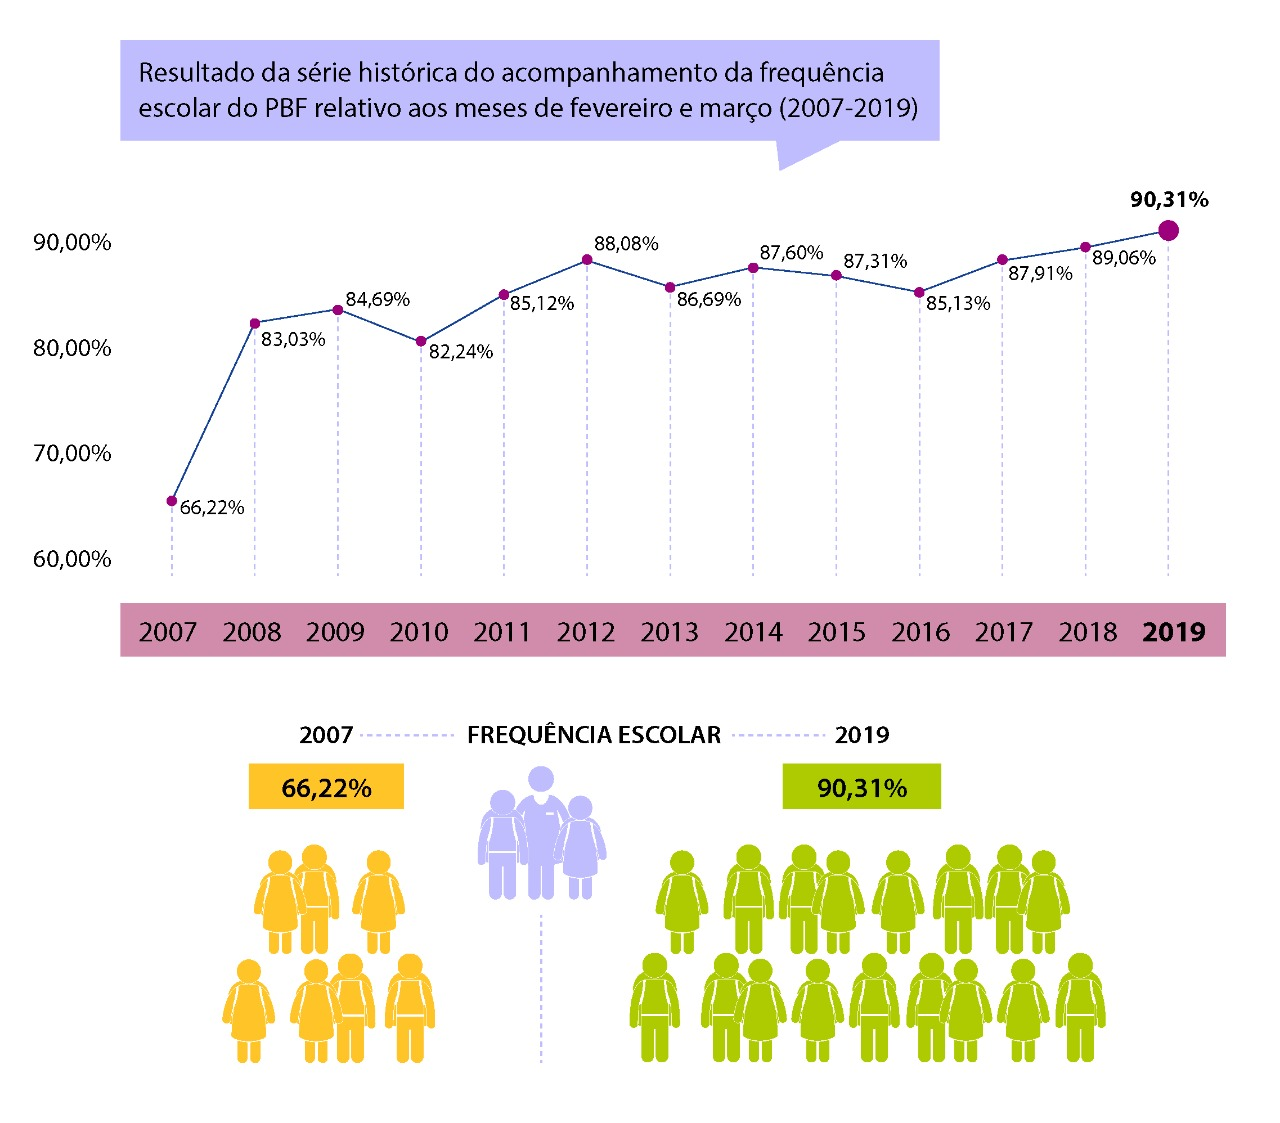
\includegraphics[width=0.46\linewidth]{Textuais/Imagens/image1.png}
    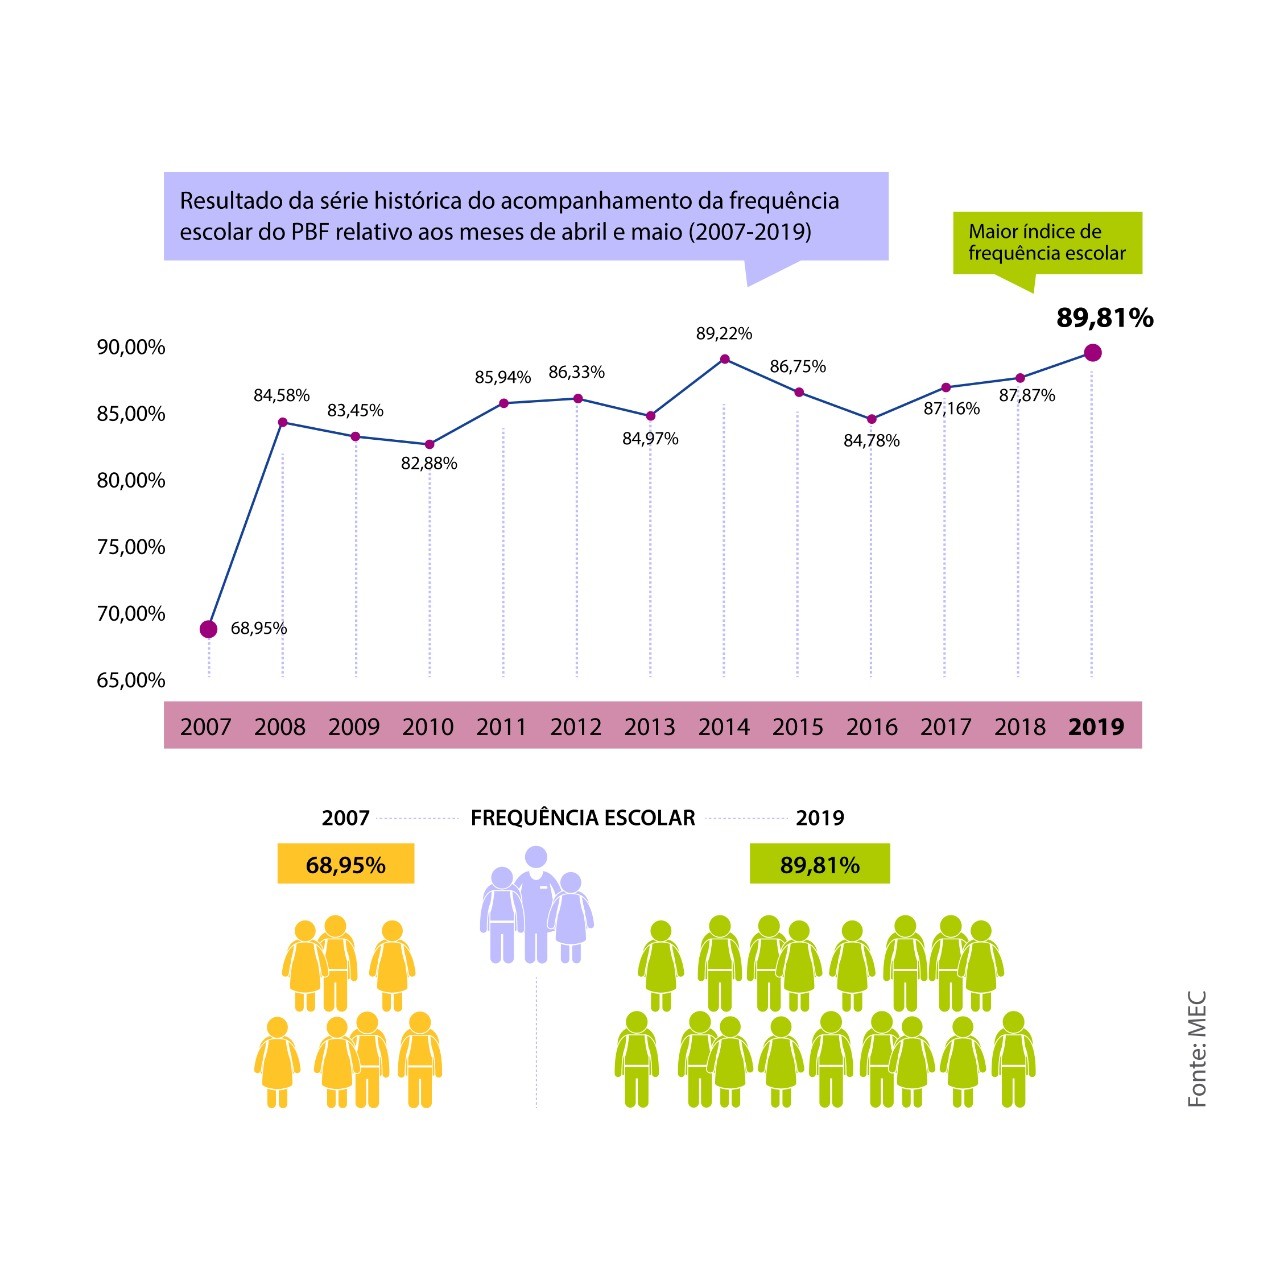
\includegraphics[width=0.46\linewidth]{Textuais/Imagens/image.png}
    \caption{Histórico de frequência de estudantes no Brasil entre os meses de fevereiro a março, e de março a abril de 2019.}
    \label{fig:my_label}
\end{figure}


O Sistema Presença tem limitações importantes. Como o objetivo deste sistema é fornecer dados para o Bolsa Família, apenas alunos beneficiários deste programa têm sua frequência coletada. Além disso, a frequência é coletada com granularidade mensal. Isto impossibilita o desenvolvimento de ferramentas de alerta de evasão, baseadas em Inteligência Artificial, que sejam capazes de detectar padrões nos dados e permitam ações de combate à evasão em um estágio precoce. Por outro lado, não há a integração dos dados de frequência com outros dados relevantes do estudante, como dados de desempenho escolar. Embora o Sistema Presença ainda esteja em fase de implementação, desde o início dos anos 2000 houveram estudos foram conduzidos com o objetivo de resolver o problema de coleta de dados de frequência de forma mais eficiente \cite{Soligo_2010}. É o caso do trabalho de \citeonline{pereira:2012}, que apresenta uma proposta de monitoramento do estudante no momento de chegada e saída da instituição, sendo realizada em tempo real a comunicação aos responsáveis através do envio de SMS. Adicionalmente, será possível a geração de relatórios acerca da frequência escolar do aluno. A utilização da aplicação proposta visa tornar o controle de frequência mais rápido e eficiente, além de proporcionar a comunicação dos dados coletados aos responsáveis do discente, estabelecendo a sensação de segurança por parte da instituição. Além da frequência, há dispositivos que buscam coletar outros tipos de dados de alunos em sala de aula, como demonstrado no projeto de \citeonline{ferreira:2022}. Neste projeto, foram utilizados objetos vestíveis para detectar os movimentos das crianças do ensino fundamental, a fim de observar o comportamento dos alunos em sala de aula e compreender melhor a rotina escolar. A metodologia utilizada para coletar os dados de movimento das crianças foi a utilização de um dispositivo \textit{wearable Actigraph GT9X Link}, que possui dois acelerômetros e um giroscópio, sendo estes os sensores de captação de movimento. As informações geradas tratam-se de registros em arquivo dos pontos dos eixos de (x, y, z) de cada um dos sensores para cada centésimo de segundo. Para ser traçado o perfil dos estudantes voluntários, foram enviados formulários aos responsáveis que envolviam perguntas como idade, peso, altura, sexo, mão com a qual escreve e se o aluno possui alguma deficiência diagnosticada. Durante a coleta de dados, foram feitas anotações específicas de todos os movimentos, atividades e atenção de cada aluno por um período de 30 minutos, e os demais movimentos no restante do tempo foram anotados apenas quando tratavam-se de levantar, sentar, andar e sair da sala. Por mais que o estudo não fosse conclusivo e não apresentasse resultados específicos da coleta de dados de movimento das crianças, foi concluído que a utilização de sensores vestíveis em sala de aula pode auxiliar o professor a melhorar a qualidade das palestras, especialmente se as informações forem fornecidas em tempo real, principalmente quando os sensores conseguem estimar o nível de engajamento dos alunos na aula e fornecem essa informação diretamente ao educador.

Contudo, é importante reforçar que a coleta de dados educacionais no Brasil apresenta desafios que vão além da infraestrutura de tecnologia da informação. Em regiões mais remotas do país, como comunidades ribeirinhas e áreas rurais, muitas escolas têm dificuldades para enviar e receber informações por meio de sistemas eletrônicos \cite{Ribeirinhas:2021}. Além disso, a realidade das escolas que atendem adolescentes em conflito com a lei, como a Fundação Casa (antiga Febem), também apresenta dificuldades para a coleta de dados educacionais: Em primeiro lugar, muitos desses jovens chegam à instituição com histórico de evasão escolar e baixa escolaridade, o que dificulta o acompanhamento de sua trajetória educacional. A rotatividade de professores e funcionários nessas instituições, aliada a uma infraestrutura muitas vezes precária, pode dificultar o registro e a organização dos dados educacionais dos alunos. Por fim, há ainda a questão da própria natureza das atividades desenvolvidas nessas instituições, que podem ser muito diferentes das atividades escolares convencionais e, portanto, requerem uma avaliação mais específica e adaptada. O atendimento educacional dessas instituições muitas vezes é feito de forma precária e com poucos recursos, o que pode prejudicar a coleta de informações precisas sobre a frequência e o desempenho dos estudantes \cite{Morais2019}. Essas diferenças no contexto educacional brasileiro tornam ainda mais desafiadora a tarefa de coletar e analisar dados educacionais para subsidiar políticas públicas efetivas.

Em suma, a pluralidade brasileira apresenta desafios significativos para a coleta e análise de dados educacionais. Embora iniciativas como o Cadastro Único para Programas Sociais e o Sistema Presença tenham sido criadas para padronizar as informações sobre a frequência escolar e a vulnerabilidade social das famílias, ainda existem muitos obstáculos a serem superados. A infraestrutura de tecnologia da informação, por exemplo, é um desafio em regiões remotas, e a rotatividade de professores e funcionários em instituições como a Fundação Casa pode dificultar o registro e a organização dos dados educacionais dos alunos. Portanto, novas pesquisas podem ser realizadas para aprimorar essas iniciativas e desenvolver soluções tecnológicas que possam superar esses desafios e garantir a coleta de informações precisas sobre a educação no Brasil. Também é importante ressaltar que a avaliação das atividades educacionais em instituições específicas, como a Fundação Casa, requer uma abordagem mais específica e adaptada, uma vez que essas atividades podem ser muito diferentes das atividades escolares convencionais.




%%%%%%%%%%%%%%%%%%%%%%%%%%%

\section{Análise Comparativa}


Nesta seção, será realizada uma análise comparativa entre os trabalhos relacionados e os dados coletados para a pesquisa de detecção de padrões em relação à presença dos estudantes no ensino básico brasileiro. Os trabalhos relacionados abordam diferentes aspectos da análise de dados educacionais e fornecem conclusões relevantes para a compreensão dos padrões de frequência dos alunos. Por mais que os trabalhos relacionados no exterior e no Brasil tenham grande enfoque na aplicação e otimização de sistemas de frequência, é importante que sejam estudados para que sejam percebidas quais as variáveis mais relevantes durante a coleta de frequência escolar. Sendo assim, é importante destacar que o trabalho atual não irá focar na aplicação de um novo sistema de frequência, e sim, em aplicar algoritmos de LA e EDM em dados que serão coletados futuramente, o que já se torna a diferença principal entre os trabalhos vistos nas seções \ref{sec:exterior} e \ref{sec:brasil}. Ao comparar esses trabalhos relacionados com a pesquisa proposta, observa-se que todos eles compartilham o objetivo comum de compreender e melhorar a frequência dos alunos no ensino básico. No entanto, cada estudo e país possui suas peculiaridades e desafios específicos, o que demanda abordagens adaptadas às suas realidades.

O estudo realizado por \citeonline{Thesis:2019} aborda a aplicação de técnicas de análise de dados para compreender o comportamento dos alunos em relação à frequência escolar. A autora utiliza técnicas de aprendizado de máquina para analisar os dados de frequência dos alunos e identificar padrões que possam contribuir para melhorar o desempenho acadêmico. A metodologia adotada incluiu a coleta de dados quantitativos sobre a frequência dos alunos e a aplicação de técnicas estatísticas avançadas para análise desses dados. Por outro lado, a dissertação de \citeonline{moissa2016} tem foco na avaliação do impacto das ferramentas de aprendizagem analítica (LA) na interação, desempenho e satisfação dos alunos em ambientes virtuais de aprendizagem. Embora o contexto seja diferente do estudo proposto, existe uma relevância em comum, que é entender como as ferramentas de LA podem ser utilizadas para aprimorar a experiência de aprendizagem dos estudantes. A autora conduziu um experimento com usuários reais, coletando dados sobre a interação dos alunos com a ferramenta e utilizando técnicas estatísticas e de Mineração de Dados para análise dos dados coletados. A abordagem mista, que combinou métodos quantitativos e qualitativos, proporcionou uma compreensão mais abrangente dos resultados obtidos. No entanto, o presente trabalho tem um foco distinto, concentrando-se em outras áreas, como a aplicação da detecção de padrões e a visualização das informações dos resultados obtidos. Busca-se explorar como essas técnicas podem ser utilizadas para identificar padrões de frequência escolar e visualizar esses dados de forma compreensível e significativa. Dessa forma, pretende-se oferecer insights valiosos aos educadores e formuladores de políticas educacionais, permitindo uma tomada de decisão embasada na compreensão dos padrões de frequência dos alunos. Assim, apesar das semelhanças entre os estudos mencionados, o atual trabalho busca aprimorar o conhecimento na área, concentrando-se em aspectos específicos da análise de dados e visualização das informações sobre a frequência escolar, com o objetivo de contribuir para a melhoria da experiência educacional dos alunos.

Na seção \ref{sec:exterior}, foram apresentadas iniciativas no exterior que abordam a detecção de frequência escolar por meio de tecnologias avançadas, como detecção facial, RFID e dispositivos vestíveis. Essas abordagens demonstram a diversidade de soluções utilizadas para coletar e analisar dados de frequência dos alunos. Os estudos apresentados destacam a precisão e eficiência das tecnologias utilizadas, além de considerar aspectos como segurança, portabilidade e disponibilidade dos dados. Já na seção \ref{sec:brasil}, foram abordadas iniciativas no Brasil, como o Cadastro Único para Programas Sociais (CadUnico) e o Sistema Presença. O CadUnico é uma fonte de dados importante para monitorar a escolaridade no país, registrando informações sobre a frequência dos alunos. O Sistema Presença, por sua vez, busca padronizar as informações sobre a frequência escolar em todo o país. Ele é utilizado pelos gestores educacionais para registrar a presença dos alunos nas escolas, permitindo o monitoramento em tempo real da frequência e a identificação de possíveis problemas de evasão escolar. O sistema também auxilia na tomada de decisões e na formulação de políticas públicas para garantir a universalização do acesso à educação, e o \textit{software} é o que servirá para aplicação do NEES.
\chapter{Contexto da pesquisa}

% \textcolor{red}{contexto dos projetos, desde o início, inserção dos projetos, o projeto que estou inserida (frequência), foi feita a análise da arquitetura, mas não teve a etapa da coleta. nesse caso, foi dado u passo atrás, entrou em contato com outro grupo do nees, do sistema alerta preventivo, dados não são públicos, não serão divulgados, mas o instrumento e estrutura estão nesse anexo}



No estágio inicial deste trabalho de conclusão de curso, a abordagem consistia na análise da arquitetura do sistema, fornecida pelo NEES, juntamente com uma revisão da literatura nacional e internacional sobre sistemas de coleta de frequência e algoritmos de reconhecimento de padrões baseados em machine learning. A expectativa era que os dados adquiridos pudessem ser prontamente aplicados à arquitetura futura do Sistema Presença do TED 11476. No entanto, devido à indisponibilidade dos dados desse TED específico, foi necessário um redirecionamento metodológico. Em contato com o TED 10974, responsável pelo Sistema Alerta Preventivo (SAP), foi possível obter acesso a dados não públicos do SAP. Esses dados, embora não sejam divulgados publicamente, foram fundamentais para a análise proposta, utilizando o instrumento e a estrutura fornecidos no Anexo 1, em substituição aos dados originais não obtidos.

A pesquisa teve início com a intenção de identificar padrões na base de dados proveniente do sistema de frequência do TED 11476, a qual almeja reformular o atual Sistema Presença, responsável por coletar a frequência escolar de estudantes do ensino básico vinculados ao programa Bolsa Família no Brasil \cite{BolsaFamilia}. Foi apresentada a futura arquitetura da base de dados do sistema, bem como o modelo entidade-relacionamento da coleta de frequência e como os professores teriam suas respectivas conexões. Contudo, pelo teste piloto marcado para acontecer em setembro não ter coletado dados de frequência de estudantes, e por não ter sido possível conseguir uma base de dados legada do Sistema Presença vigente, a etapa do estudo de dados do TED 11476 não pôde ser concretizada conforme inicialmente previsto. Na tentativa de se realizar uma base de dados sintética, foi solicitada a base do TED 10974, esperando compreender diferentes motivações de evasão escolar a serem replicadas na arquitetura disponibilizada. Porém, embora tenha implicado em uma regressão no processo planejado, foi optado pelo foco nos dados disponibilizados pelo TED 10974, utilizando os algoritmos estudados anteriormente para aplicação nessa base.

Assim, o foco metodológico da pesquisa passou a envolver a análise da arquitetura do SAP, utilizando os dados disponíveis. Este passo foi considerado necessário para avançar no entendimento dos fatores de risco de evasão escolar. Este ajuste metodológico permitiu uma continuidade efetiva na análise do contexto do Sistema Alerta Preventivo, oferecendo insights valiosos para a compreensão dos fatores relacionados à evasão escolar no contexto específico do projeto.

Tanto o questionário das perguntas relacionadas a evasão quanto as perguntas sociodemográficas estão disponibilizadas neste trabalho como Anexo 1.


\section{Questionário Sistema Alerta Preventivo}
\label{cap:analises-sap}

% Os dados disponibilizados foram organizados de acordo com os relacionamentos dos estudantes com diversos fatores chamados de dimensão de risco estudante-escola (E-ESC), Estudante - profissionais da escola (e-prof), Estudante-familia(e-fam), estudante-comunidade (E-COM) e também com seus semelhantes estudante-estudante (e-est).
% Dos 17 mil respondentes das 35 perguntas e dentro de cada tipo de relacionamento organizou-se os fatores de risco dentro de cada relacionamento com tres perguntas em cada um. Condições Materiais da Escola (e-esc1), condicões Materias do(a) estudante (E-ESC2),  Inflexibilidade
% Pedagógica
% (E-PROF1), Qualidade
% Pedagógica
% (E-PROF2), Suporte Familiar
% (E-FAM1), Gravidez/parentalidade/
% atividades de cuidado
% (E-FAM2), Medidas
% socioeducativas e
% contextos de
% violência(E-COM1), Acessibilidade e
% frequência escolar
% (E-COM2), Distanciamento
% escola –
% comunidade
% (E-COM3), Significados da
% Escolarização/
% Engajamento
% (E-EST1), Aspectos
% Emocionais e
% Afetivos(E-EST2), Reprovações e
% distorção idade –
% série. (E-EST3).

O banco de dados disponibilizado pelo NEES, referente ao SAP, foi realizado com 17.110 estudantes de forma presencial em dezembro de 2022. O banco compilou e categorizou dados cruciais para compreender as multifacetadas dimensões de risco de evasão, que podem ser afetados a partir da relação entre estudantes e seus ambientes escolares, domésticos e comunitários, bem como suas interações entre pares. Este arcabouço de informação, constituído por respostas de alunos do primeiro ao nono ano do ensino fundamental de 308 escolas diferentes, a 36 questões distintas, constitui uma base sólida para a investigação das causas subjacentes à evasão escolar. Cada pergunta era respondida por meio de uma escala de Likert, onde as respostas eram valores inteiros entre 1 (Discordo Totalmente) e 7 (Concordo Totalmente), sendo que os estudantes podiam optar por não responder às perguntas, atribuindo valor 0 à pergunta. As perguntas foram separadas em grupos de análise de fatores de risco, e dois ou três fatores eram agrupados em uma única dimensão analisada. Esta organização é apresentada na Tabela \ref{tab:questionario}.

Dentro deste contexto, a dimensão \textbf{Estudante-Escola (E-ESC)} lança luz sobre as condições materiais das instituições de ensino. Este aspecto envolve não apenas a infraestrutura física mas também recursos didáticos essenciais para um ambiente de aprendizagem eficaz. Além disso, examina-se a realidade material dos próprios estudantes, percebendo como a escassez de recursos pode influenciar negativamente a permanência na escola.

Por outro lado, a relação \textbf{Estudante-Profissionais da Escola (E-PROF)} aborda a rigidez e a qualidade pedagógica. Aqui, a inflexibilidade pedagógica surge como um fator de risco potencial, pois pode desencorajar os estudantes cujas necessidades educacionais variam. Em contrapartida, a qualidade do ensino detém uma influência crítica, já que a excelência pedagógica e a atenção individualizada podem diminuir as chances de abandono escolar.

No que tange à dimensão \textbf{Estudante-Família (E-FAM)}, o suporte familiar é analisado como um alicerce essencial para a continuidade educacional. Desafios como gravidez na adolescência, parentalidade precoce e obrigações de cuidado podem desviar a atenção e os recursos dos estudantes da educação para responsabilidades familiares, aumentando o risco de evasão.

A relação \textbf{Estudante-Comunidade (E-COM)} explora como medidas socioeducativas e a prevalência de violência no entorno podem criar barreiras ao acesso e à frequência escolar, além de como a desconexão entre a escola e a comunidade pode acentuar a sensação de isolamento dos estudantes, diminuindo a valorização da educação em seus contextos de vida.

Finalmente, na esfera \textbf{Estudante-Estudante (E-EST)}, observa-se o impacto do engajamento escolar e os significados atribuídos à escolarização, bem como as interações emocionais e afetivas entre os estudantes, e como repetências e defasagens idade-série podem desmotivar os alunos e conduzi-los ao abandono do sistema educacional.

    
\begin{longtable}{|@{}>{\centering\arraybackslash}p{0.25\textwidth}| >{\centering\arraybackslash\scriptsize}p{\dimexpr 0.23\textwidth - 24pt\relax}| >{\centering\arraybackslash}p{0.12\textwidth}| >{\raggedright\arraybackslash\scriptsize}p{0.35\textwidth}@{}|}
\caption{Perguntas do questionário associadas a fatores e dimensões}
\label{tab:questionario}

\hline
\textbf{Dimensão de Risco} &
  \textbf{Fatores de Risco} &
  \textbf{\begin{tabular}[c]{@{}c@{}}Código da\\ Pergunta\end{tabular}} &
  \multicolumn{1}{c|}{\textbf{Itens}} \\ \hline
\endhead
\multirow{6}{*}{\textbf{\begin{tabular}[c]{@{}c@{}}Estudante –\\ Escola (E-ESC)\end{tabular}}} &
  \multirow{3}{*}{\begin{tabular}[c]{@{}c@{}}Condições\\ Materiais da Escola\\ (E-ESC1)\end{tabular}} &
  Q3 &
  \begin{tabular}[c]{@{}l@{}}A alimentação oferecida na escola me faz\\ pensar em não ir para ela.\end{tabular} \\ \cline{3-4} 
 &
   &
  Q4 &
  \begin{tabular}[c]{@{}l@{}}Pensei em me afastar da escola por não ter\\ equipamentos adequados para lidar com as\\ condições do clima (ventilador, aquecedor,\\ ar condicionado).\end{tabular} \\ \cline{3-4} 
 &
   &
  Q23 &
  \begin{tabular}[c]{@{}l@{}}Não poder usar a internet na escola é algo\\ que me faz querer me afastar.\end{tabular} \\ \cline{2-4} 
 &
  \multirow{3}{*}{\begin{tabular}[c]{@{}c@{}}Condições\\ Materiais do(a)\\ Estudante (E-ESC2)\end{tabular}} &
  Q9 &
  \begin{tabular}[c]{@{}l@{}}Pensei em sair da escola porque não tenho\\ um bom espaço em casa para me\\ concentrar nos estudos.\end{tabular} \\ \cline{3-4} 
 &
   &
  Q28 &
  \begin{tabular}[c]{@{}l@{}}Possuo o material escolar adequado para\\ acompanhar as aulas (lápis, caderno, etc.).\end{tabular} \\ \cline{3-4} 
 &
   &
  Q36 &
  \begin{tabular}[c]{@{}l@{}}Não possuo o fardamento escolar\\ adequado.\end{tabular} \\ \hline
\multirow{6}{*}{\textbf{\begin{tabular}[c]{@{}c@{}}Estudante –\\ Profissionais da\\ Escola (E-PROF)\end{tabular}}} &
  \multirow{3}{*}{\begin{tabular}[c]{@{}c@{}}Inflexibilidade\\ Pedagógica\\ (E-PROF1)\end{tabular}} &
  Q13 &
  \begin{tabular}[c]{@{}l@{}}Pensei em me afastar da escola pela\\ quantidade de regras que ela tem.\end{tabular} \\ \cline{3-4} 
 &
   &
  Q18 &
  \begin{tabular}[c]{@{}l@{}}Penso em deixar a escola porque ela não\\ me permite fazer atividades como música,\\ dança, teatro, desenho.\end{tabular} \\ \cline{3-4} 
 &
   &
  Q22 &
  \begin{tabular}[c]{@{}l@{}}Pensei em abandonar a escola por não\\ poder praticar os esportes que eu queria.\end{tabular} \\ \cline{2-4} 
 &
  \multirow{3}{*}{\begin{tabular}[c]{@{}c@{}}Qualidade\\ Pedagógica\\ (E-PROF2)\end{tabular}} &
  Q12 &
  \begin{tabular}[c]{@{}l@{}}Pensei em abandonar a escola pois os (as)\\ professores (as) faltam muito.\end{tabular} \\ \cline{3-4} 
 &
   &
  Q19 &
  \begin{tabular}[c]{@{}l@{}}Pensei em abandonar a escola porque as\\ salas têm mais estudantes do que os\\ professores conseguem dar atenção.\end{tabular} \\ \cline{3-4} 
 &
   &
  Q20 &
  \begin{tabular}[c]{@{}l@{}}Pensei em abandonar a escola pois as aulas\\ são repetitivas e cansativas.\end{tabular} \\ \hline
\multirow{6}{*}{\textbf{\begin{tabular}[c]{@{}c@{}}Estudante –\\ Família (E-FAM)\end{tabular}}} &
  \multirow{3}{*}{\begin{tabular}[c]{@{}c@{}}Suporte Familiar\\ (E-FAM1)\end{tabular}} &
  \multicolumn{1}{c|}{Q16} &
  \begin{tabular}[c]{@{}l@{}}Alguém da minha família já sugeriu que eu\\ deixasse a escola.\end{tabular} \\ \cline{3-4} 
 &
   &
  \multicolumn{1}{c|}{Q30} &
  \begin{tabular}[c]{@{}l@{}}Meus pais/responsáveis não podem vir à\\ escola quando são chamados.\end{tabular} \\ \cline{3-4} 
 &
   &
  \multicolumn{1}{c|}{Q32} &
  \begin{tabular}[c]{@{}l@{}}Minha mãe, ou a pessoa que cuida de mim,\\ não terminou a escola.\end{tabular} \\ \cline{2-4} 
 &
  \multirow{3}{*}{\begin{tabular}[c]{@{}c@{}}Gravidez/parentalidade/\\ atividades de cuidado\\ (E-FAM2)\end{tabular}} &
  \multicolumn{1}{c|}{Q15} &
  \begin{tabular}[c]{@{}l@{}}Já faltei à escola ou deixei de fazer lição\\ de casa por ter que ajudar em atividades\\ de casa (cozinhar, limpar, cuidar de\\ irmãos etc).\end{tabular} \\ \cline{3-4} 
 &
   &
  \multicolumn{1}{c|}{Q21} &
  \begin{tabular}[c]{@{}l@{}}Já pensei em abandonar a escola por ter\\ tido e/ou ter um problema de saúde na\\ família.\end{tabular} \\ \cline{3-4} 
 &
   &
  \multicolumn{1}{c|}{Q31} &
  \begin{tabular}[c]{@{}l@{}}Já aconteceu de eu não poder continuar na\\ escola por causa de uma gravidez, seja\\ minha ou da minha parceira.\end{tabular} \\ \hline

  \multirow{9}{*}{\textbf{\begin{tabular}[c]{@{}c@{}}Estudante –\\ Comunidade\\ (E-COM)\end{tabular}}} &
  \multirow{3}{*}{\begin{tabular}[c]{@{}c@{}}Medidas\\ socioeducativas e\\ contextos de\\ violência(E-COM1)\end{tabular}} &
  Q29 &
  \begin{tabular}[c]{@{}l@{}}Meus colegas frequentemente abusam de\\ álcool ou drogas.\end{tabular} \\ \cline{3-4} 
 &
   &
  Q33 &
  \begin{tabular}[c]{@{}l@{}}Já tive/tenho contato com o Conselho\\ Tutelar.\end{tabular} \\ \cline{3-4} 
 &
   &
  Q34 &
  \begin{tabular}[c]{@{}l@{}}É comum que na minha escola estudantes\\ enfrentem problemas com a justiça.\end{tabular} \\ \cline{2-4} 
 &
  \multirow{3}{*}{\begin{tabular}[c]{@{}c@{}}Acessibilidade e\\ frequência escolar\\ (E-COM2)\end{tabular}} &
  Q8 &
  \begin{tabular}[c]{@{}l@{}}Já pensei em deixar a escola porque não\\ tenho aulas sobre a história ou questões\\ importantes da minha comunidade ou\\ cidade.\end{tabular} \\ \cline{3-4} 
 &
   &
  Q11 &
  \begin{tabular}[c]{@{}l@{}}Já pensei em deixar a escola porque ela\\ não respeita a religião que eu pratico.\end{tabular} \\ \cline{3-4} 
 &
   &
  Q14 &
  \begin{tabular}[c]{@{}l@{}}Já pensei em deixar a escola porque com\\ frequência ela é alvo de violência\\ (vandalismo, assaltos, pichações, toque de\\ recolher e etc).\end{tabular} \\ \cline{2-4} 
 &
  \multirow{3}{*}{\begin{tabular}[c]{@{}c@{}}Distanciamento\\ escola –\\ comunidade\\ (E-COM3)\end{tabular}} &
  Q7 &
  \begin{tabular}[c]{@{}l@{}}Já considerei abandonar a escola por ter\\ tido e/ou ter um problema de saúde.\end{tabular} \\ \cline{3-4} 
 &
   &
  Q17 &
  \begin{tabular}[c]{@{}l@{}}Pensei em abandonar a escola porque não\\ tenho dinheiro suficiente para vir ou\\ porque o caminho até aqui é muito difícil.\end{tabular} \\ \cline{3-4} 
 &
   &
  Q25 &
  Falto às aulas mais do que é permitido. \\ \hline
  
\multirow{9}{*}{\textbf{\begin{tabular}[c]{@{}c@{}}Estudante –\\ Estudante\\ (E-EST)\end{tabular}}} &
  \multicolumn{1}{l|}{\multirow{3}{*}{\begin{tabular}[c]{@{}l@{}}Significados da\\ Escolarização/\\ Engajamento\\ (E-EST1)\end{tabular}}} &
  Q5 &
  \begin{tabular}[c]{@{}l@{}}Já pensei em abandonar a escola porque\\ não vejo como ela vai me ajudar a mudar\\ minha vida para melhor.\end{tabular} \\ \cline{3-4} 
 &
  \multicolumn{1}{l|}{} &
  Q6 &
  \begin{tabular}[c]{@{}l@{}}Pensei em deixar a escola pois ela não\\ trata dos assuntos atuais.\end{tabular} \\ \cline{3-4} 
 &
  \multicolumn{1}{l|}{} &
  Q10 &
  \begin{tabular}[c]{@{}l@{}}Já pensei em abandonar a escola pois ela\\ não me prepara para os empregos que\\ quero ter no futuro.\end{tabular} \\ \cline{2-4} 
 &
 
  \multicolumn{1}{l|}{\multirow{3}{*}{\begin{tabular}[c]{@{}l@{}}Aspectos\\ Emocionais e\\ Afetivos(E-EST2)\end{tabular}}} &
  Q1 &
  \begin{tabular}[c]{@{}l@{}}Às vezes, me sinto triste ou deprimido(a),\\ e isso me faz pensar em deixar a escola.\end{tabular} \\ \cline{3-4} 
 &
  \multicolumn{1}{l|}{} &
  Q2 &
  \begin{tabular}[c]{@{}l@{}}Sinto que sou incapaz de concluir meus\\ estudos e por isso penso em abandonar a\\ escola.\end{tabular} \\ \cline{3-4} 
 &
  \multicolumn{1}{l|}{} &
  Q24 &
  \begin{tabular}[c]{@{}l@{}}Já pensei em deixar a escola porque\\ meus/minhas colegas não me tratam bem.\end{tabular} \\ \cline{2-4} 
 &
  \multicolumn{1}{l|}{\multirow{3}{*}{\begin{tabular}[c]{@{}l@{}}Reprovações e\\ distorção idade –\\ série. (E-EST3)\end{tabular}}} &
  Q26 &
  \begin{tabular}[c]{@{}l@{}}Acredito que tenho mais dificuldade de\\ acompanhar as aulas do que os outros\\ colegas.\end{tabular} \\ \cline{3-4} 
 &
  \multicolumn{1}{l|}{} &
  Q27 &
  \begin{tabular}[c]{@{}l@{}}Minhas notas em Poutuguês e/ou\\ Matemática estão abaixo da média.\end{tabular} \\ \cline{3-4} 
 &
  \multicolumn{1}{l|}{} &
  Q35 &
  \begin{tabular}[c]{@{}l@{}}Não estou na série que deveria estar para\\ a minha idade.\end{tabular} \\ \hline
\end{longtable}
\fonte{NEES - TED 10479 (2022)}

% \begin{table}[ht]
% \centering
% \resizebox{\textwidth}{!}{%
% \begin{tabular}{|c|c|c|l|}
% \hline
% \textbf{Dimensão de Risco} &
%   \textbf{Fatores de Risco} &
%   \textbf{\begin{tabular}[c]{@{}c@{}}Código da\\ Pergunta\end{tabular}} &
%   \multicolumn{1}{c|}{\textbf{Itens}} \\ \hline
% \multirow{6}{*}{\textbf{\begin{tabular}[c]{@{}c@{}}Estudante –\\ Escola (E-ESC)\end{tabular}}} &
%   \multirow{3}{*}{\begin{tabular}[c]{@{}c@{}}Condições\\ Materiais da Escola\\ (E-ESC1)\end{tabular}} &
%   Q3 &
%   \begin{tabular}[c]{@{}l@{}}A alimentação oferecida na escola me faz\\ pensar em não ir para ela.\end{tabular} \\ \cline{3-4} 
%  &
%    &
%   Q4 &
%   \begin{tabular}[c]{@{}l@{}}Pensei em me afastar da escola por não ter\\ equipamentos adequados para lidar com as\\ condições do clima (ventilador, aquecedor,\\ ar condicionado).\end{tabular} \\ \cline{3-4} 
%  &
%    &
%   Q23 &
%   \begin{tabular}[c]{@{}l@{}}Não poder usar internet na escola é algo\\ que me faz querer me afastar.\end{tabular} \\ \cline{2-4} 
%  &
%   \multirow{3}{*}{\begin{tabular}[c]{@{}c@{}}Condições\\ Materiais do(a)\\ Estudante (E-ESC2)\end{tabular}} &
%   Q9 &
%   \begin{tabular}[c]{@{}l@{}}Pensei em sair da escola porque não tenho\\ um bom espaço em casa para me\\ concentrar nos estudos.\end{tabular} \\ \cline{3-4} 
%  &
%    &
%   Q28 &
%   \begin{tabular}[c]{@{}l@{}}Possuo o material escolar adequado para\\ acompanhar as aulas (lápis, caderno, etc.).\end{tabular} \\ \cline{3-4} 
%  &
%    &
%   Q36 &
%   \begin{tabular}[c]{@{}l@{}}Não possuo o fardamento escolar\\ adequado.\end{tabular} \\ \hline
% \multirow{6}{*}{\textbf{\begin{tabular}[c]{@{}c@{}}Estudante –\\ Profissionais da\\ Escola (E-PROF)\end{tabular}}} &
%   \multirow{3}{*}{\begin{tabular}[c]{@{}c@{}}Inflexibilidade\\ Pedagógica\\ (E-PROF1)\end{tabular}} &
%   Q13 &
%   \begin{tabular}[c]{@{}l@{}}Pensei em me afastar da escola pela\\ quantidade de regras que ela tem.\end{tabular} \\ \cline{3-4} 
%  &
%    &
%   Q18 &
%   \begin{tabular}[c]{@{}l@{}}Penso em deixar a escola porque ela não\\ me permite fazer atividades como música,\\ dança, teatro, desenho.\end{tabular} \\ \cline{3-4} 
%  &
%    &
%   Q22 &
%   \begin{tabular}[c]{@{}l@{}}Pensei em abandonar a escola por não\\ poder praticar os esportes que eu queria.\end{tabular} \\ \cline{2-4} 
%  &
%   \multirow{3}{*}{\begin{tabular}[c]{@{}c@{}}Qualidade\\ Pedagógica\\ (E-PROF2)\end{tabular}} &
%   Q12 &
%   \begin{tabular}[c]{@{}l@{}}Pensei em abandonar a escola pois os (as)\\ professores (as) faltam muito.\end{tabular} \\ \cline{3-4} 
%  &
%    &
%   Q19 &
%   \begin{tabular}[c]{@{}l@{}}Pensei em abandonar a escola porque as\\ salas têm mais estudantes do que os\\ professores conseguem dar atenção.\end{tabular} \\ \cline{3-4} 
%  &
%    &
%   Q20 &
%   \begin{tabular}[c]{@{}l@{}}Pensei em abandonar a escola pois as aulas\\ são repetitivas e cansativas.\end{tabular} \\ \hline
% \multirow{6}{*}{\textbf{\begin{tabular}[c]{@{}c@{}}Estudante –\\ Família (E-FAM)\end{tabular}}} &
%   \multirow{3}{*}{\begin{tabular}[c]{@{}c@{}}Suporte Familiar\\ (E-FAM1)\end{tabular}} &
%   \multicolumn{1}{c|}{Q16} &
%   \begin{tabular}[c]{@{}l@{}}Alguém da minha família já sugeriu que eu\\ deixasse a escola.\end{tabular} \\ \cline{3-4} 
%  &
%    &
%   \multicolumn{1}{c|}{Q30} &
%   \begin{tabular}[c]{@{}l@{}}Meus pais/responsáveis não podem vir à\\ escola quando são chamados.\end{tabular} \\ \cline{3-4} 
%  &
%    &
%   \multicolumn{1}{c|}{Q32} &
%   \begin{tabular}[c]{@{}l@{}}Minha mãe, ou a pessoa que cuida de mim,\\ não terminou a escola.\end{tabular} \\ \cline{2-4} 
%  &
%   \multirow{3}{*}{\begin{tabular}[c]{@{}c@{}}Gravidez/parentalidade/\\ atividades de cuidado\\ (E-FAM2)\end{tabular}} &
%   \multicolumn{1}{c|}{Q15} &
%   \begin{tabular}[c]{@{}l@{}}Já faltei à escola ou deixei de fazer lição\\ de casa por ter que ajudar em atividades\\ de casa (cozinhar, limpar, cuidar de\\ irmãos etc).\end{tabular} \\ \cline{3-4} 
%  &
%    &
%   \multicolumn{1}{c|}{Q21} &
%   \begin{tabular}[c]{@{}l@{}}Já pensei em abandonar a escola por ter\\ tido e/ou ter um problema de saúde na\\ família.\end{tabular} \\ \cline{3-4} 
%  &
%    &
%   \multicolumn{1}{c|}{Q31} &
%   \begin{tabular}[c]{@{}l@{}}Já aconteceu de eu não poder continuar na\\ escola por causa de uma gravidez, seja\\ minha ou da minha parceira.\end{tabular} \\ \hline
% \end{tabular}%
% }
% \caption{Perguntas do questionário associadas a fatores e dimensões}
% \end{table}


% \begin{table}[ht]
% \centering
% \resizebox{\textwidth}{!}{%
% \begin{tabular}{|c|c|c|l|}
% \hline
% \textbf{Dimensão de Risco} &
%   \textbf{Fatores de Risco} &
%   \multicolumn{1}{c|}{\textbf{\begin{tabular}[c]{@{}c@{}}Código da\\ Pergunta\end{tabular}}} &
%   \multicolumn{1}{c|}{\textbf{Itens}} \\ \hline
% \multirow{9}{*}{\textbf{\begin{tabular}[c]{@{}c@{}}Estudante –\\ Comunidade\\ (E-COM)\end{tabular}}} &
%   \multirow{3}{*}{\begin{tabular}[c]{@{}c@{}}Medidas\\ socioeducativas e\\ contextos de\\ violência(E-COM1)\end{tabular}} &
%   Q29 &
%   \begin{tabular}[c]{@{}l@{}}Meus colegas frequentemente abusam de\\ álcool ou drogas.\end{tabular} \\ \cline{3-4} 
%  &
%    &
%   Q33 &
%   \begin{tabular}[c]{@{}l@{}}Já tive/tenho contato com o Conselho\\ Tutelar.\end{tabular} \\ \cline{3-4} 
%  &
%    &
%   Q34 &
%   \begin{tabular}[c]{@{}l@{}}É comum que na minha escola estudantes\\ enfrentem problemas com a justiça.\end{tabular} \\ \cline{2-4} 
%  &
%   \multirow{3}{*}{\begin{tabular}[c]{@{}c@{}}Acessibilidade e\\ frequência escolar\\ (E-COM2)\end{tabular}} &
%   Q8 &
%   \begin{tabular}[c]{@{}l@{}}Já pensei em deixar a escola porque não\\ tenho aulas sobre a história ou questões\\ importantes da minha comunidade ou\\ cidade.\end{tabular} \\ \cline{3-4} 
%  &
%    &
%   Q11 &
%   \begin{tabular}[c]{@{}l@{}}Já pensei em deixar a escola porque ela\\ não respeita a religião que eu pratico.\end{tabular} \\ \cline{3-4} 
%  &
%    &
%   Q14 &
%   \begin{tabular}[c]{@{}l@{}}Já pensei em deixar a escola porque com\\ frequência ela é alvo de violência\\ (vandalismo, assaltos, pichações, toque de\\ recolher e etc).\end{tabular} \\ \cline{2-4} 
%  &
%   \multirow{3}{*}{\begin{tabular}[c]{@{}c@{}}Distanciamento\\ escola –\\ comunidade\\ (E-COM3)\end{tabular}} &
%   Q7 &
%   \begin{tabular}[c]{@{}l@{}}Já considerei abandonar a escola por ter\\ tido e/ou ter um problema de saúde.\end{tabular} \\ \cline{3-4} 
%  &
%    &
%   Q17 &
%   \begin{tabular}[c]{@{}l@{}}Pensei em abandonar a escola porque não\\ tenho dinheiro suficiente para vir ou\\ porque o caminho até aqui é muito difícil.\end{tabular} \\ \cline{3-4} 
%  &
%    &
%   Q25 &
%   Falto às aulas mais do que é permitido. \\ \hline
% \multirow{9}{*}{\textbf{\begin{tabular}[c]{@{}c@{}}Estudante –\\ Estudante\\ (E-EST)\end{tabular}}} &
%   \multicolumn{1}{l|}{\multirow{3}{*}{\begin{tabular}[c]{@{}l@{}}Significados da\\ Escolarização/\\ Engajamento\\ (E-EST1)\end{tabular}}} &
%   Q5 &
%   \begin{tabular}[c]{@{}l@{}}Já pensei em abandonar a escola porque\\ não vejo como ela vai me ajudar a mudar\\ minha vida para melhor.\end{tabular} \\ \cline{3-4} 
%  &
%   \multicolumn{1}{l|}{} &
%   Q6 &
%   \begin{tabular}[c]{@{}l@{}}Pensei em deixar a escola pois ela não\\ trata dos assuntos atuais.\end{tabular} \\ \cline{3-4} 
%  &
%   \multicolumn{1}{l|}{} &
%   Q10 &
%   \begin{tabular}[c]{@{}l@{}}Já pensei em abandonar a escola pois ela\\ não me prepara para os empregos que\\ quero ter no futuro.\end{tabular} \\ \cline{2-4} 
%  &
%   \multicolumn{1}{l|}{\multirow{3}{*}{\begin{tabular}[c]{@{}l@{}}Aspectos\\ Emocionais e\\ Afetivos(E-EST2)\end{tabular}}} &
%   Q1 &
%   \begin{tabular}[c]{@{}l@{}}Às vezes, me sinto triste ou deprimido(a),\\ e isso me faz pensar em deixar a escola.\end{tabular} \\ \cline{3-4} 
%  &
%   \multicolumn{1}{l|}{} &
%   Q2 &
%   \begin{tabular}[c]{@{}l@{}}Sinto que sou incapaz de concluir meus\\ estudos e por isso penso em abandonar a\\ escola.\end{tabular} \\ \cline{3-4} 
%  &
%   \multicolumn{1}{l|}{} &
%   Q24 &
%   \begin{tabular}[c]{@{}l@{}}Já pensei em deixar a escola porque\\ meus/minhas colegas não me tratam bem.\end{tabular} \\ \cline{2-4} 
%  &
%   \multicolumn{1}{l|}{\multirow{3}{*}{\begin{tabular}[c]{@{}l@{}}Reprovações e\\ distorção idade –\\ série. (E-EST3)\end{tabular}}} &
%   Q26 &
%   \begin{tabular}[c]{@{}l@{}}Acredito que tenho mais dificuldade de\\ acompanhar as aulas do que os outros\\ colegas.\end{tabular} \\ \cline{3-4} 
%  &
%   \multicolumn{1}{l|}{} &
%   Q27 &
%   \begin{tabular}[c]{@{}l@{}}Minhas notas em Poutuguês e/ou\\ Matemática estão abaixo da média.\end{tabular} \\ \cline{3-4} 
%  &
%   \multicolumn{1}{l|}{} &
%   Q35 &
%   \begin{tabular}[c]{@{}l@{}}Não estou na série que deveria estar para\\ a minha idade.\end{tabular} \\ \hline
% \end{tabular}%
% }
% \caption{Perguntas do questionário associadas a fatores e dimensões}
% \end{table}


%%%%%%%%%%%%%%%%%%%%%%%%%%%%%%%%%%%%%%
%%%%%%%%%%%%%%%%%%%%%%%%%%%%%%%%%%%%%%
%%%%%%%%%%%%%%%%%%%%%%%%%%%%%%%%%%%%%%
%%%%%%%%%%%%%%%%%%%%%%%%%%%%%%%%%%%%%%

\section{Análises descritivas}



Em uma visão mais ampla, observando-se a Dimensão dos Riscos, os dados permitem uma visão detalhada das percepções e experiências dos estudantes em relação a tais fatores e suas potencialidades dentro de suas escolas e comunidades, bem como em relação à sua saúde emocional e engajamento acadêmico.

A análise das respostas dos estudantes revela informações interessantes sobre a percepção que têm de sua experiência educacional, como pode ser observado na Tabela \ref{tab:estatisticas}. A dimensão ``Estus pfedante – Comunidade (E-COM)'' que inclui aspectos como o impacto da violência e problemas com a justiça, bem como questões de acessibilidade e identificação com o currículo escolar. As médias para estas dimensões (E-COMV) mostram uma pontuação de 1.677947, sugerindo uma percepção relativamente baixa dos riscos associados. Ainda assim, há uma variação considerável, como indicado pelo desvio padrão de 0.873904, que aponta para experiências distintas entre os alunos nesta dimensão.

As preocupações sobre o distanciamento entre a escola e a comunidade, assim como as dificuldades financeiras e de saúde que impactam a frequência às aulas, são também indicativas de barreiras significativas que podem influenciar a decisão dos estudantes de permanecer na escola. Questões de saúde e financeiras, especificamente, parecem ser menos mencionadas como razões para pensar em abandonar a escola, o que é ilustrado pela mediana de 1.333333, indicando que mais da metade dos estudantes classificou estas preocupações abaixo da média de risco percebido.

Quando observa-se a dimensão ``Estudante – Estudante (E-EST)'', é possível observar que os alunos têm uma visão crítica sobre o significado e relevância da educação em suas vidas. A média para essa dimensão é de 1.671151, o que indica que muitos estudantes questionam como a escola contribui para sua preparação para o futuro e refletem sobre o conteúdo do currículo em relação aos empregos desejados e às questões atuais. Isso é reforçado pela proximidade da média e da mediana, mostrando uma tendência central comum nas respostas. Os aspectos emocionais e afetivos também são uma preocupação, com questões como sentir-se triste ou deprimido e não ser bem tratado pelos colegas. %Isso aponta para a importância do ambiente escolar ser acolhedor e inclusivo para manter os estudantes engajados. A questão da reprovação e da distorção idade-série também aparece nas respostas, sinalizando que há estudantes que se sentem em desvantagem e isso pode contribuir para o desejo de deixar a escola.

Em termos de variação, as pontuações mínimas e máximas para todas as dimensões variam de 0.0 a valores próximos a 7, o que indica que há estudantes que não percebem esses fatores como um risco, enquanto outros os avaliam como bastante significativos. Essa ampla gama reflete a diversidade das experiências e percepções dos estudantes em relação à sua educação e ambiente escolar.


\begin{table}[ht]
    \centering
    \caption{Tabela de Estatísticas de Dimensões}
    \label{tab:estatisticas}
    \begin{tabular}{|c|c|c|c|c|c|}
        \hline
        \textbf{Dimensão} & \textbf{Média} & \textbf{Desvio Padrão} & \textbf{Mediana} & \textbf{Mínimo} & \textbf{Máximo} \\
        \hline
        E\_ESCV & 1.764666 & 0.958435 & 1.416667 & 0.0 & 7.000000 \\
        E\_PROFV & 1.504817 & 1.067959 & 1.000000 & 0.0 & 7.000000 \\
        E\_FAMV & 1.489781 & 0.784556 & 1.000000 & 0.0 & 6.833333 \\
        E\_COMV & 1.677947 & 0.873904 & 1.333333 & 0.0 & 7.000000 \\
        E\_ESTV & 1.671151 & 0.862080 & 1.333333 & 0.0 & 6.500000 \\
        \hline
    \end{tabular}
    \fonte{\me{2023}}
\end{table}

Em uma análise mais singular das respostas dos estudantes observa-se a Tabela \ref{tab:fatores} onde é possível realizar uma série de observações acerca do ambiente educacional e fatores de risco associados à possibilidade de abandono escolar.

A dimensão Estudante – Comunidade (E-COM) revela fatores de risco significativos. Notadamente, a questão mais impactante é a relacionada a violência e problemas com a justiça (E-COM1V), com uma média de 2.011573, sugerindo que conflitos com a lei e violência são problemas relativamente comuns entre os estudantes pesquisados. Isso é reforçado pelo maior desvio padrão observado neste fator (1.588832), indicando uma variabilidade significativa nas respostas, o que pode refletir diferenças no nível de exposição à violência e medidas socioeducativas entre os alunos.

As questões de Acessibilidade e frequência escolar (E-COM2) e Distanciamento escola – comunidade (E-COM3) apresentam médias mais baixas (1.596665 e 1.349553, respectivamente), mas ainda são preocupantes. Isso sugere que embora questões como a falta de representatividade cultural e dificuldades de acesso sejam menos pronunciadas do que a violência, elas ainda representam barreiras significativas para uma parcela dos estudantes.

Em relação à dimensão Estudante – Estudante (E-EST), a média mais alta é observada nos Aspectos Emocionais e Afetivos (E-EST2V), com 2.033257. Este dado reflete que problemas emocionais e relações interpessoais têm um impacto relevante sobre os estudantes, sendo este um dos principais fatores de risco para o abandono escolar. O alto desvio padrão aqui (1.571482) também indica uma variação considerável na experiência emocional dos estudantes em relação à escola. Por outro lado, os fatores relacionados aos Significados da Escolarização/Engajamento (E-EST1) e Reprovações e distorção idade-série (E-EST3) têm médias semelhantes (1.390223 e 1.525026, respectivamente). Ambos os fatores apresentam preocupações com a relevância do currículo e o alinhamento com os objetivos de vida dos estudantes, além de problemas de aprendizagem e progressão acadêmica.

É importante notar que os valores mínimos em todos os fatores de risco são 0, indicando que há estudantes que não percebem esses fatores como um risco, enquanto os valores máximos são 7 ou próximos disso, sugerindo que para alguns estudantes, esses fatores representam riscos significativos. A mediana geralmente tende a 1 ou um pouco acima, reforçando que a maioria dos estudantes experimenta esses fatores de risco em um nível baixo a moderado.

% Em síntese, a análise destas respostas fornece uma visão ampla e geral para os formuladores de políticas educacionais e para as escolas. É claro que aspectos como a violência e problemas emocionais são os que mais se destacam como riscos para a evasão escolar. Tais dados argumentam fortemente a favor da implementação de programas de apoio ao estudante e de integração comunitária, assim como de uma revisão curricular que torne a educação mais relevante e acessível a todos os alunos. 



\begin{table}[ht]
    \centering
    \caption{Tabela de Estatísticas de Fatores}
    \label{tab:fatores}
    \begin{tabular}{|c|c|c|c|c|c|}
        \hline
        \textbf{Fator} & \textbf{Média} & \textbf{Desvio Padrão} & \textbf{Mediana} & \textbf{Mínimo} & \textbf{Máximo} \\
        \hline
        E\_ESC1V & 1.567469 & 1.187482 & 1.000000 & 0.0 & 7.0\\
        E\_ESC2V & 1.926033 & 1.194067 & 1.333333 & 0.0 & 7.0\\
        E\_PROF1V & 1.387515 & 0.928115 & 1.000000 & 0.0 & 7.0 \\
        E\_PROF2V & 1.622119 & 1.603368 & 1.000000 & 0.0 & 7.0 \\
        E\_FAM1V & 1.431537 & 0.788930 & 1.000000 & 0.0 & 7.0\\
        E\_FAM2V & 1.520058 & 1.062425 & 1.000000 & 0.0 & 7.0\\
        E\_COM1V & 2.011573 & 1.588832 & 1.000000 & 0.0 & 7.0\\
        E\_COM2V & 1.596665 & 1.117765 & 1.000000 & 0.0 & 7.0\\
        E\_COM3V & 1.349514 & 0.963546 & 1.000000 & 0.0 & 7.0\\
        E\_EST1V & 1.390223 & 1.224664 & 1.000000 & 0.0 & 7.0\\
        E\_EST2V & 2.033257 & 1.571482 & 1.000000 & 0.0 & 7.0\\
        E\_EST3V & 1.525026 & 0.844181 & 1.000000 & 0.0 & 7.0\\
        \hline
    \end{tabular}
    \fonte{\me{2023}}
\end{table}




Ao avaliar as respostas dos estudantes, observa-se que as métricas apresentam-se em uma escala padronizada em escala Likert, o que facilita a comparação e análise entre as diferentes dimensões de risco. Esta padronização ajuda a discernir quais aspectos são percebidos como mais problemáticos pelos estudantes, sugerindo áreas prioritárias para intervenção. Por exemplo, ao calcular as médias e medianas facilita a identificação rápida de tendências centrais e áreas que exigem maior atenção.

No entanto, o desafio surge ao nos depararmos com a variabilidade significativa indicada pelos desvios padrão, revelando uma heterogeneidade nas experiências dos estudantes em relação aos fatores de risco. Essa variabilidade sugere que enquanto alguns estudantes podem não se identificar com os fatores de risco, outros podem estar experienciando-os intensamente. A amplitude dos valores, variando do mínimo ao máximo na escala, confirma que existe uma gama completa de experiências, desde nenhuma afinidade com os fatores de risco até uma associação muito alta, o que pode mascarar padrões claros sem uma investigação mais detalhada. A análise das médias e medianas por si só também pode ocultar a existência de subgrupos de estudantes com experiências distintas, o que implica que a presença de alguns estudantes com níveis altos de risco pode ser diluída na análise agregada. 

% Portanto, um entendimento mais profundo dos padrões de evasão escolar exigiria não apenas uma análise quantitativa mais aprofundada, capaz de desvendar a presença de subgrupos e a intensidade dos fatores de risco para esses subconjuntos de estudantes, mas também abordagens qualitativas que ofereçam contexto e profundidade à compreensão desses dados, revelando as narrativas e as circunstâncias individuais por trás dos números.

Os gráficos nas Figuras \ref{fig:box_plot_dimensoes} e \ref{fig:box_plot_fatores} apresentados são box plots, gráficos que consistem de uma caixa retangular dividida em quartis, com uma linha que representa a mediana. Os extremos da caixa indicam o primeiro e o terceiro quartis, enquanto as linhas que se estendem para fora da caixa, conhecidas como ``bigodes'', mostram a variabilidade além desses quartis. Os \textit{outliers} (valores atípicos que estão fora da faixa usual) foram representados como losangos fora dos bigodes. Essa representação visual é eficaz para comparar a dispersão dos dados, a simetria da distribuição e a centralidade do conjunto de dados em questão. 

Cada imagem está representando a distribuição de respostas dos estudantes para questões específicas do questionário e são a representação visual das Tabelas \ref{tab:estatisticas} e \ref{tab:fatores}. Cada gráfico mostra uma variável com um código específico (por exemplo, E\_ESCV, E\_PROFV, etc.), que corresponde a um conjunto de questões relacionadas a um fator de risco. A frequência das respostas é representada pela caixa azul no eixo vertical (Frequência), enquanto os valores das respostas (apresentados em escala de Likert) são representados no eixo horizontal (Valores). Nota-se uma grande concentração de valores entre as métricas 1 e 2, com muitos pontos acima do escopo acontecendo da métrica 3 em diante. Com relação à Figura \ref{fig:box_plot_fatores} em específico, nota-se que a distribuições com menos concentração de respostas são E\_PROF2V, E\_COM3V e E\_EST1V.

% A maioria dos histogramas mostra uma concentração significativa de respostas no valor mais baixo, o que sugere que a maioria dos estudantes não se identifica fortemente com os fatores de risco representados pelas questões. Por exemplo, para E\_ESCV, E\_PROFV, E\_FAMV, E\_COMV e E\_ESTV, há picos notáveis no valor 0 ou 1, indicando uma discordância ou uma ocorrência rara desses fatores entre os estudantes.

% Essas distribuições indicam que, para a maioria desses fatores de risco, a prevalência entre a população estudantil é baixa. No entanto, é possível que haja uma minoria significativa de estudantes que experimentam esses fatores de risco em um nível mais alto, conforme indicado pelas caudas mais longas nos histogramas. Estes resultados poderiam ser utilizados para identificar áreas onde intervenções específicas poderiam ser necessárias para ajudar a reduzir a evasão escolar.

\begin{figure}[ht!]
    \centering
    \caption{Box Plot de distribuição de Dimensões}
    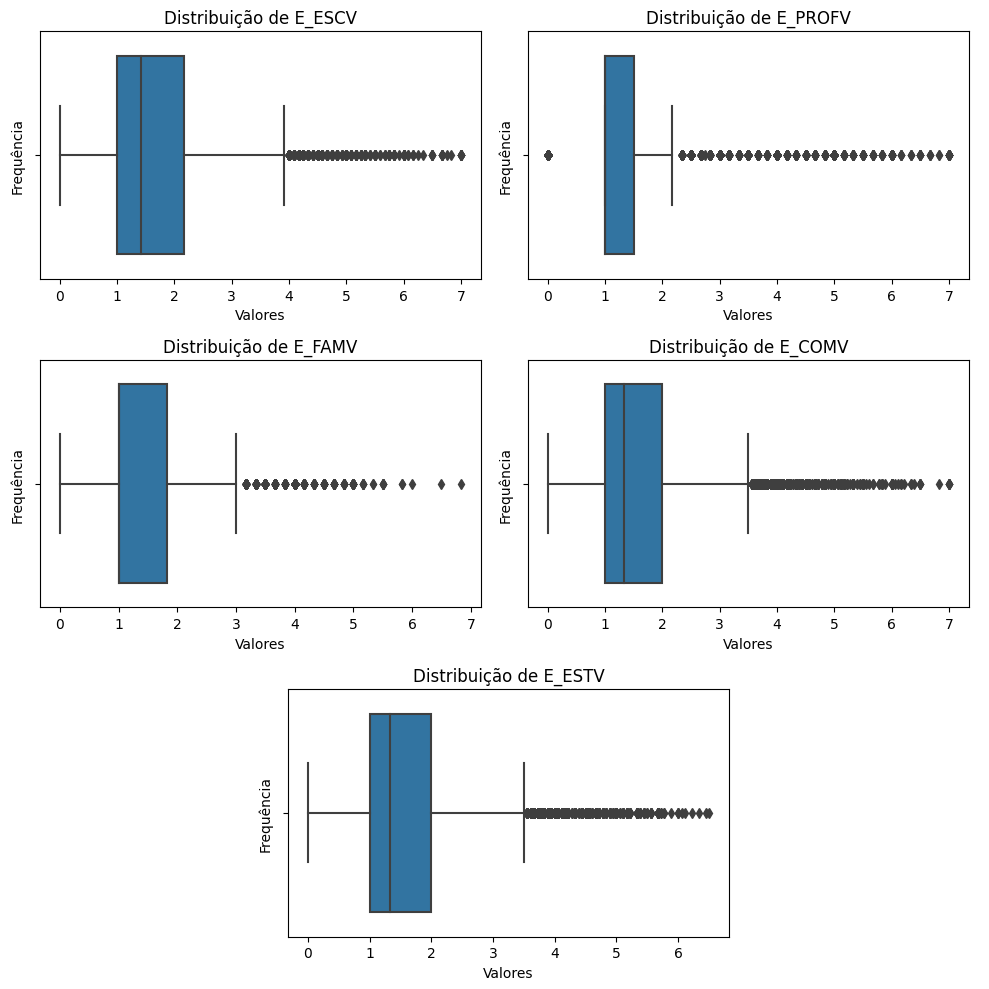
\includegraphics[width=0.8\textwidth]{Textuais/Imagens/Gráficos/boxplot_dim.png}
    \label{fig:box_plot_dimensoes}
    \fonte{\me{2023}}
\end{figure}



\begin{figure}[ht!]
    \centering
    \caption{Box Plot de distribuição de Fatores}
    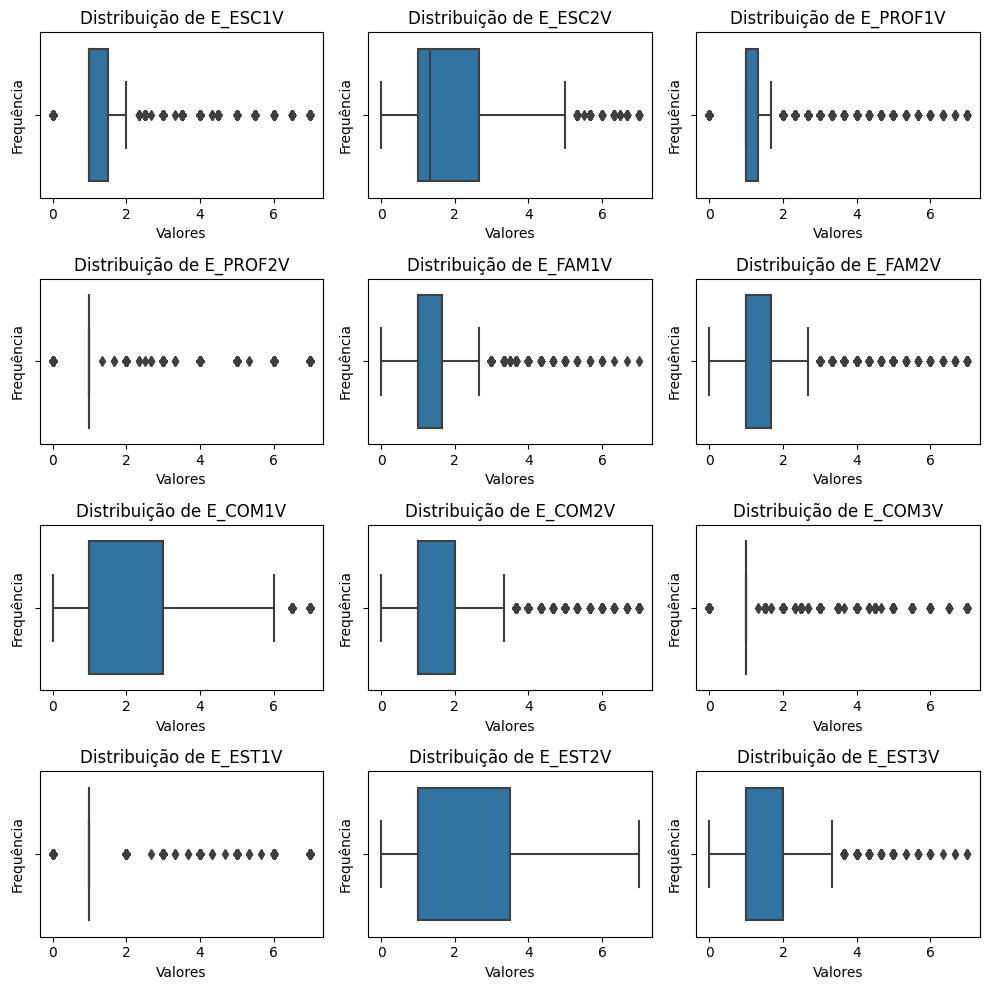
\includegraphics[width=0.8\textwidth]{Textuais/Imagens/Gráficos/boxplot_fat.png}
    \label{fig:box_plot_fatores}
    \fonte{\me{2023}}
\end{figure}




% As tabelas apresentam estatísticas descritivas relacionadas a fatores e dimensões de um questionário. Vamos analisar as conclusões possíveis com base nos números fornecidos:

% \textbf{Tabela de Estatísticas de Fatores:}

% \begin{enumerate}
%     \item E\_ESC1V tem uma média de aproximadamente 1.57, um desvio padrão de cerca de 1.19 e uma mediana de 1. Isso indica que a maioria das respostas está próxima da mediana, com uma dispersão moderada. Parece haver uma variedade razoável de respostas.
%     \item E\_ESC2V tem uma média de cerca de 1.93, um desvio padrão de aproximadamente 1.19 e uma mediana de 1.33. Isso sugere que as respostas estão distribuídas de forma um pouco mais ampla em comparação com E\_ESC1V, com uma mediana ligeiramente maior.
%     \item E\_PROF1V tem uma média de cerca de 1.39, um desvio padrão de aproximadamente 0.93 e uma mediana de 1. Parece haver menos dispersão nas respostas, com a maioria dos dados próximos à mediana.
%     \item E\_PROF2V tem uma média de aproximadamente 1.62, um desvio padrão de cerca de 1.60 e uma mediana de 1. A dispersão é alta, com uma mediana baixa, sugerindo uma variedade significativa de respostas.
%     \item E\_FAM1V tem uma média de cerca de 1.43, um desvio padrão de aproximadamente 0.79 e uma mediana de 1. As respostas parecem estar concentradas perto da mediana, com uma dispersão moderada.
%     \item E\_FAM2V tem uma média de aproximadamente 1.52, um desvio padrão de cerca de 1.06 e uma mediana de 1. A dispersão é moderada, e a mediana é próxima de 1, indicando que a maioria das respostas está nessa faixa.
%     \item E\_COM1V tem uma média de cerca de 2.01, um desvio padrão de aproximadamente 1.59 e uma mediana de 1. Isso indica uma dispersão considerável nas respostas, com uma mediana relativamente baixa.
%     \item E\_COM2V tem uma média de cerca de 1.60, um desvio padrão de aproximadamente 1.12 e uma mediana de 1. Parece haver uma variedade razoável nas respostas, com a maioria próxima à mediana.
%     \item E\_COM3V tem uma média de cerca de 1.35, um desvio padrão de aproximadamente 0.96 e uma mediana de 1. A dispersão é moderada, e a mediana está próxima de 1.
%     \item E\_EST1V tem uma média de cerca de 1.39, um desvio padrão de aproximadamente 1.22 e uma mediana de 1. A dispersão é moderada, com a maioria das respostas próximas à mediana.
%     \item E\_EST2V tem uma média de aproximadamente 2.03, um desvio padrão de cerca de 1.57 e uma mediana de 1. A dispersão é alta, e a mediana está próxima de 1.
%     \item E\_EST3V tem uma média de cerca de 1.53, um desvio padrão de aproximadamente 0.84 e uma mediana de 1. A dispersão é moderada, e a mediana está próxima de 1.
%     \end{enumerate}

    
% \textbf{Tabela de Estatísticas de Dimensões:}

% \begin{enumerate}
%     \item E\_ESCV tem uma média de aproximadamente 1.76, um desvio padrão de cerca de 0.96 e uma mediana de 1.42. Isso indica que a dimensão ``Estudante – Escola'' (E-ESC) tem uma dispersão moderada, com a maioria das respostas próxima à mediana.
    
%     \item E\_PROFV tem uma média de cerca de 1.50, um desvio padrão de aproximadamente 1.07 e uma mediana de 1. A dispersão é moderada, e a mediana está próxima de 1, sugerindo uma consistência nas respostas.
    
%     \item E\_FAMV tem uma média de aproximadamente 1.49, um desvio padrão de cerca de 0.78 e uma mediana de 1. A dimensão ``Estudante – Família'' (E-FAM) apresenta uma dispersão moderada, com a maioria das respostas próxima à mediana.
    
%     \item E\_COMV tem uma média de cerca de 1.68, um desvio padrão de aproximadamente 0.87 e uma mediana de 1.33. A dimensão ``Estudante – Comunidade'' (E-COM) tem uma dispersão moderada, com uma mediana acima de 1.
    
%     \item E\_ESTV tem uma média de aproximadamente 1.67, um desvio padrão de cerca de 0.86 e uma mediana de 1.33. A dimensão ``Estudante – Estudante'' (E-EST) apresenta uma dispersão moderada, com a maioria das respostas próxima à mediana. 
% \end{enumerate}
% Em resumo, as estatísticas fornecidas indicam a variabilidade nas respostas dos participantes do questionário, com algumas dimensões e fatores apresentando maior dispersão do que outras. É importante considerar esses resultados ao analisar os dados e as respostas do questionário em um contexto mais amplo.


%%%%%%%%%%%%%%%%%%%%%%%%%%%%%%%%%%%%%%%%%
%%%%%%%%%%%%%%%%%%%%%%%%%%%%%%%%%%%%%%%%%


A Figura \ref{fig:uf} apresenta o mapa temático do Brasil, colorido em diferentes tons que representam a quantidade de estudantes por estado que responderam ao questionário. A barra de cores à direita do mapa serve como uma legenda, indicando a relação entre as cores e o número de estudantes, com a escala variando do amarelo claro para números baixos até o vermelho escuro para números altos.

Há uma grande variação na quantidade de respostas por estado. Alguns estados, como o destacado em vermelho escuro no centro-norte do mapa, têm um número significativamente alto de estudantes respondentes, ultrapassando 5000. Isso sugere uma alta participação ou um foco particular na coleta de dados nesse estado. Por outro lado, há estados, especialmente no sul do país, que apresentam números baixos ou nulos, indicando uma possível falta de representatividade ou dificuldades na coleta de dados nessas áreas.

Além disso, o mapa fornece informações sobre onde podem estar concentradas as preocupações com a evasão, ou pelo menos onde mais estudantes foram alcançados para responder ao questionário. A heterogeneidade na distribuição dos números pode refletir diferenças no engajamento das secretarias de educação estaduais, na estrutura da pesquisa, ou até mesmo na própria incidência de evasão escolar.

\begin{figure}[ht!]
    \centering
    \caption{Distribuição das matrículas por estados}
    \includegraphics[width=\textwidth]{Textuais/Imagens/Gráficos/uf.png}
    \label{fig:uf}
\end{figure}

O gráfico da Figura \ref{fig:turmas} exibe a distribuição do número de estudantes que responderam ao questionário categorizados por ano escolar. Observa-se que a maior participação foi dos alunos do 6º ano, com 4912 respostas, seguida por uma ligeira diminuição para 4418 no 7º ano e uma redução mais acentuada para 4103 no 8º ano. O 9º ano apresenta um número ainda menor de respondentes, com 3506 alunos. Uma queda drástica é notada nos anos iniciais do ensino fundamental: apenas 61 estudantes do 5º ano, 59 do 1º ano, 23 do 3º ano, 18 do 2º ano e 9 do 4º ano participaram do questionário.

\begin{figure}[ht!]
    \centering
    \caption{Distribuição das matrículas por ano de turma do ensino fundamental}
    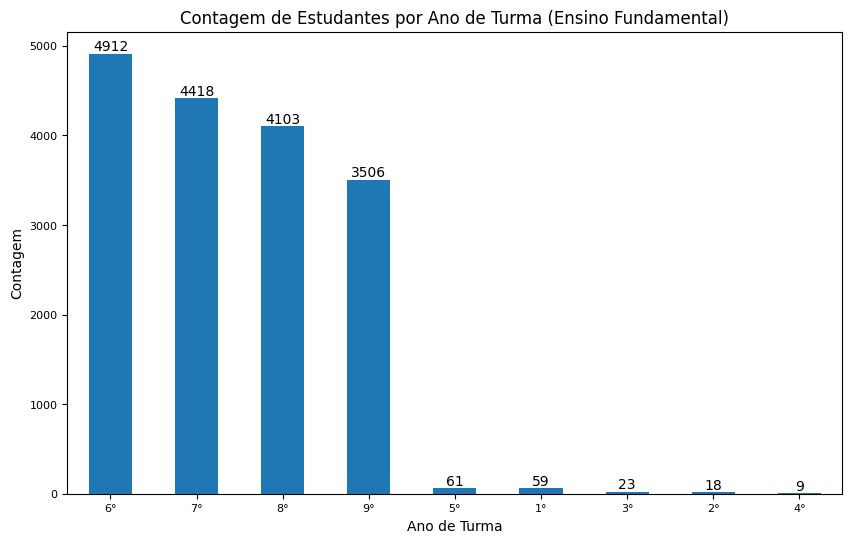
\includegraphics[width=0.8\textwidth]{Textuais/Imagens/Gráficos/turmas.png}
    \label{fig:turmas}
    \fonte{\me{2023}}
\end{figure}

O gráfico da Figura \ref{fig:sexo-porcent} é um gráfico de pizza que apresenta a distribuição por sexo dos estudantes que responderam o questionário. Do total de respondentes, 51,7\% são do sexo masculino e 48,3\% do sexo feminino. Isso indica uma distribuição quase equilibrada entre os gêneros, com uma ligeira predominância de respondentes masculinos. 

\begin{figure}[ht!]
    \centering
    \caption{Porcentagem do sexo dos estudantes}
    \includegraphics[width=0.6\textwidth]{Textuais/Imagens/Gráficos/sexo.png}
    \label{fig:sexo-porcent}
    \fonte{\me{2023}}
\end{figure}

% A renda familiar pode exercer uma influência significativa na permanência do estudante na escola devido a vários fatores. Estudantes de famílias com rendas mais baixas podem enfrentar dificuldades econômicas que os obrigam a priorizar o trabalho imediato em detrimento da educação continuada. Essa necessidade de contribuir para a renda da família pode levar à evasão escolar, já que o estudante pode ter que dedicar seu tempo a atividades remuneradas.

% Além disso, a limitação de recursos financeiros pode afetar a capacidade de uma família de pagar por materiais didáticos, uniformes, transporte e outras despesas educacionais. Isso pode resultar em uma experiência educacional de qualidade inferior, com menos apoio e recursos, o que, por sua vez, pode desmotivar o estudante e aumentar as chances de evasão escolar.

% Outro aspecto é o acesso a uma educação de qualidade. Em muitos casos, escolas localizadas em regiões de baixa renda podem estar superlotadas, mal equipadas e com menos oportunidades extracurriculares, o que pode afetar negativamente o engajamento e o desempenho do estudante. Estudantes de famílias com maior renda, em contraste, muitas vezes têm acesso a escolas privadas ou públicas bem financiadas, com uma ampla gama de programas de apoio, como tutoria e aconselhamento, que podem ajudar a mantê-los na escola.

% De acordo com um estudo realizado por Reardon et. al (2016)\nocite{reardon2019geography}, a renda familiar está fortemente associada às oportunidades educacionais e ao desempenho acadêmico. O estudo descobriu que, nos Estados Unidos, a lacuna de desempenho entre crianças de famílias de baixa renda e crianças de famílias de alta renda é significativa e tem aumentado ao longo do tempo. As crianças de famílias de baixa renda têm menos acesso a recursos educacionais, como escolas de alta qualidade, professores experientes e programas extracurriculares, o que pode afetar negativamente suas expectativas e aspirações educacionais. Além disso, as famílias de baixa renda podem ter menos recursos financeiros para investir na educação de seus filhos, o que pode limitar suas oportunidades educacionais a longo prazo.


% Portanto, é possível afirmar que a renda familiar influencia diretamente as expectativas educacionais e os resultados a longo prazo, uma vez que as famílias com maior renda geralmente têm mais recursos para apoiar a educação de seus filhos, enquanto as famílias de baixa renda podem enfrentar desafios financeiros e ter menos acesso a recursos educacionais.

% Políticas e programas focados em aumentar o apoio financeiro para famílias de baixa renda, fornecer recursos educacionais adicionais, e criar oportunidades de ensino pós-escolar podem ser cruciais para reduzir as taxas de evasão escolar e promover a igualdade educacional.

Desta forma, o gráfico da Figura \ref{fig:renda_fam} apresenta a distribuição de renda das famílias dos estudantes respondentes. A maior concentração de estudantes, 8.735, tem uma renda familiar de até 1 salário mínimo (até R\$ 1.320). A segunda maior faixa, com 5.222 estudantes, situa-se entre 1 a 3 salários mínimos (de R\$ 1.320 até R\$ 3.960). Uma parcela considerável, 2.130 estudantes, indicou não possuir nenhuma renda. A faixa de 4 a 6 salários mínimos (de R\$ 5.280 até R\$ 7.920) é composta por 816 estudantes. Observa-se uma diminuição progressiva na quantidade de estudantes à medida que a renda familiar aumenta: 139 estudantes pertencem à faixa de 7 a 9 salários mínimos (de R\$ 9.240 até R\$ 11.880), e apenas 67 estudantes têm uma renda familiar acima de 9 salários mínimos (mais de R\$ 11.880). Esse perfil sugere que a maioria dos estudantes que participaram do questionário provém de famílias com menor renda.


\begin{figure}[ht!]
    \centering
    \caption{Distribuição de renda da família dos estudantes}
    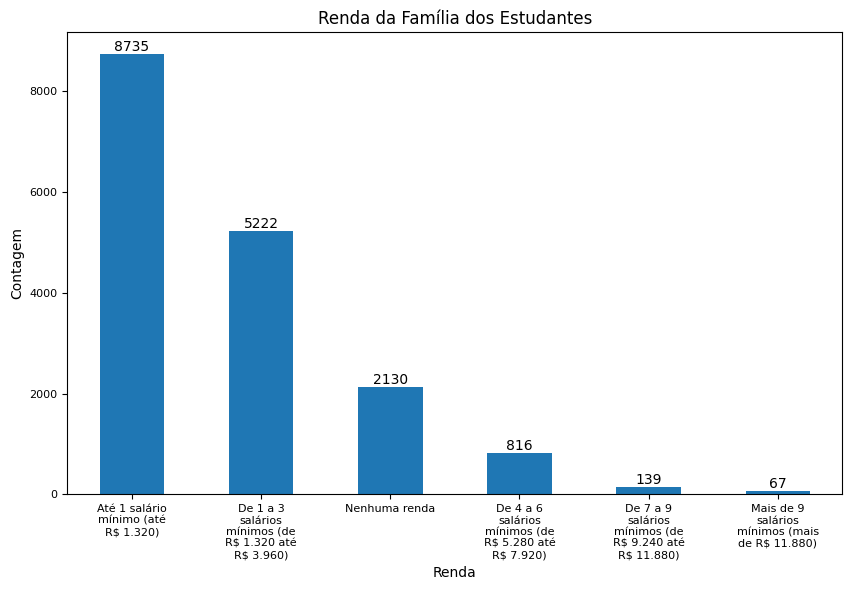
\includegraphics[width=0.8\textwidth]{Textuais/Imagens/Gráficos/renda_fam.png}
    \label{fig:renda_fam}
    \fonte{\me{2023}}
\end{figure}


% A oferta de Atendimento Educacional Especializado (AEE) é uma prática inclusiva essencial que visa atender às necessidades específicas de estudantes com deficiência, transtornos globais do desenvolvimento ou altas habilidades/superdotação. Quando as escolas fornecem esse tipo de suporte especializado, elas não apenas ajudam a nivelar o campo de jogo educacional para esses alunos, mas também promovem uma cultura de inclusão e igualdade. A presença de serviços de AEE pode aumentar significativamente as chances de retenção dos estudantes na escola, uma vez que se sentem apoiados em suas necessidades educacionais particulares e, consequentemente, mais engajados e motivados para continuar seus estudos.

% Por outro lado, as atividades complementares, que podem incluir clubes, esportes, música, arte, e outras experiências enriquecedoras, desempenham um papel vital na educação holística dos alunos. Essas atividades são fundamentais para o desenvolvimento de habilidades sociais, emocionais e cognitivas. Alunos que participam dessas atividades tendem a desenvolver um senso de pertencimento e compromisso com sua comunidade escolar. A disponibilidade de tais programas pode influenciar positivamente a decisão de um aluno de permanecer na escola, pois eles proporcionam uma saída para a expressão criativa, alívio do estresse e oportunidades para amizades e mentorias. Além disso, as atividades complementares aumentam frequentemente o engajamento dos alunos com o ambiente escolar e podem melhorar o desempenho acadêmico, tornando a experiência educacional mais atraente e valiosa.

% A combinação dessas ofertas indica que a escola está buscando atender a uma gama diversificada de necessidades dos alunos, tanto educacionais quanto de desenvolvimento pessoal. Tais esforços multidimensionais são fundamentais para a retenção de estudantes, pois eles se sentem compreendidos e atendidos em suas demandas individuais. Ao considerar o aspecto multidisciplinar do desenvolvimento do estudante e suas variadas necessidades, a escola pode reduzir os índices de evasão e fomentar uma comunidade escolar mais integrada e resiliente.

O gráfico da Figura \ref{fig:outras_ofertas} apresenta a distribuição de frequência de estudantes em relação a três categorias distintas de Outras Ofertas Educacionais. Observa-se que a maior frequência está na categoria ``Atendimento Educacional Especializado'', com 5646 estudantes. Isso indica que esta é a oferta educacional mais acessada ou necessitada pelo grupo de estudantes que respondeu ao questionário. Em seguida, temos a ``Atividade Complementar'', com 1615 estudantes, demonstrando uma procura ou necessidade significativamente menor em comparação à primeira. Por fim, a categoria ``Atendimento Educacional Especializado, Atividade Complementar'' registra 1212 estudantes, sugerindo que há um número considerável de estudantes que necessitam ou acessam uma combinação das ofertas. 

\begin{figure}[ht!]
    \centering
    \caption{Número de estudantes que estão matriculados em instituições que possuem ofertas educacionais diferenciadas}
    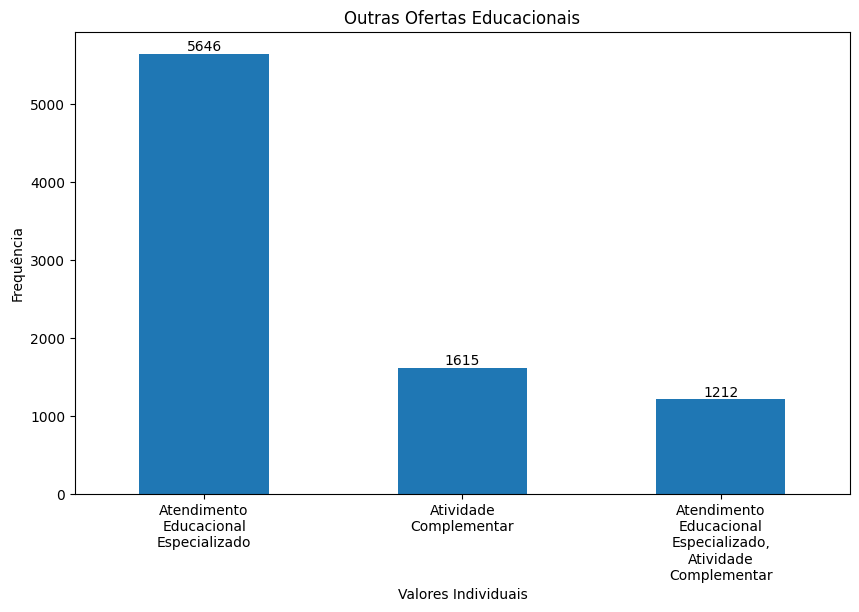
\includegraphics[width=0.8\textwidth]{Textuais/Imagens/Gráficos/outras_ofertas_educacionais.png}
    \label{fig:outras_ofertas}
    \fonte{\me{2023}}
\end{figure}



% A localização das escolas, seja em áreas rurais ou urbanas, pode influenciar significativa na permanência dos estudantes na escola. Em áreas urbanas, os estudantes costumam ter acesso a uma gama mais ampla de recursos educacionais, como tecnologia mais avançada, maior número de professores qualificados, e uma variedade maior de programas extracurriculares e de apoio ao aluno. Esses fatores podem contribuir para uma maior taxa de retenção de alunos, já que eles têm mais oportunidades de engajamento e aprendizado. Além disso, escolas urbanas muitas vezes estão mais próximas dos serviços de apoio ao estudante, como bibliotecas públicas e centros de tutoria \cite{santos2012estudo}. 


% Por outro lado, escolas localizadas em áreas rurais podem enfrentar desafios distintos que impactam a permanência do estudante. O acesso limitado a recursos, como Internet de alta velocidade e materiais didáticos atualizados, pode afetar a qualidade da educação. Distâncias maiores para se percorrer até a escola e a falta de transporte público adequado são problemas comuns que podem levar a altas taxas de evasão, pois tornam o simples ato de chegar à escola um desafio. Além disso, em muitas comunidades rurais, pode haver uma expectativa maior de que os jovens contribuam para o trabalho familiar, o que pode priorizar as necessidades de trabalho em detrimento da educação formal.

% Outra consideração é o impacto econômico e cultural das áreas rurais e urbanas. Em regiões rurais, pode haver menos incentivo para a educação de longo prazo se as oportunidades de emprego local forem limitadas ou se valorizarem mais as habilidades práticas adquiridas fora do ambiente escolar. Em contrapartida, áreas urbanas tendem a oferecer uma maior variedade de oportunidades profissionais que requerem educação formal, incentivando os estudantes a concluírem seus estudos.

% De acordo com o Observatório da Criança e do Adolescente, a média de horas-aula no Ensino Fundamental varia de acordo com a localização da escola, sendo que a média de horas-aula expressa o tempo médio de permanência dos alunos na escola segundo a localização (urbana ou rural) do estabelecimento de ensino. A média apresentada é ponderada por fator que deriva das relações entre: a matrícula na data de referência do Censo Escolar, a série, os grupos de séries e níveis de ensino. Para este indicador são consideradas apenas as turmas de escolarização na modalidade Regular \footnote{https://observatoriocrianca.org.br/cenario-infancia/temas/ensino-fundamental/883-media-de-horas-aula-no-ensino-fundamental-segundo-localizacao-urbana-e-rural?filters=1,1385}.
% Além disso, a quantidade de horas-aula modifica conforme a localidade da escola, apresentando um número menor em escolas de área rural.

% Por fim, políticas públicas e investimentos em educação podem variar consideravelmente entre áreas rurais e urbanas, afetando diretamente a permanência dos estudantes na escola. Iniciativas para melhorar a infraestrutura escolar, oferecer transporte aos estudantes e programas de incentivo à permanência na escola são essenciais para garantir que a localização geográfica não seja uma barreira à educação. Reconhecer e abordar essas diferenças é fundamental para qualquer estratégia que vise diminuir a evasão escolar e promover a igualdade de acesso à educação de qualidade para todos os estudantes.


Já o gráfico da Figura \ref{fig:localizacao} mostra a localização das escolas de acordo com as respostas dos estudantes. De acordo com as informações fornecidas, 59,2\% dos estudantes estão em escolas localizadas em áreas urbanas, enquanto os restantes 40,8\% estão em escolas situadas em áreas rurais. Isso indica uma distribuição relativamente equilibrada entre as localizações das escolas dos respondentes, com uma ligeira predominância de estudantes em zonas urbanas. Na Tabela \ref{tab:localizacao_escolas_estado}, foi realizada a separação do número de escolas e sua localização por cada estado, querendo analisar melhor da distribuição de escolas rurais e urbanas no âmbito nacional. É possível observar que a maioria dos estados possui maior concentração urbana, exceto pelos estados de Alagoas, Bahia, Maranhão, Pará e Rio Grande do Norte.

\begin{figure}[ht!]
    \centering
    
    \caption{Porcentagem da localização das escolas}
    \includegraphics[width=0.6\textwidth]{Textuais/Imagens/Gráficos/localizacao.png}
    \label{fig:localizacao}
    \fonte{\me{2023}}
\end{figure}

\begin{table}[ht!]
\centering
\caption{Localização das escolas dividida por estado}
\label{tab:localizacao_escolas_estado}
\resizebox{\textwidth}{!}{%
\begin{tabular}{|c|c|c|c|c|c|c|c|c|c|c|c|c|c|c|c|c|c|c|c|c|c|}
\hline
\textbf{UF}                               & AL & AM & BA & CE & DF & ES & GO & MA & MG & MS & PA & PB & PE & PI & RJ & RN & RR & SC & SE & SP & TO \\ \hline
\textbf{Rural}                            & 4  & 1  & 17 & 7  & 0  & 0  & 1  & 14 & 5  & 0  & 68 & 1  & 1  & 5  & 0  & 6  & 0  & 0  & 1  & 1  & 15 \\ \hline
\textbf{Urbana} & 3  & 1  & 9  & 12 & 1  & 1  & 28 & 7  & 9  & 2  & 33 & 3  & 1  & 11 & 2  & 2  & 4  & 1  & 4  & 4  & 23 \\ \hline
\end{tabular}%
}
\fonte{\me{2023}}
\end{table}

% A localidade de uma escola pode exercer um papel crucial na permanência do estudante na instituição. Em áreas de assentamento, por exemplo, os estudantes podem enfrentar desafios como acesso limitado ao transporte, recursos educacionais escassos ou infraestrutura inadequada, o que pode contribuir para altas taxas de evasão escolar. Estes assentamentos estão frequentemente situados em locais remotos, onde as escolas podem lutar para atrair e reter professores qualificados, e os alunos podem ter que viajar longas distâncias para frequentar as aulas, o que pode ser um impedimento significativo à regularidade da frequência escolar.

% Em áreas remanescentes de quilombos, as escolas estão muitas vezes inseridas em comunidades com raízes históricas e culturais. Embora isso possa fornecer um ambiente de aprendizado rico culturalmente, também pode haver desafios devido ao isolamento geográfico e à falta de recursos. Questões como a relevância cultural do currículo e a sensibilidade dos professores às tradições locais podem influenciar a decisão do estudante de continuar na escola. Nas terras indígenas, a situação é muitas vezes mais complexa, pois envolve a preservação da língua e da cultura indígenas, além dos desafios de infraestrutura e acessibilidade. A educação nessas áreas pode ser dificultada por políticas governamentais inadequadas ou pela falta de material didático que incorpore a língua e a cultura indígenas. A relevância cultural do ensino é um fator determinante para a permanência do estudante, e a falta dela pode levar à desmotivação e ao abandono escolar.

O gráfico apresentado na Figura \ref{fig:localidades} é um diagrama de barras que exibe a distribuição de escolas por tipos de localidades diferenciadas. Três categorias são exibidas: ``Área de assentamento'', ``Área remanescente de quilombos'' e ``Terra indígena''. A maior contagem de escolas, com um total de 25, encontra-se em ``Área de assentamento''. Em segundo lugar, com 8 escolas, estão as ``Áreas remanescentes de quilombos''. Por fim, ``Terra indígena'' apresenta 4 escolas. Considerando o gráfico da Figura \ref{fig:localidades_brasil}, feito com os dados do Novo Censo Educacional exclusivos do ano de 2022\footnote{https://www.gov.br/inep/pt-br/acesso-a-informacao/dados-abertos/microdados/censo-escolar}, nota-se que a proporcionalidade das escolas pesquisadas que estão em localizações diferenciadas não foi igual na pesquisa do SAP. Sabendo que foram pesquisadas 224.649 escolas no Censo, os resultados mostram que a porcentagem de escolas com localizações em área de assentamento, terras indígenas e áreas remanescentes de quilombos era 2.03\%, 1.5\% e 1.14\%, respectivamente. Já no SAP, essas mesmas categorias possuem porcentagens de 8.11\%, 1.29\% e 2.59\%; ou seja, o dobro para remanescentes.

\begin{figure}[ht!]
    \centering
    \caption{Localização diferenciada das escolas}
    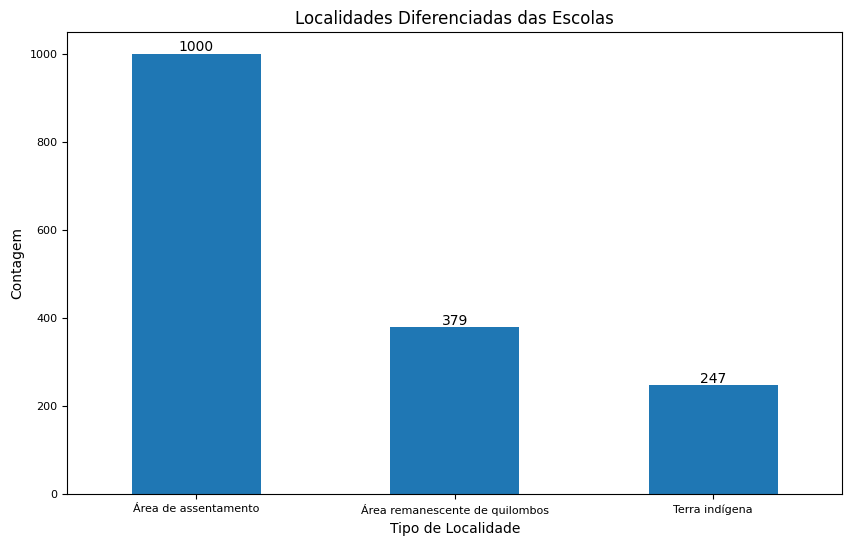
\includegraphics[width=0.8\textwidth]{Textuais/Imagens/Gráficos/localidadesdifer.png}
    \label{fig:localidades}
    \fonte{\me{2023}}
\end{figure}

\begin{figure}[ht!]
    \centering
    \caption{Localização diferenciada das escolas brasileiras no ano de 2022}
    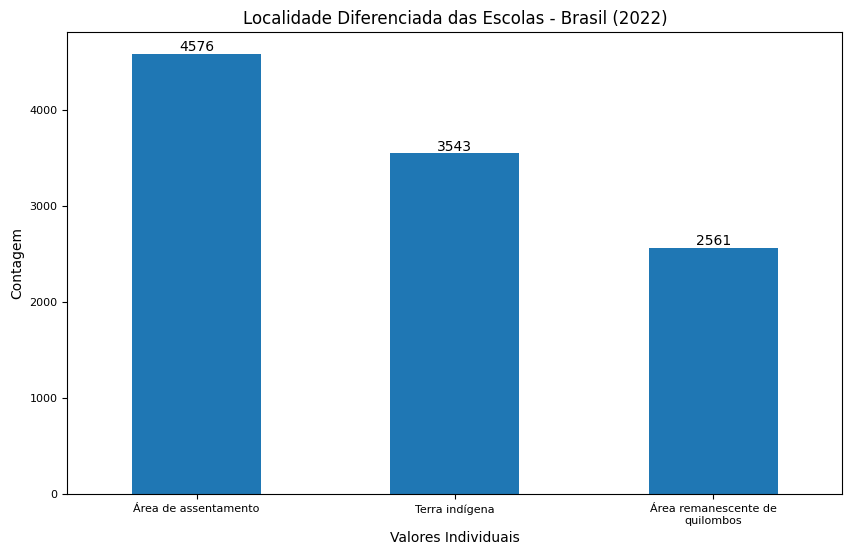
\includegraphics[width=0.8\textwidth]{Textuais/Imagens/Gráficos/localidadesdifer_brasil.png}
    \label{fig:localidades_brasil}
    \fonte{\me{2023}}
\end{figure}

% A faixa do número de matrículas em uma escola pode ter diversas implicações na permanência dos estudantes, influenciando diretamente a qualidade da educação e o ambiente escolar. Em escolas com um número elevado de matrículas, que muitas vezes correspondem a escolas de maior porte, pode haver acesso a mais recursos, como bibliotecas mais amplas, maior variedade de atividades extracurriculares e infraestrutura esportiva. Isso pode aumentar o engajamento dos alunos e diminuir as chances de evasão. No entanto, o grande número de estudantes pode também levar a uma menor atenção individual por parte dos professores e funcionários, o que pode afetar negativamente os alunos que necessitam de maior suporte pedagógico. Por outro lado, escolas com poucas matrículas podem proporcionar um ambiente mais acolhedor e personalizado, com maior proximidade entre alunos e professores. Nesses ambientes, os educadores podem acompanhar mais de perto o progresso e as dificuldades de cada aluno, o que pode ser decisivo na prevenção da evasão escolar. No entanto, essas escolas podem enfrentar limitações de recursos, o que poderia afetar a oferta de cursos e atividades e, por conseguinte, o interesse dos alunos em permanecer na escola.

O gráfico da Figura \ref{fig:faixa_num} ilustra a distribuição do número de matrículas das escolas. O eixo horizontal representa diferentes faixas de número de matrículas, enquanto o eixo vertical indica a contagem de escolas em cada faixa. A maior concentração de escolas se encontra na faixa de ``Entre 51 e 200'' matrículas, com um total de 92 escolas. Segue-se a faixa de ``Entre 501 e 1000'' matrículas com 67 escolas, e ``Mais de 1000'' com 21 escolas. Por fim, o número de escolas com ``Até 50'' matrículas é o mais baixo, com apenas 5 instituições. Este gráfico traz o entendimento da distribuição do tamanho das escolas entre os estudantes que participaram do questionário, o que pode fornecer uma visão mais completa para a análise da evasão escolar.

\begin{figure}[ht!]
    \centering
    \caption{Faixa do número de matrículas das escolas}
    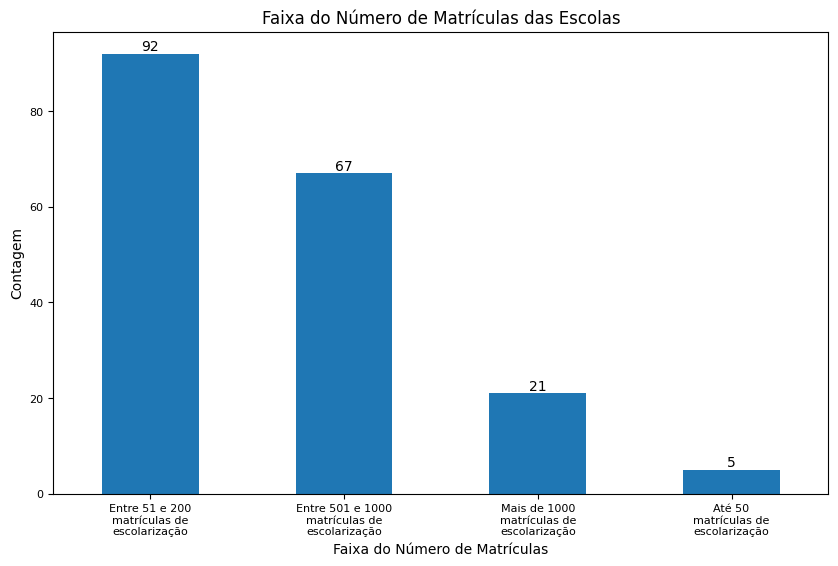
\includegraphics[width=0.8\textwidth]{Textuais/Imagens/Gráficos/faixanumamatr.png}
    \label{fig:faixa_num}
    \fonte{\me{2023}}
\end{figure}

A etnia dos estudantes está relacionada a uma complexa teia de fatores sociais, econômicos e culturais. Estudantes identificados como pardos, pretos, indígenas e amarelos podem enfrentar desafios adicionais que afetam sua jornada educacional. Questões como disparidades socioeconômicas, preconceito e racismo estrutural podem influenciar negativamente a experiência desses estudantes nas instituições de ensino \cite{heringer2018democratizaccao}. O gráfico apresentado na Figura \ref{fig:etnia} mostra a distribuição étnica dos estudantes que responderam o questionário. A categoria com maior número de estudantes é a ``Pardo/a'', com 12.450 respostas, seguida consideravelmente pela categoria ``Branco/a'' com 2.443 estudantes. A terceira categoria mais numerosa é a ``Preto/a'', representando 1.758 estudantes. Em menor quantidade, aparecem os estudantes que se identificam como ``Indígena'', somando 290, e a categoria ``Amarelo/a (Origem Asiática)'' com 168 estudantes. A representação visual destes dados permite uma compreensão imediata das proporções relativas de cada grupo étnico dentro do conjunto dos respondentes, destacando a predominância do grupo ``Pardo/a'' neste contexto específico.

Observando os microdados das etnias do Censo da Educação Básica do ano de 2022, apresentados na Figura \ref{fig:etnia-brasil}, nota-se que proporcionalmente, os números de representatividade das etnias são muito semelhantes, com a exceção dos declarados brancos e dos estudantes não declarados, que no Censo são o terceiro maior grupo, mas que no SAP não é bem uma categoria existente, indicando que todos os 17110 respondentes declararam suas etnias.

% Para estudantes pardos e pretos, por exemplo, a marginalização histórica e contínua pode levar a menores investimentos em suas comunidades e escolas, resultando em acesso desigual a recursos educacionais de qualidade. Além disso, o racismo e a discriminação podem criar ambientes escolares hostis, reduzindo o senso de pertencimento e segurança desses alunos, o que pode aumentar as taxas de evasão.

% De acordo com a pesquisa realizada pelo Observatório de Educação do Instituto Unibanco\footnote{https://observatoriodeeducacao.institutounibanco.org.br/em-debate/desigualdade-racial-na-educacao}, a marginalização histórica e contínua pode levar a menores investimentos em comunidades e escolas, resultando em acesso desigual a recursos educacionais de qualidade para estudantes pardos e pretos. Além disso, o racismo e a discriminação podem criar ambientes escolares hostis, reduzindo o senso de pertencimento e segurança desses alunos, o que pode aumentar as taxas de evasão

% Estudantes indígenas muitas vezes enfrentam barreiras ainda maiores, como a distância física de suas comunidades para as escolas, a falta de materiais didáticos que respeitem e reflitam suas culturas e línguas, e um modelo educacional que frequentemente não leva em conta suas tradições e saberes.

% Conforme o ensaio ``O passado e o futuro da educação indígena: barreiras e soluções'' do \textit{Indigenous Brazil}\footnote{https://commons.princeton.edu/indigenous-brazil/outros-textos/o-passado-e-o-futuro-da-educacao-indigena-barreiras-e-solucoes/}, estudantes indígenas enfrentam barreiras ainda maiores, como a distância física de suas comunidades para as escolas, a falta de materiais didáticos que respeitem e reflitam suas culturas e línguas, e um modelo educacional que frequentemente não leva em conta suas tradições e saberes

% Por outro lado, estudantes amarelos, que podem incluir descendentes de imigrantes asiáticos, podem experimentar estereótipos tanto positivos quanto negativos que afetam suas experiências educacionais. Embora muitas vezes sejam vistos sob a ``lente do modelo minoritário'', que pressupõe um alto desempenho acadêmico, eles também podem enfrentar isolamento cultural e racismo.

% Estudantes brancos, em muitos contextos, podem ter vantagens devido a privilégios estruturais que lhes concedem melhor acesso a escolas de alta qualidade, materiais didáticos e oportunidades extracurriculares. Contudo, isso não significa que estudantes brancos não enfrentem desafios que possam influenciar sua permanência na escola; fatores como condição socioeconômica e outras questões individuais ou familiares também são relevantes.



\begin{figure}[ht!]
    \centering
    \caption{Etnias dos estudantes que responderam o IAFREE}
    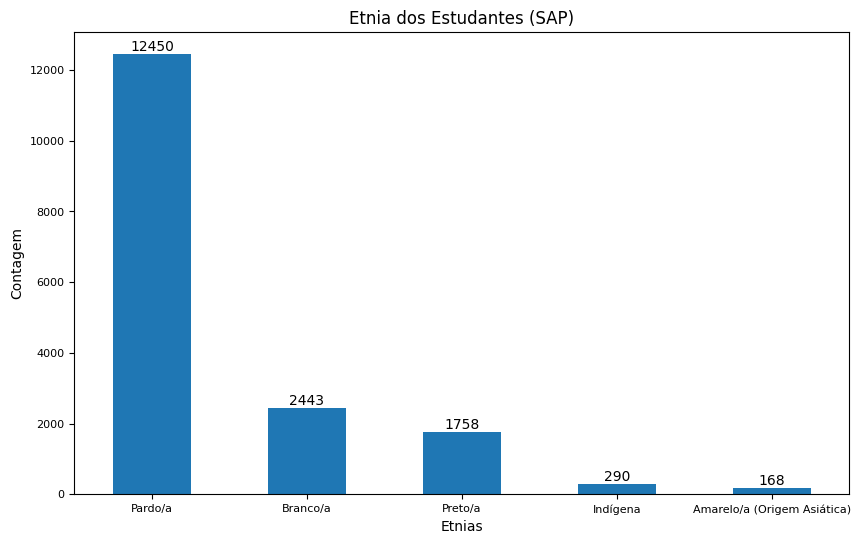
\includegraphics[width=0.8\textwidth]{Textuais/Imagens/Gráficos/etnia.png}
    \label{fig:etnia}
    \fonte{\me{2023}}
\end{figure}

\begin{figure}[ht!]
    \centering
    \caption{Etnias dos estudantes - Censo 2022}
    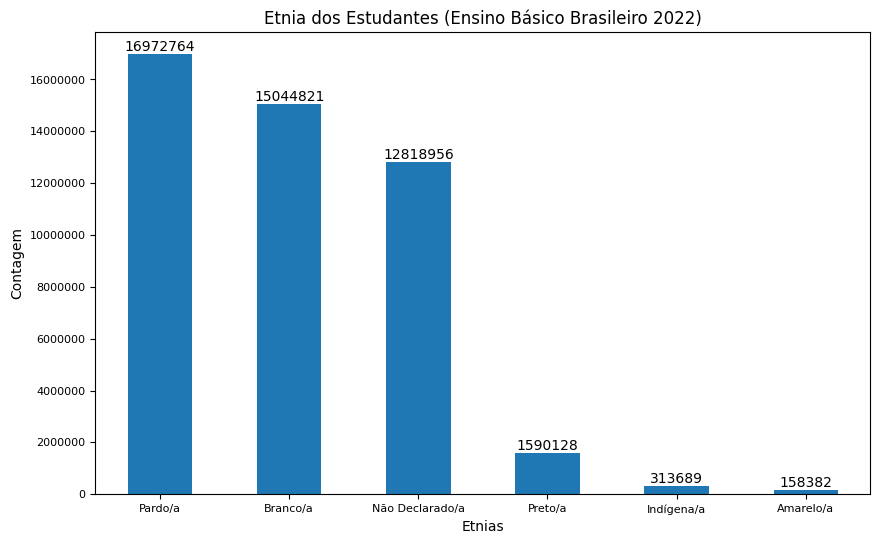
\includegraphics[width=0.8\textwidth]{Textuais/Imagens/Gráficos/etnia_brasil.png}
    \label{fig:etnia-brasil}
    \fonte{\me{2023}}
\end{figure}


A dependência administrativa das escolas pode exercer uma influência na permanência do estudante, escolas municipais e estaduais, muitas vezes, diferem em termos de recursos financeiros, infraestrutura, qualidade do ensino e programas pedagógicos, o que pode afetar diretamente a taxa de evasão escolar. Portanto, a dependência administrativa é apenas um dos muitos fatores que podem influenciar a permanência do estudante na escola. O gráfico da Figura \ref{fig:dependecia} é um gráfico de pizza que ilustra a ``Dependência Administrativa das Escolas'', que destaca a divisão entre escolas municipais e estaduais no contexto geral da pesquisa. Do total, uma maior porção, exatamente 62,3\%, representa as escolas municipais, enquanto as escolas estaduais compõem os restantes 37,7\%. A predominância das escolas municipais pode sugerir uma maior participação ou prevalência destas na amostra de estudantes que responderam ao questionário. Para ter um melhor comparativo entre os estados, a Tabela \ref{tab:dep_adm_escolas_estado} mostra a divisão entre os estados, notando-se uma forte representatividade das escolas municipais na maioria dos estados, com exceção de Goías, Minas Gerais, Roraima, São Paulo e Tocantins.



% Escolas municipais, geridas pelos governos locais, podem ter melhor capacidade de atender às necessidades específicas da sua comunidade imediata. Elas podem oferecer programas que são mais alinhados com o contexto local e, com a proximidade administrativa, podem ser mais receptivas às sugestões e necessidades dos estudantes e pais. Contudo, dependendo do município, essas escolas podem sofrer com a falta de recursos, o que pode levar à infraestrutura precária e à falta de materiais didáticos e professores qualificados, contribuindo para a evasão escolar.

% Por outro lado, as escolas estaduais, gerenciadas pelos governos estaduais, podem ter acesso a um orçamento maior e a uma estrutura administrativa mais ampla. Isso pode resultar em melhor infraestrutura e recursos, programas de formação continuada para professores e projetos educacionais de maior alcance. No entanto, a gestão centralizada pode não ser tão sensível às necessidades locais e, às vezes, pode resultar em políticas genéricas que não atendem às particularidades de cada comunidade.

% Além disso, a formação e a retenção de professores podem variar substancialmente entre as escolas municipais e estaduais, influenciando a qualidade do ensino e, consequentemente, a permanência dos alunos. Professores mais qualificados e bem remunerados podem ser mais prevalentes em escolas estaduais, resultando em melhores resultados educacionais e menor evasão.

% Por fim, a evasão escolar pode ser impactada pela governança e pelas políticas educacionais em vigor em cada nível administrativo. Programas de intervenção focados na redução da evasão escolar, como o acompanhamento individualizado de estudantes em risco, investimentos em aconselhamento e apoio psicológico, bem como a implementação de métodos pedagógicos inovadores, podem ser adotados de maneira diferente pelas escolas municipais e estaduais.



\begin{figure}[ht!]
    \centering
    \caption{Taxa de porcentagens das dependências administrativas das escolas}
    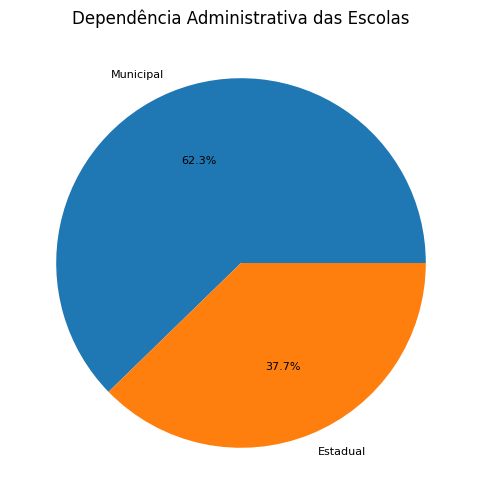
\includegraphics[width=0.5\textwidth]{Textuais/Imagens/Gráficos/dependenciaadm.png}
    \label{fig:dependecia}
    \fonte{\me{2023}}
\end{figure}

\begin{table}[ht!]
\centering
\caption{Dependência administrativa das escolas dividida por estado}
\label{tab:dep_adm_escolas_estado}
\resizebox{\textwidth}{!}{%
\begin{tabular}{|c|c|c|c|c|c|c|c|c|c|c|c|c|c|c|c|c|c|c|c|c|c|}
\hline
\textbf{UF}        & AL & AM & BA & CE & DF & ES & GO & MA & MG & MS & PA & PB & PE & PI & RJ & RN & RR & SC & SE & SP & TO \\ \hline
\textbf{Estadual}  & 0  & 1  & 0  & 0  & 1  & 0  & 29 & 0  & 13 & 1  & 16 & 0  & 0  & 0  & 0  & 0  & 4  & 0  & 2  & 5  & 27 \\ \hline
\textbf{Municipal} & 7  & 1  & 26 & 19 & 0  & 1  & 0  & 21 & 1  & 1  & 85 & 4  & 2  & 16 & 2  & 8  & 0  & 1  & 3  & 0  & 11 \\ \hline
\end{tabular}%
}
\fonte{\me{2023}}
\end{table}



%%%%%%%%%%%%%%%%%%%%%%%%%%%%%%%%%%%%%%
%%%%%%%%%%%%%%%%%%%%%%%%%%%%%%%%%%%%%%
%%%%%%%%%%%%%%%%%%%%%%%%%%%%%%%%%%%%%%
%%%%%%%%%%%%%%%%%%%%%%%%%%%%%%%%%%%%%%


%%%%%%%%%%%%%%%%%%%%%%%%%%%%%%%%%%%%%%
\chapter{Análises estatísticas}

% \textcolor{red}{Profs, eu ainda não consegui escrever sobre isso, mas a minha intenção nesse capítulo é correlacionar quais variáveis tem mais impacto em cada uma das visualizações, focando em quais delas seriam mais preditíveis segundo a análise dos algoritmos do capitulo anterior, conseguindo fechar na conclusão qual seria a melhor métrica possível pro SAP}

Para se compreender a relevância estatística significativa tanto das dimensões quanto dos fatores nas possíveis influências das variáveis socioeconômicas observadas no Capítulo \ref{cap:analises-sap}, foi decidido traçar o valor p (ou p-valor) para cada uma delas. Essa é uma medida estatística que ajuda a avaliar a significância estatística de um resultado em um teste de hipótese, então o valor p é a probabilidade de observar um resultado igual ou mais extremo do que o observado, sob a suposição de que a hipótese nula é verdadeira.

Para se calcular o valor p, é necessário primeiro traçar qual é a Hipótese Nula (H0), que é uma afirmação que assume que não há efeito ou diferença significativa; o valor p é usado para testar a validade da hipótese nula. Depois, traça-se a Hipótese Alternativa (H1), que é a afirmação que se deseja testar, sugerindo que existe uma diferença ou efeito significativo. Um valor p baixo (geralmente < 0,05) sugere que os resultados observados são improváveis de ocorrer sob a hipótese nula, levando à rejeição da hipótese nula. Um valor p alto indica que os resultados observados são plausíveis sob a hipótese nula, e não há evidências suficientes para rejeitá-la. Caso o valor p for menor que o nível de significância, rejeitamos a hipótese nula. Se o valor p for maior, não temos evidências suficientes para rejeitar a hipótese nula.

Para analisar essas relações das variáveis socioeconômicas com as dimensões e fatores, as Tabelas \ref{tab:pvalor_dimensao} e \ref{tab:pvalor_fatores} foram construídas. Elas apresentam os p-valores em destaque para todos os resultados menores que $0.05$, ou seja, os resultados com significância estatística. Então, analisando a Tabela \ref{tab:pvalor_dimensao}, é notável que os valores de p variam significativamente entre as diferentes variáveis, indicando que a associação entre essas variáveis e as dimensões ou fatores não é uniforme. Observa-se que, para a dimensão E\_ESCV (Estudante-Escola), o sexo não apresenta uma associação significativa, enquanto o ``porte\_da\_escola'' e ``id\_renda\_familiar'' mostram uma associação forte com p-valores muito baixos. Isso sugere que características como o tamanho da escola e a renda familiar têm um impacto mais significativo na dimensão relacionada à escola. No contexto da dimensão E\_PROFV (Profissionais da Escola), o sexo tem um p-valor muito baixo, indicando uma associação significativa. Além disso, ``ano\_turma'' e ``outras\_ofertas\_educacionais'' também apresentam p-valores baixos, sugerindo uma associação considerável com essa dimensão.

Para a dimensão E\_FAMV (Estudante-Família), vários fatores, como ``sexo'', ``uf'', ``localizacao'', ``ano\_turma'', ``localidade\_diferenciada'', ``dependencia\_administrativa'', ``id\_raca\_etnia'', ``porte\_da\_escola'', ``outras\_ofertas\_educacionais'' e ``id\_renda\_familiar'', mostram p-valores muito baixos. Isso sugere que esses fatores estão fortemente associados à dimensão relacionada à família. Ao examinar a dimensão E\_COMV (Estudante-Comunidade), quase todas as variáveis têm p-valores muito baixos, indicando associações significativas. Notavelmente, ``sexo'' e ``ano\_turma'' têm p-valores mais elevados, sugerindo uma menor associação com essa dimensão. Por fim, para a dimensão E\_ESTV (Estudante-Estudante), vários fatores apresentam p-valores altos, indicando uma associação menos significativa. ``sexo'', ``localizacao'', ``ano\_turma'', ``localidade\_diferenciada'', ``dependencia\_administrativa'', ``id\_raca\_etnia'', ``porte\_da\_escola'', ``outras\_ofertas\_educacionais'' e ``id\_renda\_familiar'' têm p-valores relativamente altos, sugerindo que esses fatores podem ter uma influência menos acentuada na dimensão do estudante. 

\begin{table}[ht!]
    \centering
    \caption{P Valor relacionado às Dimensões}
    \resizebox{\textwidth}{!}{%
    \begin{tabular}{|c|c|c|c|c|c|c|c|c|c|c|}
        \hline
        \textbf{} &
          \textbf{sexo} &
          \textbf{uf} &
          \textbf{localizacao} &
          \textbf{ano\_turma} &
          \textbf{\begin{tabular}[c]{@{}c@{}}localidade\_\\ diferenciada\end{tabular}} &
          \textbf{\begin{tabular}[c]{@{}c@{}}dependencia\_\\ administrativa\end{tabular}} &
          \textbf{\begin{tabular}[c]{@{}c@{}}id\_raca\_\\ etnia\end{tabular}} &
          \textbf{\begin{tabular}[c]{@{}c@{}}porte\_da\\ \_escola\end{tabular}} &
          \textbf{\begin{tabular}[c]{@{}c@{}}outras\_ofertas\\ \_educacionais\end{tabular}} &
          \textbf{\begin{tabular}[c]{@{}c@{}}id\_renda\_\\ familiar\end{tabular}} \\ \hline
        \textbf{E\_ESCV}  & 0.039 & 0.938 & 0.486 & 0.372 & 0.066 & 0.568 & 0.141 & \textbf{0.000} & 0.201 & \textbf{0.000} \\ \hline
        \textbf{E\_PROFV} & \textbf{0.000 }& 0.141 & \textbf{0.010} & \textbf{0.025} & 0.579 & \textbf{0.000} & 0.951 & \textbf{0.041} & \textbf{0.000} & 0.150 \\ \hline
        \textbf{E\_FAMV}  & \textbf{0.000} & \textbf{0.075} & \textbf{0.000} & \textbf{0.000} & \textbf{0.000} & 0.050 & \textbf{0.028} & \textbf{0.000} & \textbf{0.000} & \textbf{0.000} \\ \hline
        \textbf{E\_COMV}  & \textbf{0.000} & \textbf{0.000} & \textbf{0.000} & \textbf{0.000} & \textbf{0.002} & \textbf{0.000} & \textbf{0.002} & \textbf{0.000} & 0.239 & \textbf{0.000} \\ \hline
        \textbf{E\_ESTV}  & 0.213 & \textbf{0.030} & 0.538 & 0.668 & 0.850 & 0.514 & 0.844 & 0.249 & 0.411 & 0.594 \\ \hline
    \end{tabular}%
    }
    \label{tab:pvalor_dimensao}
    \fonte{\me{2023}}
\end{table}

\begin{table}[ht!]
    \centering
    \caption{P Valor relacionado aos Fatores}
    \resizebox{\textwidth}{!}{%
    \begin{tabular}{|c|c|c|c|c|c|c|c|c|c|c|}
        \hline
        \textbf{} &
          \textbf{sexo} &
          \textbf{uf} &
          \textbf{localizacao} &
          \textbf{ano\_turma} &
          \textbf{\begin{tabular}[c]{@{}c@{}}localidade\_\\ diferenciada\end{tabular}} &
          \textbf{\begin{tabular}[c]{@{}c@{}}dependencia\_\\ administrativa\end{tabular}} &
          \textbf{\begin{tabular}[c]{@{}c@{}}id\_raca\_\\ etnia\end{tabular}} &
          \textbf{\begin{tabular}[c]{@{}c@{}}porte\_da\\ \_escola\end{tabular}} &
          \textbf{\begin{tabular}[c]{@{}c@{}}outras\_ofertas\\ \_educacionais\end{tabular}} &
          \textbf{\begin{tabular}[c]{@{}c@{}}id\_renda\_\\ familiar\end{tabular}} \\ \hline
        \textbf{E\_ESC1V}  & \textbf{0.011} & 0.079 & 0.465 & 0.305 & 0.416 & \textbf{0.000} & \textbf{0.020} & 0.748 & 0.083 & \textbf{0.032} \\ \hline
        \textbf{E\_ESC2V}  & \textbf{0.001} & 0.064 & 0.109 & 0.199 & 0.138 & \textbf{0.009} & 0.935 & \textbf{0.000} & \textbf{0.002} & \textbf{0.000} \\ \hline
        \textbf{E\_PROF1V} & 0.533 & 0.177 & \textbf{0.015} & 0.061 & 0.116 & \textbf{0.000} & 0.385 & 0.713 & 0.443 & \textbf{0.000} \\ \hline
        \textbf{E\_PROF2V} & \textbf{0.000} & 0.116 & 0.383 & 0.236 & 0.717 & \textbf{0.000} & 0.369 & 0.706 & \textbf{0.000} & 0.079 \\ \hline
        \textbf{E\_FAM1V}  & \textbf{0.000} & 0.159 & 0.093 & \textbf{0.000} & \textbf{0.000} & \textbf{0.000} & \textbf{0.004} & \textbf{0.000} & \textbf{0.000} & 0.065 \\ \hline
        \textbf{E\_FAM2V}  & \textbf{0.001} & 0.612 & \textbf{0.000} & 0.803 & \textbf{0.024} & \textbf{0.000} & 0.627 & 0.865 & 0.245 & \textbf{0.000} \\ \hline
        \textbf{E\_COM1V}  & \textbf{0.000} & \textbf{0.000} & \textbf{0.000} & 0.330 & \textbf{0.000} & \textbf{0.000} & 0.641 & 0.415 & \textbf{0.000} & \textbf{0.000} \\ \hline
        \textbf{E\_COM2V}  & \textbf{0.000} & 0.074 & 0.701 & \textbf{0.000} & 0.500 & 0.182 & 0.285 & 0.276 & 0.820 & 0.835 \\ \hline
        \textbf{E\_COM3V}  & 0.095 & 0.781 & \textbf{0.000} & 0.240 & 0.938 & \textbf{0.000} & 0.339 & 0.527 & \textbf{0.025} & 0.648 \\ \hline
        \textbf{E\_EST1V}  & \textbf{0.000} & 0.988 & \textbf{0.000} & 0.215 & 0.307 & \textbf{0.000} & 0.804 & \textbf{0.028} & 0.632 & \textbf{0.002} \\ \hline
        \textbf{E\_EST2V}  &\textbf{ 0.000} &\textbf{ 0.000} & 0.060 & \textbf{0.000} & 0.332 & \textbf{0.001} & 0.127 & 0.409 & \textbf{0.003} & 0.000 \\ \hline
        \textbf{E\_EST3V}  & 0.069 & \textbf{0.000} & \textbf{0.001} & \textbf{0.000} & 0.009 & \textbf{0.001} & \textbf{0.033} & \textbf{0.015} &\textbf{ 0.006} & 0.057 \\ \hline
    \end{tabular}%
    }
    \label{tab:pvalor_fatores}
    \fonte{\me{2023}}
\end{table}

Então, observa-se que as variáveis socioeconômicas possuem um impacto distinto nos fatores e dimensões, com algumas se relacionando com mais áreas que outras. Portanto, para melhor observar essa relação, foram selecionadas as variáveis socieconômicas que se relacionaram com o maior número de dimensões e fatores, as quais são elas:

\begin{itemize}
    \item Dimensões: porte\_da\_escola, com 4 relações; e sexo, uf, localizacao, ano\_turma e id\_renda\_familiar com 3 relações cada;
    \item Fatores: dependencia\_administrativa com 11 relações; e sexo, com 9 relações.
\end{itemize}

Visando observar alguns dos comportamentos de relação entre as variáveis listadas que possuem o maior número de relações com os Fatores e Dimensões, os gráficos das Figuras \ref{fig:porte_escola}, \ref{fig:sexo}, \ref{fig:localizacao_dimensao}, \ref{fig:renda-dimensoes}, \ref{fig:fat-dependencia} e \ref{fig:sexo_fatores}, apresentam a relação entre as dimensões e o porte da escola, sexo, localizacao, ano da turma e renda familiar, respectivamente. Já as Figuras \ref{fig:fat-dependencia} e \ref{fig:sexo_fatores} relacionam os fatores com a dependência administrativa e o sexo dos estudantes, respectivamente. É importante salientar que, embora a UF seja uma variável com três relações com as dimensões, ela não será analisada em gráfico, visto que uma análise mais aprofundada da relação do estado do estudante com as dimensões necessitaria de dados mais balanceados, já que, como apresentado na Figura \ref{fig:uf}, a diferença da quantidade de estudantes que responderam à pesquisa entre um estado e outro pode ser de até 5101. Há ainda estados que não foram representados, como é o caso, por exemplo, do Paraná e Acre.

A Figura \ref{fig:porte_escola} apresenta a relação que cada um dos valores das dimensões E\_ESCV, E\_PROFV, E\_FAMV e E\_COMV tem com os estudantes de portes de escola diferentes. Nesta imagem, é possível observar que há uma disparidade na quantidade de estudantes de cada tipo de escola, com as escolas entre 201 e 500 matrículas possuindo a maioria dos estudantes para todos os valores das dimensões. Para a dimensão E\_ESCV observa-se que as notas mais altas, como 6 e 7 possuem uma porcentagem maior de estudantes de escolas entre 501 e 1000 matrículas do que se comparado com os valores mais baixos. Já para E\_PROFV acontece o fenômeno inverso, e esse porte de escola possui uma menor porcentagem de estudantes nas notas 6 e 7 do que nas demais notas. Além disso, a porcentagem de estudantes das escolas de porte de até 50 matrículas e de 201 a 500 matrículas atingem seus máximos na nota 7 de E\_PROFV. Outro ponto de destaque é o gráfico para E\_FAMV, que 100\% dos alunos que responderam a maior nota para essa dimensão eram de escolas de porte de 51 a 200 matrículas.

\begin{figure}[ht!]
    \centering
    \caption{Correlação entre dimensões e porte da escola}
    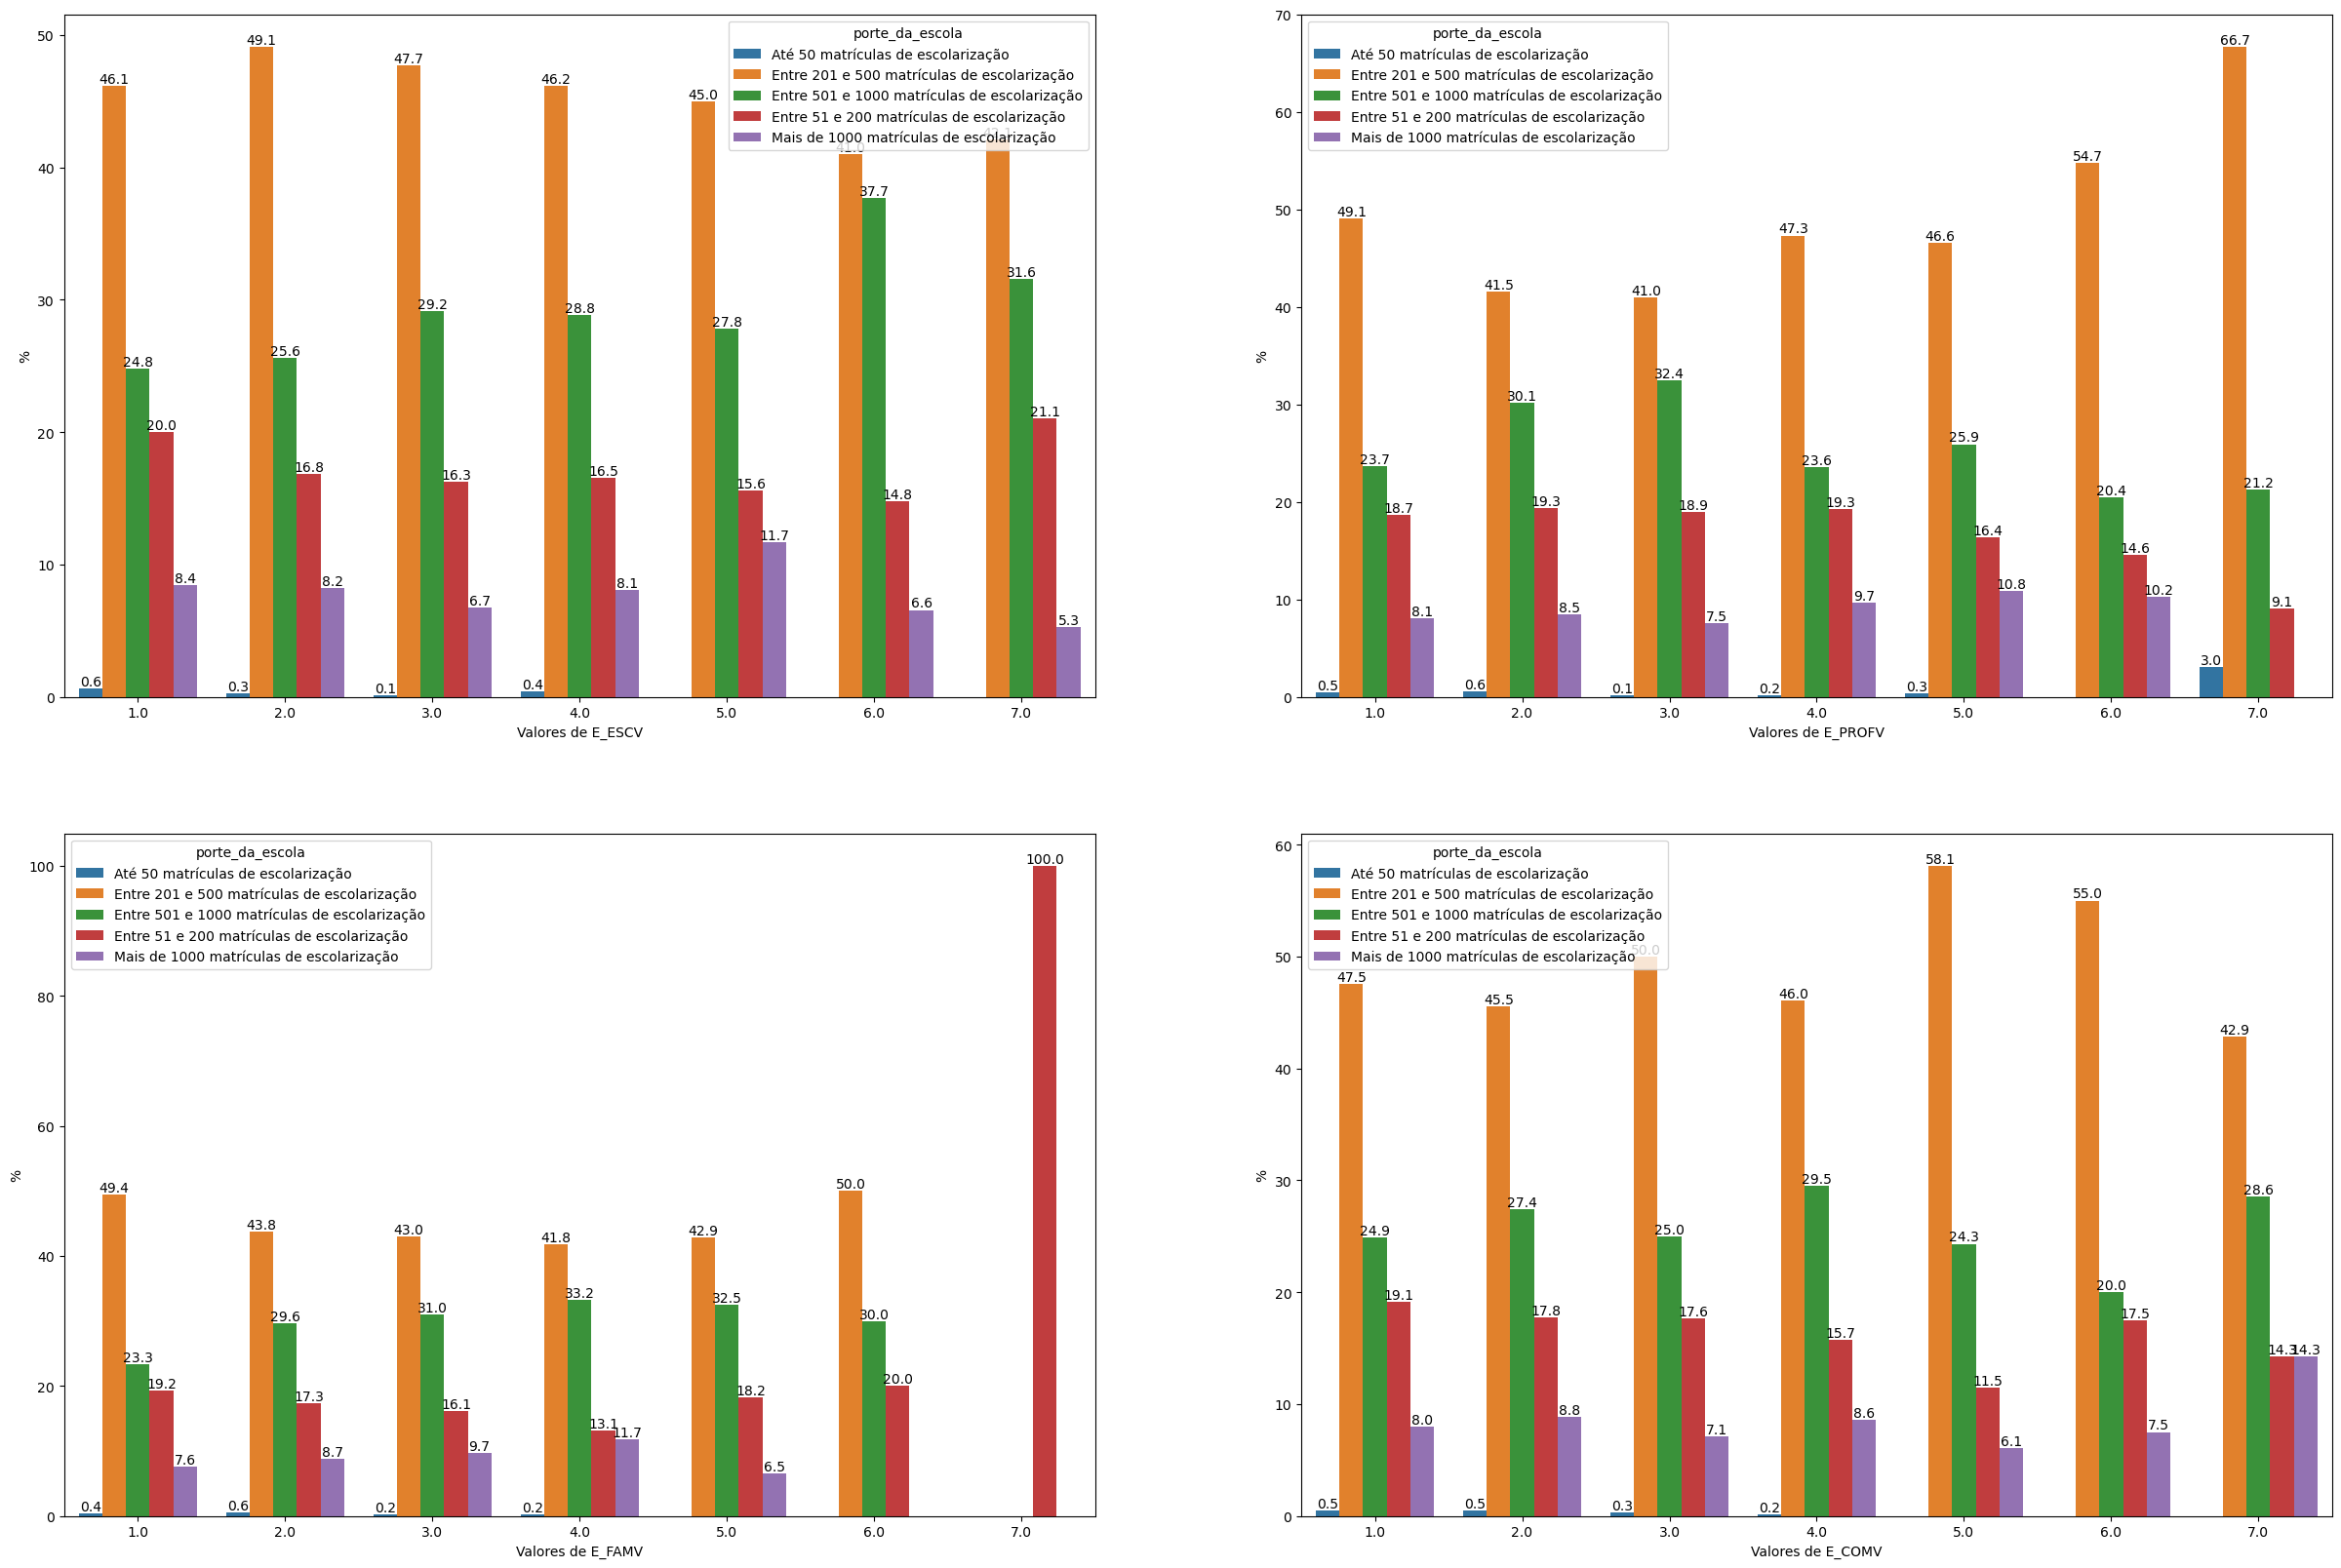
\includegraphics[width=1\textwidth]{Textuais/Imagens/Filé/porte_escola.png}
    \label{fig:porte_escola}
    \fonte{\me{2023}}
\end{figure}

 Na Figura \ref{fig:sexo} é possível notar que valores mais altos das dimensões E\_PROFV, E\_FAMV e E\_COMV apresentam uma porcentagem maior de estudantes homens do que mulheres, o que foi observado como sendo uma diferença significativa pelo p-valor. Essa diferença é especialmente grande para a dimensão E\_FAMV, onde 100\% dos alunos que obtiveram o valor 7.0 eram do sexo masculino.


\begin{figure}[ht!]
    \centering
    \caption{Correlação entre dimensões e sexo}
    \includegraphics[width=1\textwidth]{Textuais/Imagens/Filé/sexo.png}
    \label{fig:sexo}
    \fonte{\me{2023}}
\end{figure}

% \begin{figure}[ht!]
%     \centering
%     \includegraphics[width=1\textwidth]{Textuais/Imagens/Filé/uf.png}
%     \caption{Correlação entre dimensões e Unidade Federativa}
%     \label{fig:uf-dim}
% \end{figure}

A relação entre as dimensões E\_PROFV, E\_FAMV e E\_COMV e a localização dos estudantes pode ser vista na Figura \ref{fig:localizacao_dimensao}. Nela, é notável a porcentagem maior de estudantes na região urbana que possuem a nota mais alta para as dimensões analisadas, se comparado com estudantes da região rural.

\begin{figure}[ht!]
    \centering
    \caption{Correlação entre dimensões e localização}
    \includegraphics[width=1\textwidth]{Textuais/Imagens/Filé/localizacao.png}
    \label{fig:localizacao_dimensao}
    \fonte{\me{2023}}
\end{figure}

A Figura \ref{fig:renda-dimensoes} apresenta a relação entre a renda familiar do estudante e os fatores E\_ESCV, E\_FAMV e E\_COMV. Nela, é possível perceber que para os fatores E\_ESCV e E\_COMV, não há nenhum estudante que obteve as notas 6 e 7 cuja renda familiar é superior a 7 salários mínimos. Para a dimensão E\_FAMV, o valor 7 foi respondido 100\% por estudantes cuja renda familiar é de até um salário mínimo. Ainda, um ponto de destaque é que a nota 6 teve um pico de estudantes cuja renda familiar é superior a 9 salários mínimos.


\begin{figure}[ht!]
    \centering
    \caption{Correlação entre dimensões e renda familiar}
    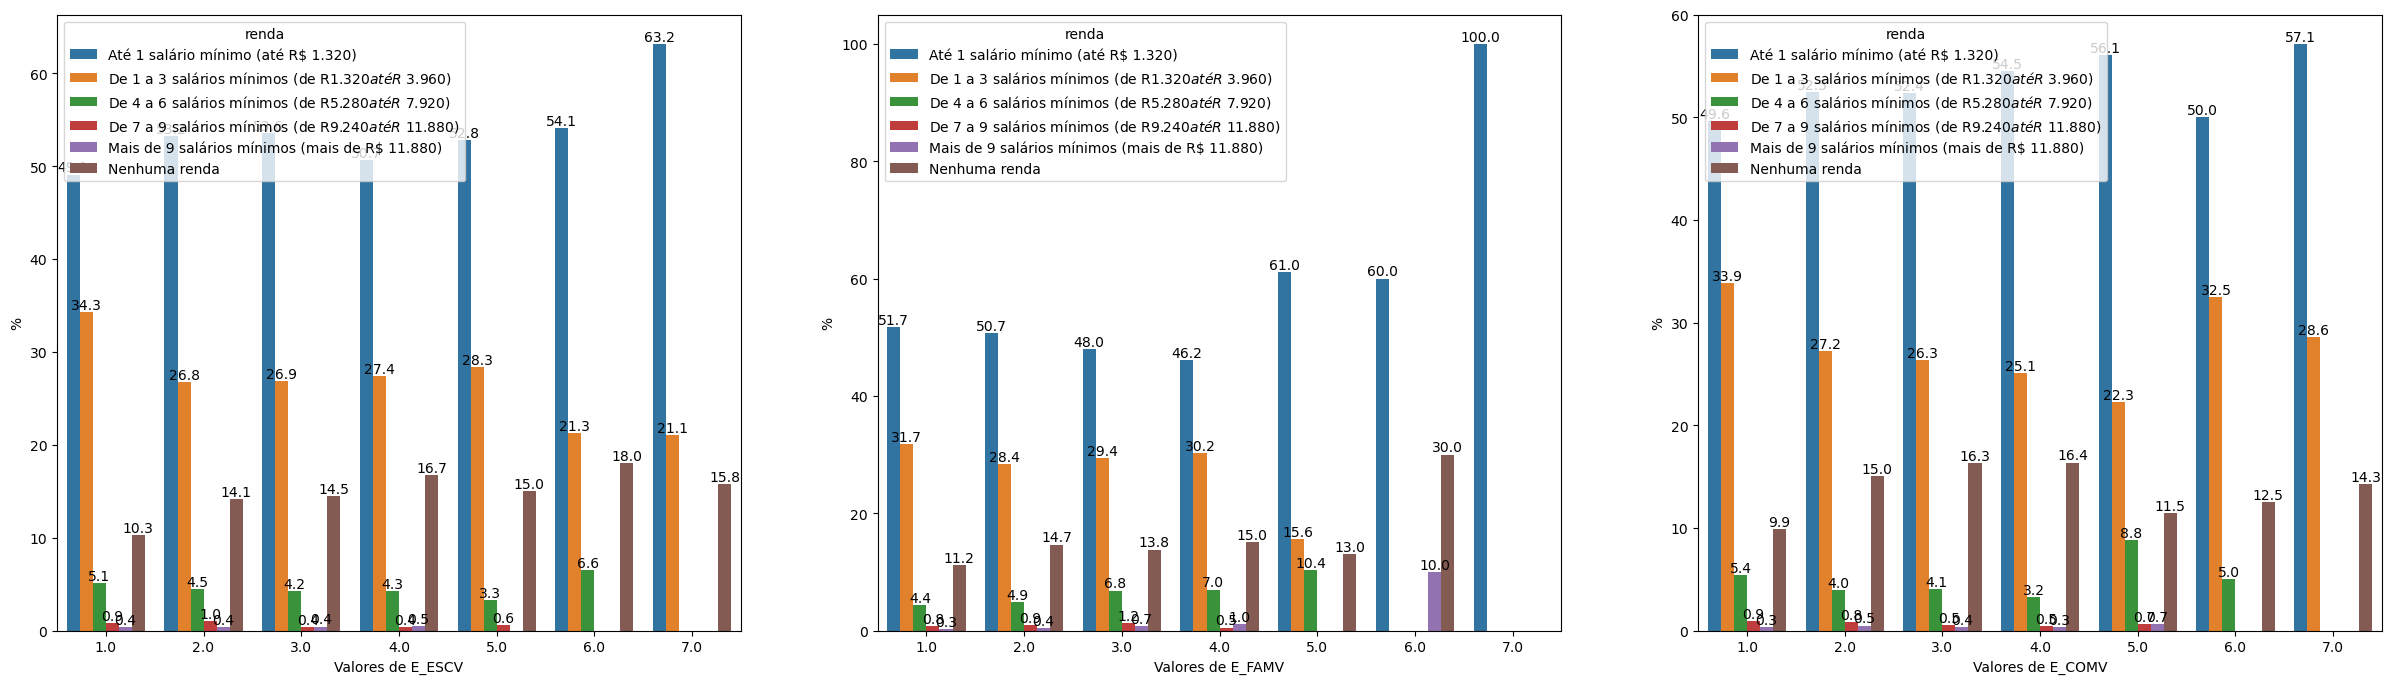
\includegraphics[width=1\textwidth]{Textuais/Imagens/Filé/renda.png}
    \label{fig:renda-dimensoes}
    \fonte{\me{2023}}
\end{figure}

Para a análise dos fatores, a Figura \ref{fig:fat-dependencia} apresenta a relação entre a dependência administrativa da escola do estudante com uma série de fatores distintos, cuja relação é significativa, conforme o p-valor observado. Com isso, alguns pontos de destaque desta relação são encontrados nos fatores E\_COM1V (Medidas Socioeducativas e Contextos de Violência), E\_EST3V (Reprovações e Distorção Idade – Série), onde a medida que a nota aumenta, a porcentagem de estudantes de escolas municipais aumenta e de escolas estaduais diminui. Outro ponto de destaque é o fator E\_FAM1V (Suporte Familiar), que para a nota 7, 100\% dos estudantes eram de escolas estaduais.


\begin{figure}[ht!]
    \centering
    \caption{Correlação entre fatores e dependência administrativa}
    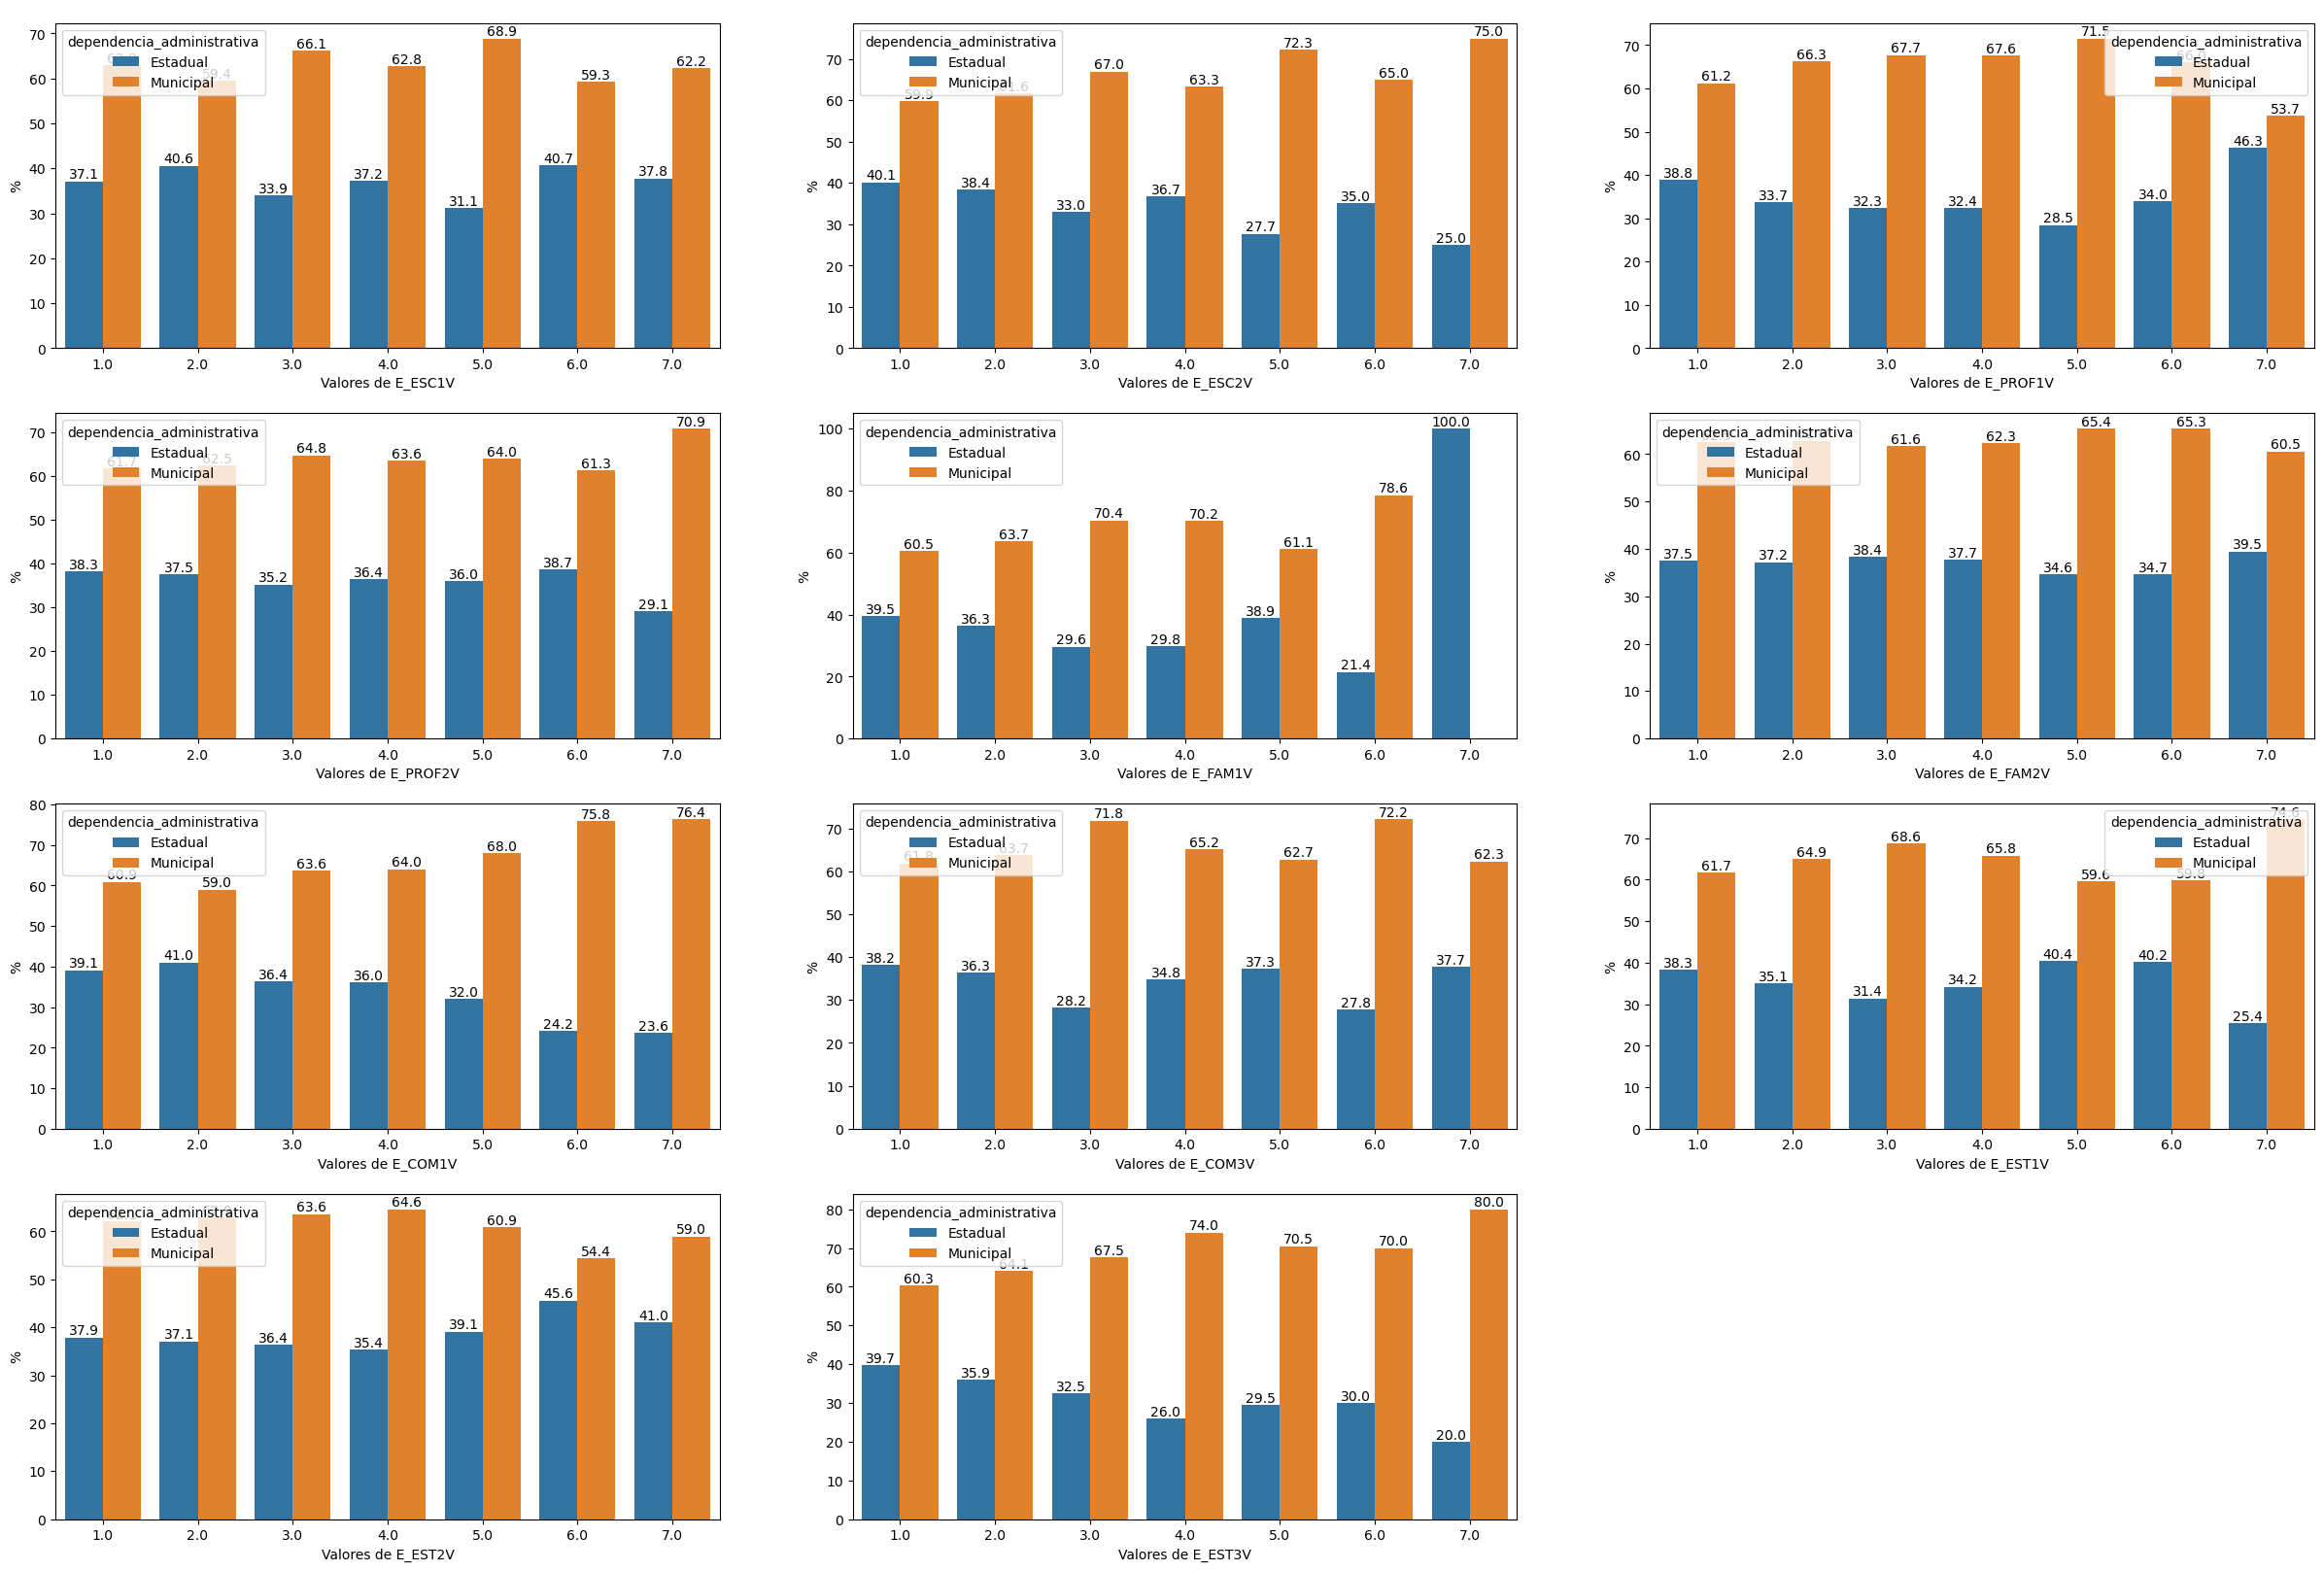
\includegraphics[width=1\textwidth]{Textuais/Imagens/Filé/dependencia_admin.png}
    \label{fig:fat-dependencia}
    \fonte{\me{2023}}
\end{figure}


Por fim, a Figura \ref{fig:sexo_fatores} apresenta a relação de fatores diversos com a variável sexo. Nela, os fatores E\_ESC2V (Condições Materiais do(a) Estudante) e E\_COM1V (Medidas Socioeducativas e Contextos de Violência) apresentam uma queda clara da porcentagem de estudantes do sexo feminino em detrimento do aumento dos estudantes do sexo masculino à medida que a nota para esses fatores aumenta. Outro ponto de interesse acontece no fator E\_FAM1V que para a nota 7, 100\% dos estudantes são do sexo masculino.


\begin{figure}[ht!]
    \centering
    \caption{Correlação entre fatores e sexo}
    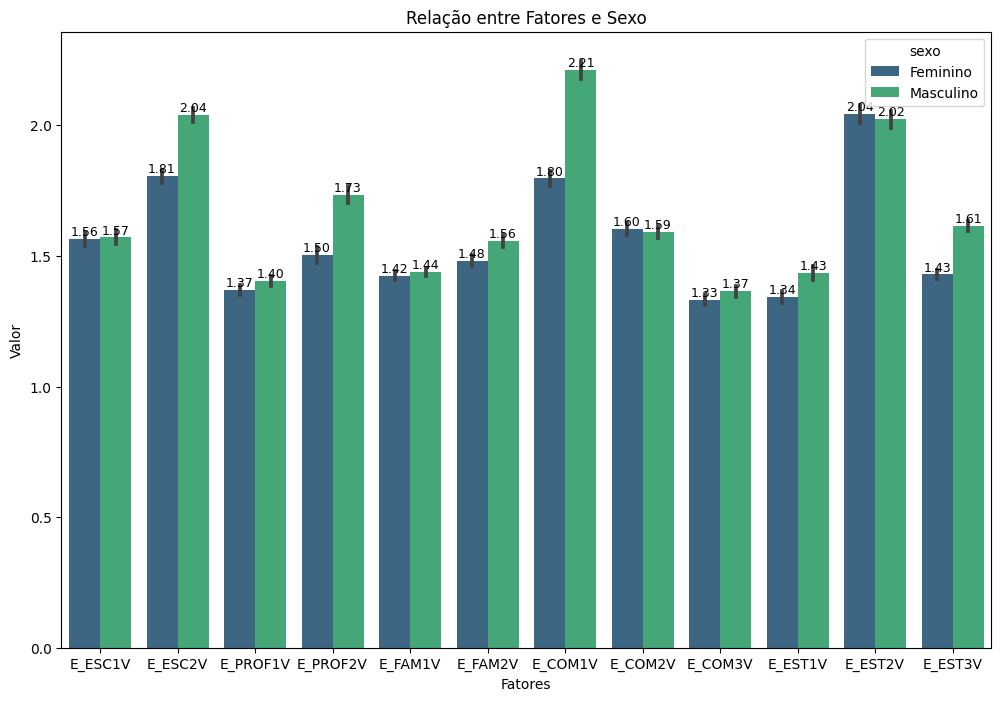
\includegraphics[width=1\textwidth]{Textuais/Imagens/Filé/sexo_fatores.png}
    \label{fig:sexo_fatores}
    \fonte{\me{2023}}
\end{figure}

No entanto, é possível notar que a distribuição de valores do número de estudantes de cada categoria é bastante desigual, com, por exemplo, uma porcentagem muito maior de estudantes do sexto, sétimo, oitavo e nono ano do que dos demais. Esse desbalanço, que ocorre em diversas variáveis sociodemográficas, pode ser um grande influenciador dos resultados obtidos para o p-valor.

Outra métrica analisada para identificar padrões de associação ou dependência entre as diferentes dimensões do conjunto de dados foi traçar uma análise de correlação entre as variáveis das dimensões e entre as variáveis dos fatores para analisar qual delas poderia ter mais influência uma sobre as outras. Essas matrizes de correlações são representadas pelas Figuras \ref{fig:matriz-correlacao-dimensoes} e \ref{fig:matriz-correlacao-fatores}. Nelas, é possível verificar que quando os números estão mais próximos de 1.0 significa que há uma maior correlação positiva entre as variáveis, e quando estão próximos de -1.0, há uma maior correlação negativa, com valores próximos a zero não possuindo muita significância. É importante lembrar que enquanto duas variáveis estão correlacionadas uma à outra, isso não significa que uma implica na causalidade da outra.

Tendo isso em mente, é notável na Figura \ref{fig:matriz-correlacao-dimensoes} a correlação positiva mediana que há entre as dimensões E\_PROFV e E\_COMV, com 0.41, atingindo o maior número dentre as dimensões. Ou seja, isso significa que há uma tendência de quando os valores de E\_COMV forem mais altos, há maior probabilidade de E\_PROFV também serem, indicando que há uma interligação entre esses dois fatores dentro do questionário. 

\begin{figure}[ht!]
    \centering
    \caption{Correlação entre dimensões}
    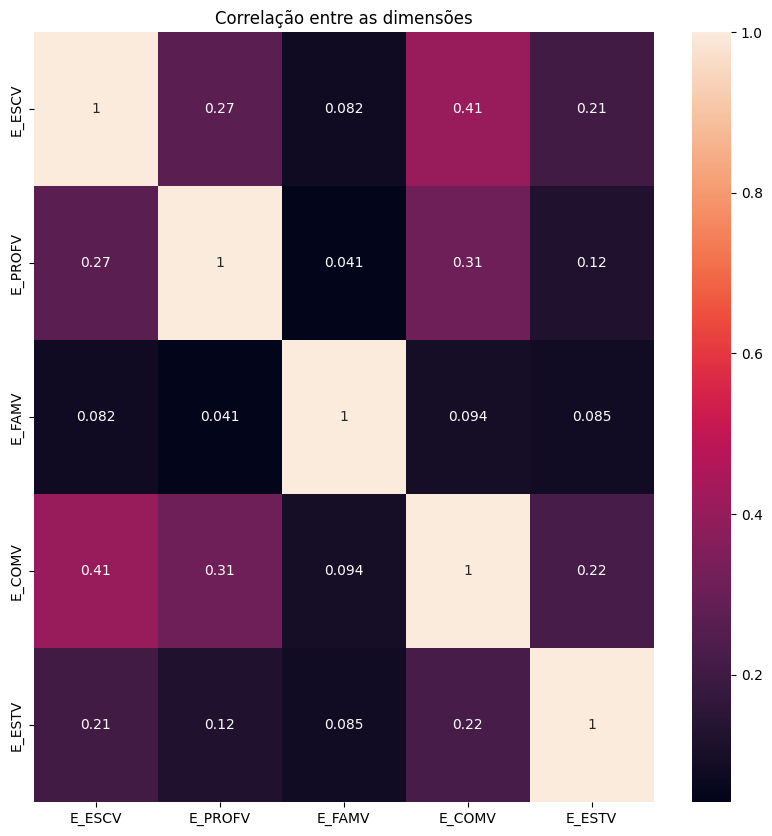
\includegraphics[width=0.7\textwidth]{Textuais/Imagens/Filé/correlacao_dimensoes.png}
    \label{fig:matriz-correlacao-dimensoes}
    \fonte{\me{2023}}
\end{figure}

Já na Figura \ref{fig:matriz-correlacao-fatores}, percebe-se que o fator E\_FAM1V (Suporte Familiar) é o que possui correlação negativa com a maioria todos os outros fatores, exceto com E\_EST3V (Reprovações e Distorção idade-série), o que indica que é uma variável significativa mesmo que inversamente proporcional às outras. É importante ressaltar que o fator E\_EST3V também possui em sua maioria correlação negativa com os outros fatores, mas são valores mais próximos de zero que a variável anterior, indicando que possui menos significância estatística correlacional. Nota-se também que os fatores E\_FAM2V (Gravidez/parentalidade/atividades de cuidado) e E\_COM2V (Acessibilidade e frequência escolar) são os que possuem maior correlação positiva com a maioria dos outros fatores, com seus valores positivos ficando entre 0.13 a 0.38 e 0.11 a 0.33, respectivamente.

\begin{figure}[ht!]
    \centering
    \caption{Correlação entre fatores}
    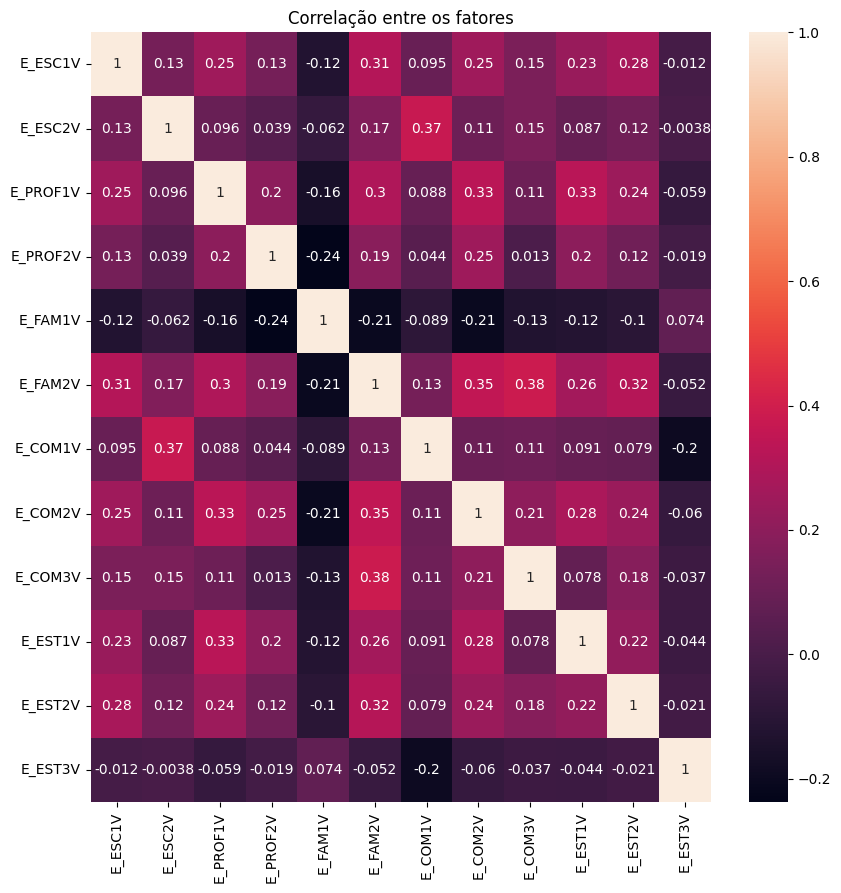
\includegraphics[width=0.8\textwidth]{Textuais/Imagens/Filé/correlacao_fatores.png}
    \label{fig:matriz-correlacao-fatores}
    \fonte{\me{2023}}
\end{figure}

Após as análises estatísticas feitas, o próximo passo da pesquisa são as análises classificatórias com o auxílio de \textit{machine learning}, a ser realizado no próximo capítulo.

%%%%%%%%%%%%%%%%%%%%%%%%%%%%%%%%%%%

% Por fim, foi decidido estudar o relacionamento das médias das dimensões e fatores em comparação com variáveis estatísticas exclusivas dos estudantes, resultando nos gráficos das Figuras \ref{fig:dimensoes-etnia}, \ref{fig:fatores-etnia}, \ref{fig:dimensoes-sexo}, \ref{fig:fatores-sexo}, \ref{fig:dimensoes-anoensino}, \ref{fig:fatores-anoensino}, \ref{fig:dimensoes-anoensino-radar} e \ref{fig:fatores-anoensino-radar}.

% \begin{figure}[ht!]
%     \centering
%     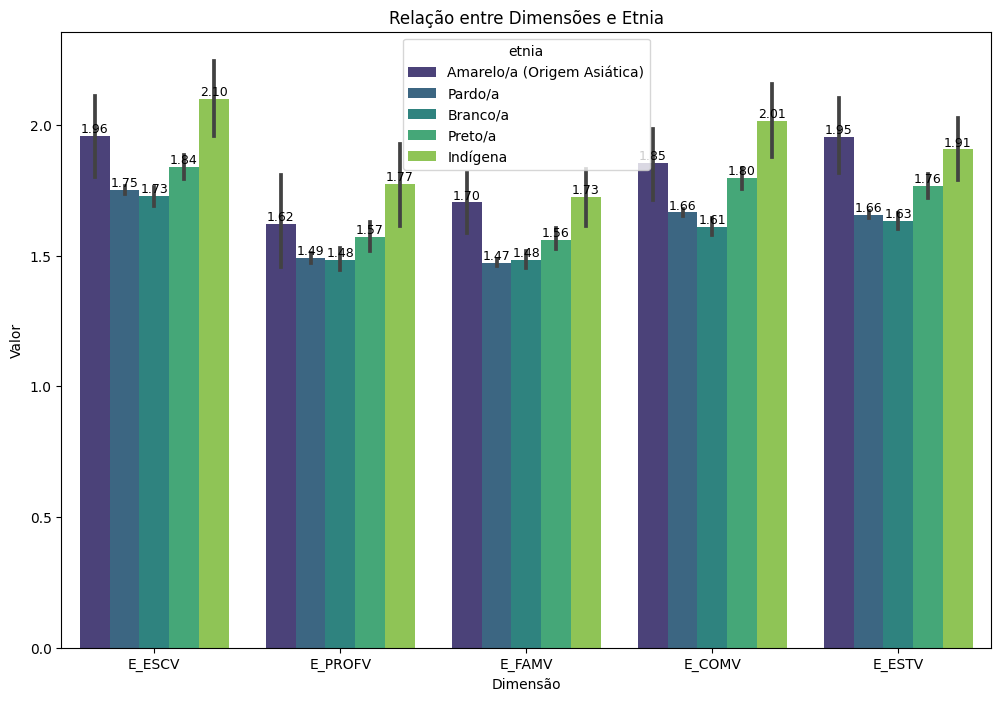
\includegraphics[width=0.8\textwidth]{Textuais/Imagens/Filé/output.png}
%     \caption{Relação entre dimensões e etnia dos estudantes}
%     \label{fig:dimensoes-etnia}
% \end{figure}

% \begin{figure}[ht!]
%     \centering
%     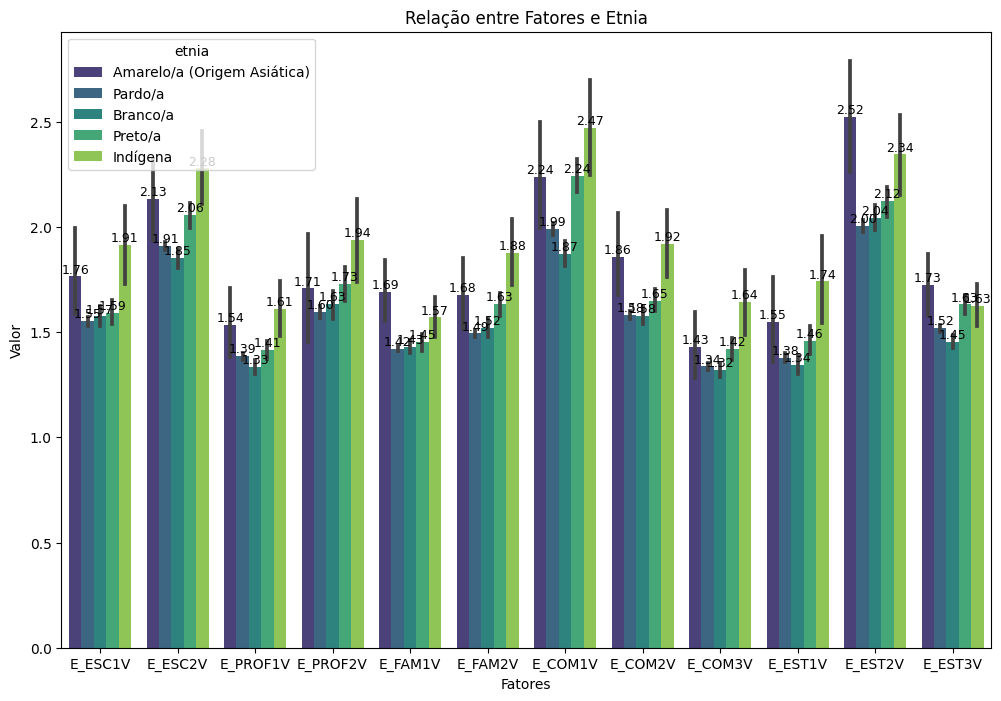
\includegraphics[width=0.8\textwidth]{Textuais/Imagens/Filé/output1.png}
%     \caption{Relação entre fatores e etnia dos estudantes}
%     \label{fig:fatores-etnia}
% \end{figure}

% \begin{figure}[ht!]
%     \centering
%     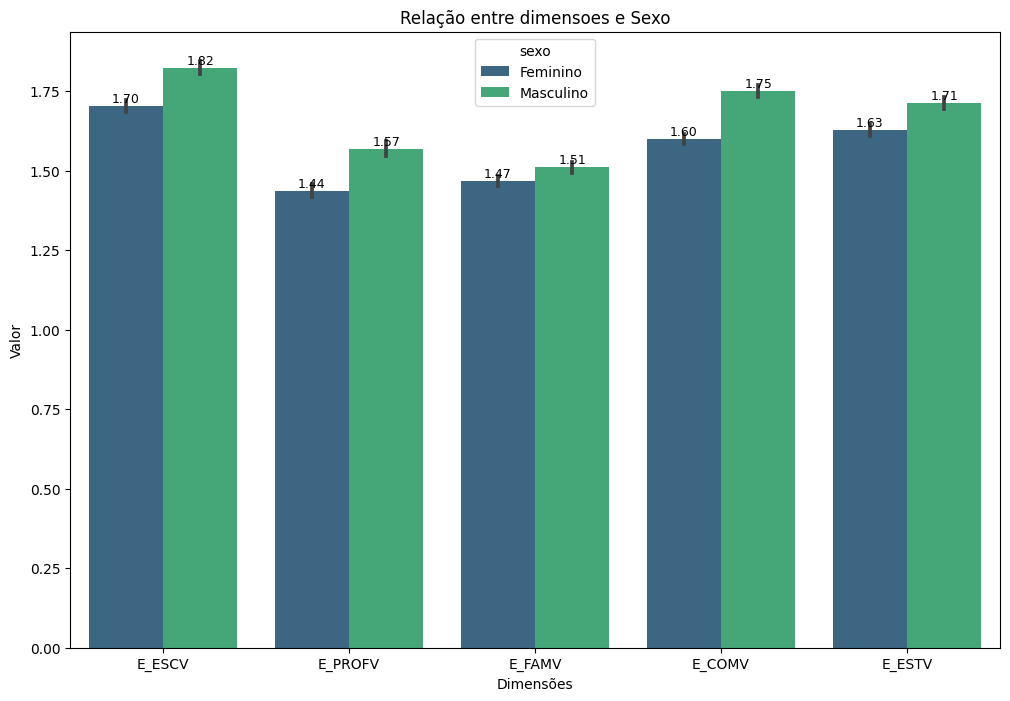
\includegraphics[width=0.8\textwidth]{Textuais/Imagens/Filé/output2.png}
%     \caption{Relação entre dimensões e sexo dos estudantes}
%     \label{fig:dimensoes-sexo}
% \end{figure}

% \begin{figure}[ht!]
%     \centering
%     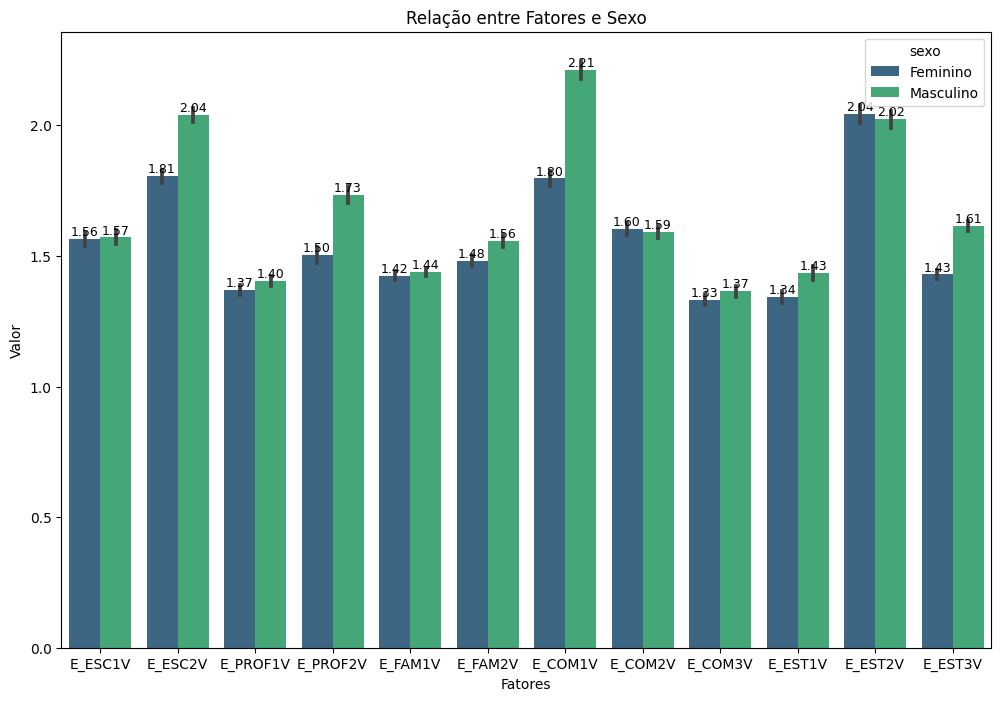
\includegraphics[width=0.8\textwidth]{Textuais/Imagens/Filé/output3.png}
%     \caption{Relação entre fatores e sexo dos estudantes}
%     \label{fig:fatores-sexo}
% \end{figure}

% \begin{figure}[ht!]
%     \centering
%     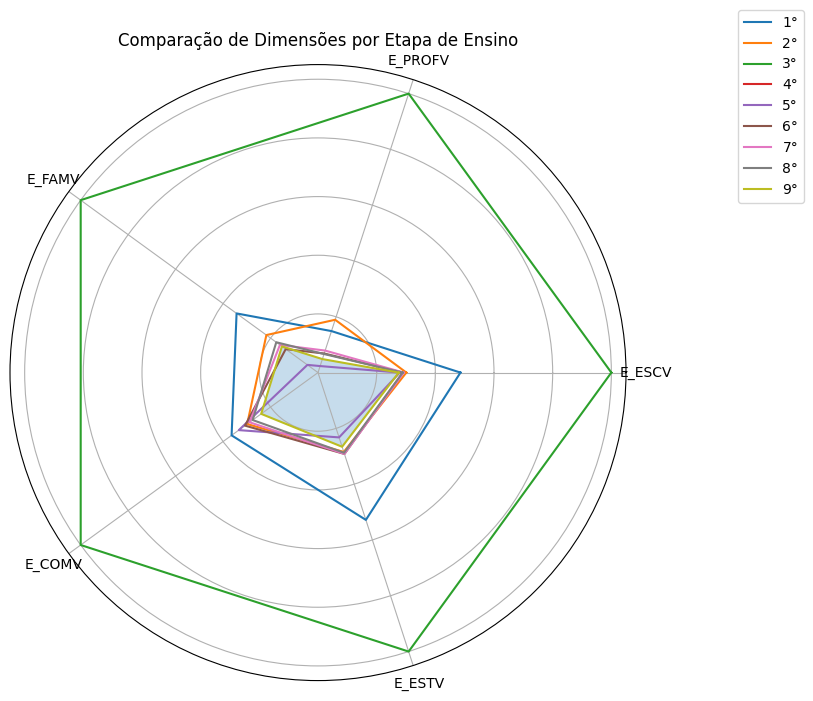
\includegraphics[width=0.8\textwidth]{Textuais/Imagens/Filé/radar_dimensoes.png}
%     \caption{Relação entre dimensões e ano de ensino dos estudantes}
%     \label{fig:dimensoes-anoensino}
% \end{figure}

% \begin{figure}[ht!]
%     \centering
%     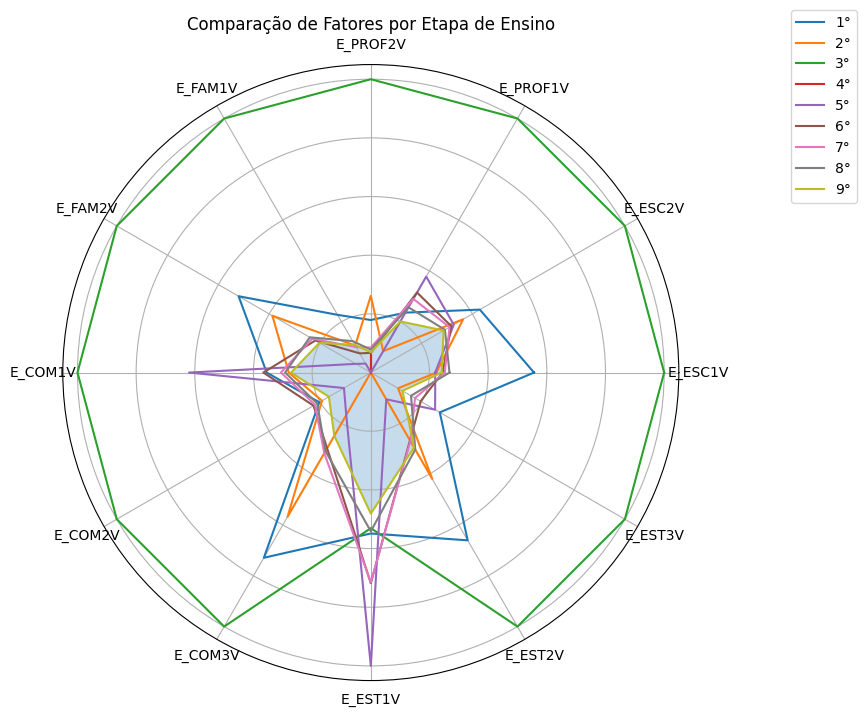
\includegraphics[width=0.8\textwidth]{Textuais/Imagens/Filé/radar_fatores.png}
%     \caption{Relação entre fatores e ano de ensino dos estudantes}
%     \label{fig:fatores-anoensino}
% \end{figure}

% \begin{figure}[ht!]
%     \centering
%     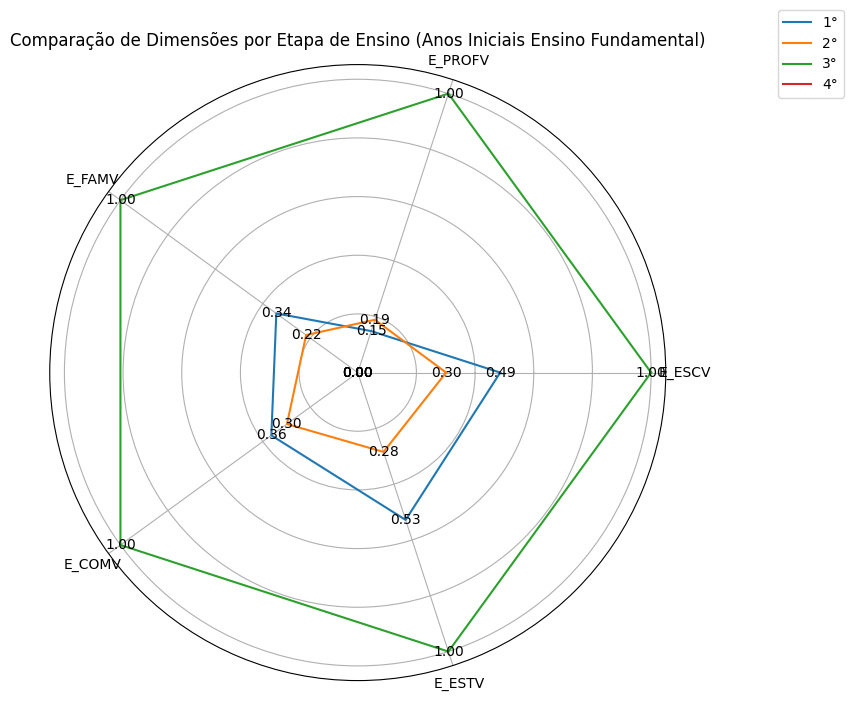
\includegraphics[width=0.4\textwidth]{Textuais/Imagens/Filé/radar_dimensoes_iniciais.png}
%     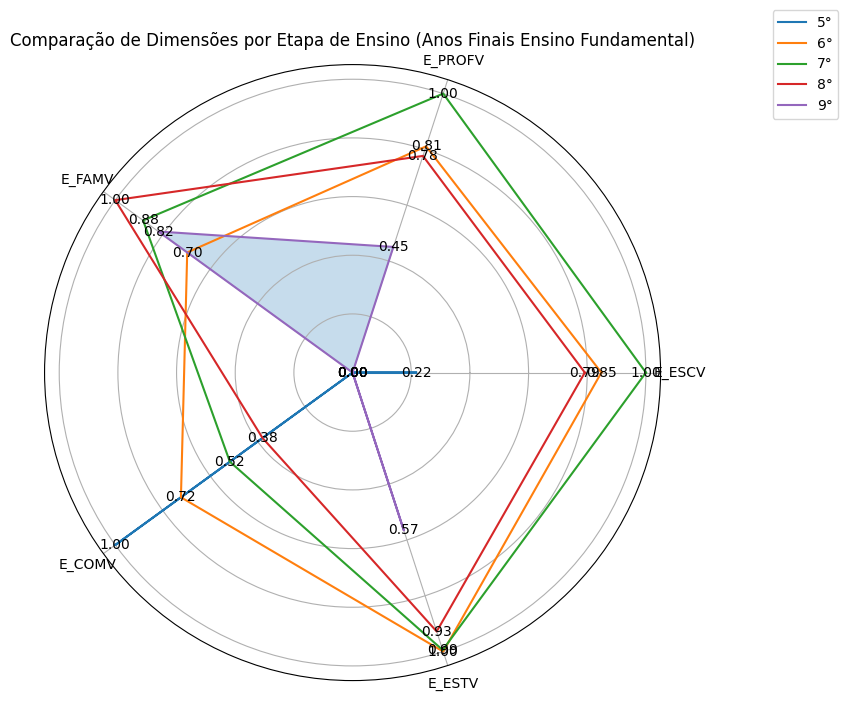
\includegraphics[width=0.4\textwidth]{Textuais/Imagens/Filé/radar_dimensoes_finais.png}
%     \caption{Relação entre dimensões e ano de ensino dos estudantes}
%     \label{fig:dimensoes-anoensino-radar}
% \end{figure}


% \begin{figure}[ht!]
%     \centering
%     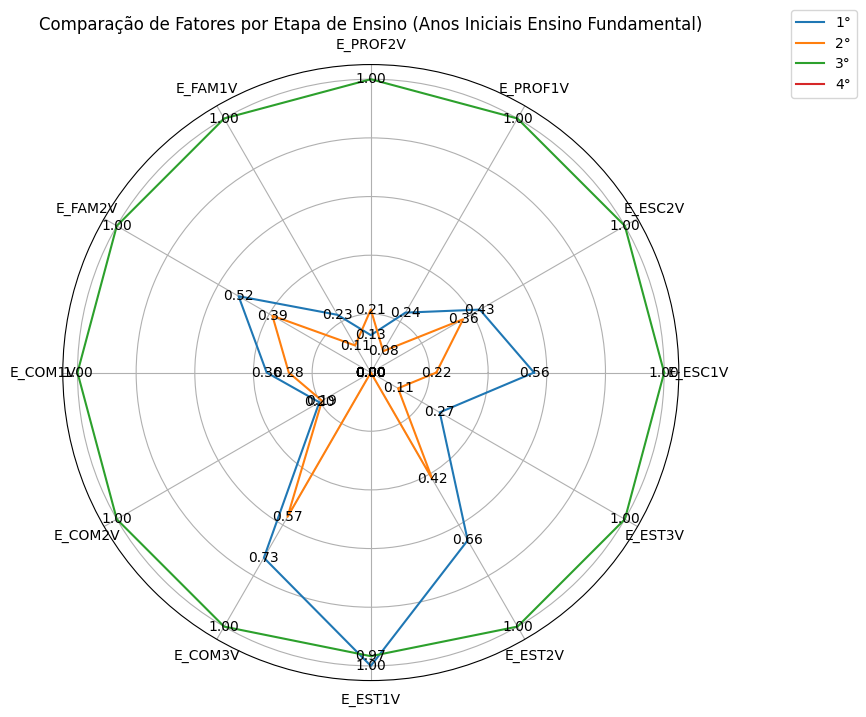
\includegraphics[width=0.4\textwidth]{Textuais/Imagens/Filé/radar_fatores_iniciais.png}
%     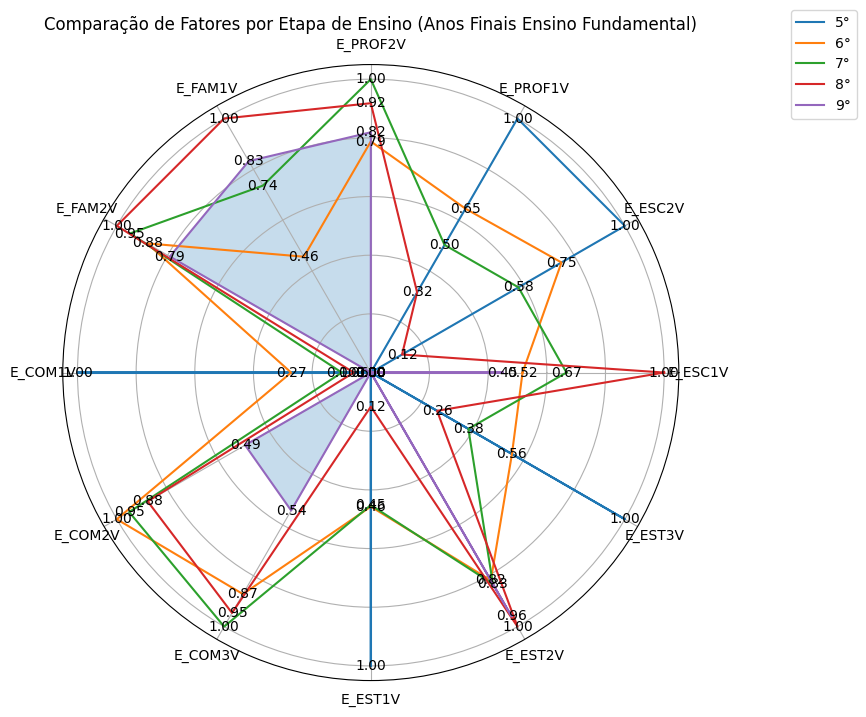
\includegraphics[width=0.4\textwidth]{Textuais/Imagens/Filé/radar_fatores_finais.png}
%     \caption{Relação entre fatores e ano de ensino dos estudantes}
%     \label{fig:fatores-anoensino-radar}
% \end{figure}
% \chapter{Análises classificatórias}

Por mais que houve o estudo realizado na área de reconhecimento de padrões em \textit{machine learning}, após o recebimento da base foi notado que a base era composta principalmente por instâncias rotuladas, ou seja, as classes eram conhecidas e possíveis de categorização. Além disso, já que a base não está afirmando quais alunos irão evadir, apenas mostrando respostas possíveis de estudantes a um questionário, é mais interessante de um ponto de vista científico afirmar quais variáveis possuem o maior peso de predição de influência dentro do questionário. Sendo assim, foi concluído que a melhor estratégia adotada para o trabalho foi não a de reconhecer padrões, mas sim a de aplicação de técnicas de classificação em \textit{machine learning}, sem alteração nos algoritmos que serão utilizados para análise.

Para fazer a aplicação dos métodos na base, alguns cuidados foram necessários para que os modelos não tivessem problemas em suas análises e treinamento.

O primeiro passo foi retratar os dados de valores reais para valores inteiros. Isso acontece porque, como estamos lidando com um problema de classificação, cada fração seria considerada uma classe diferente. Ou seja, valores como ``3.0'' e ``3.333333'' são considerados duas classes diferentes. Para que fosse melhor identificado a classe que um aluno poderia estar, foi arredondado todos os valores de ponto flutuante, arredondando os valores para cima caso tivessem sua primeira casa após a vírgula 5 em diante (ou seja, valores como 2.5 e 2.6666667 foram considerados 3.0, enquanto 2.3333333 foi considerado 2).

Além disso, como é possível verificar pelos histogramas das Figuras \ref{fig:histograma-dimensoes} e \ref{fig:histograma-fatores}, havia um severo desbalanceamento da base em todas as variáveis, tanto nas categorias de dimensão quanto na de fatores. Para cada variável, havia grande número de respostas distribuídas entre os valores 1 a 3, e poucas respostas classificadas entre 5 a 7. Isso significa que foi necessário realizar um balanceamento da base, evitando um desempenho enviesado em relação a uma das classes. Apenas durante o treinamento dos modelos para cada dimensão e cada fator, foi escolhida a classe com o maior número de respostas, e todas as outras classes foram redistribuídas.

\begin{figure}[htp!]
    \centering
    \caption{Histograma Dimensões}
    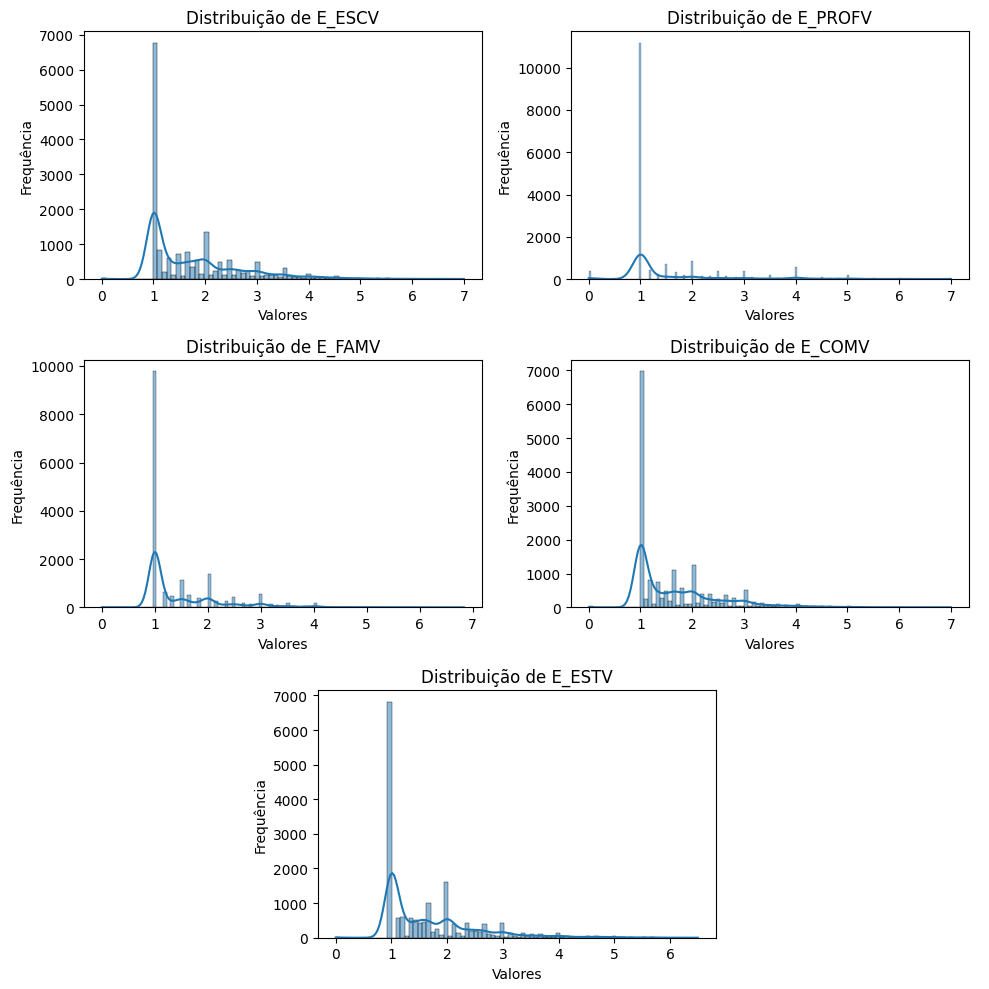
\includegraphics[width=0.75\textwidth]{Textuais/Imagens/Gráficos/histograma_dimensoes.png}
    \label{fig:histograma-dimensoes}
    \fonte{\me{2023}}
\end{figure}

\begin{figure}[htp!]
    \centering
    \caption{Histograma Fatores}
    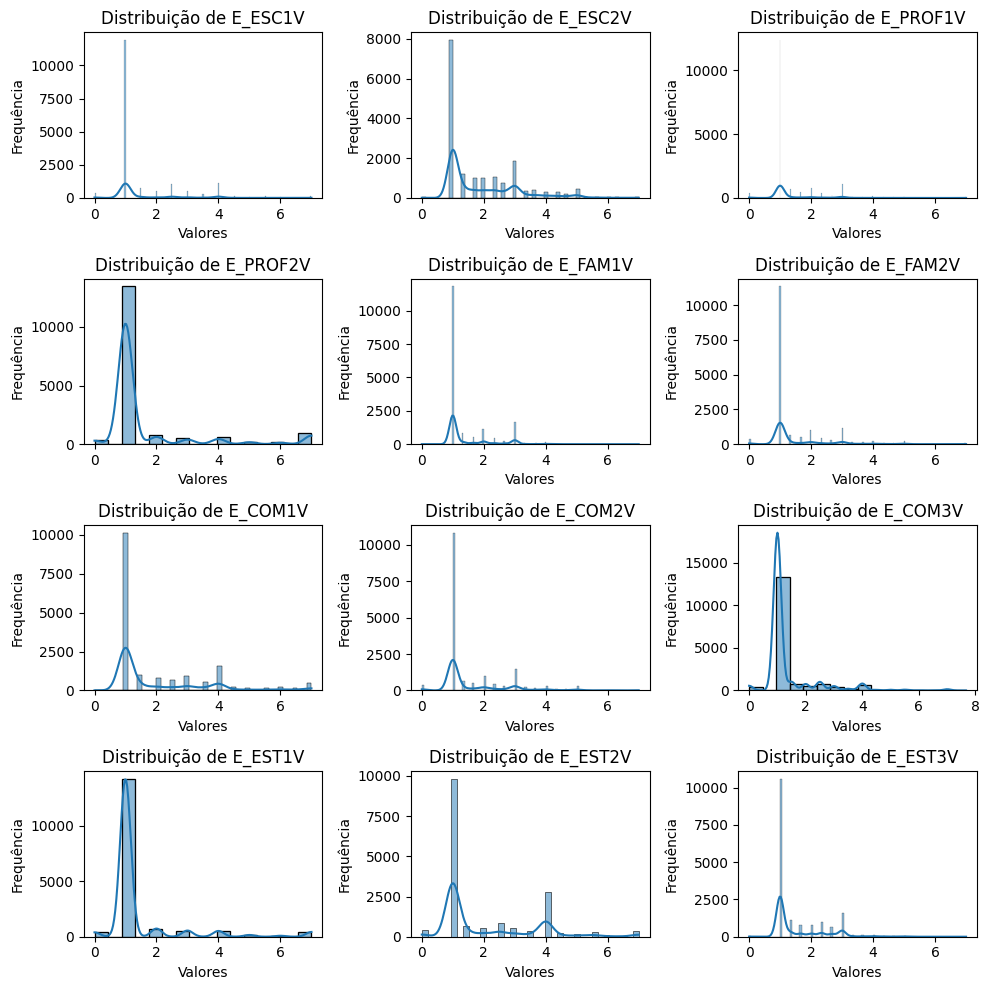
\includegraphics[width=0.8\textwidth]{Textuais/Imagens/Gráficos/histograma_fatores.png}
    \label{fig:histograma-fatores}
    \fonte{\me{2023}}
\end{figure}

Também é importante informar que durante os testes, não foram divididos de forma fixa conjunto de dados para treinamento, teste e validação, e eles eram distintos entre si. A cada iteração do código, 20\% da base era aleatoriamente escolhida para tratar como teste, querendo evitar desempenhos superestimados, pois caso não fosse tomado esse cuidado, os modelos já teriam visto os dados de teste durante o treinamento.

É relevante informar que para além das métricas escolhidas para avaliação dos modelos como consta na seção \ref{subsec:tecnicas}, também foram feitas a visualização das matrizes de confusão para melhor compreensão acerca da \textit{performance} dos modelos escolhidos. Todas as matrizes de confusão encontram-se nos Apêndices \ref{ap1}, \ref{ap2}, \ref{ap3}, \ref{ap4} e \ref{ap5} deste trabalho.

Por fim, os algoritmos foram todos treinados utilizando a linguagem de programação Python 3.10, com o auxílio da biblioteca \textit{sklearn}. Foram utilizados os seguintes modelos para treinamento dentro da biblioteca: DecisionTreeClassifier, RandomForestClassifier, AdaBoostClassifier, CategoricalNB e KNeighborsClassifier. Os algoritmos foram testados em uma máquina que continha as seguintes especificações: \textit{OS: Windows 10 19045.3448 x86\_64;
RAM: 24 GB;
CPU: Intel Core(TM) i5-7400 CPU @ 3.00GHz;
GPU: RTX 3060 12GB}.

A seguir, são apresentados os resultados dos algoritmos escolhidos após sua aplicação no banco de dados, destacando as variáveis que obtiveram os melhores resultados classificatórios.

\section{Decision Tree}

A análise das Tabelas \ref{tab:dimensoes_decision_tree_classifier} e \ref{tab:fatores_decision_tree} revela algumas informações importantes sobre o desempenho do modelo de Decision Tree nas diferentes dimensões testadas. Inicialmente, é perceptível que os valores de acurácia para todas as variáveis são relativamente altos, variando de aproximadamente 74\% a 99\%, indicando, em geral, uma boa capacidade do modelo em prever corretamente as classes.

\begin{table}[ht]
    \centering
    \caption{Dimensões sendo testadas no modelo de Decision Tree}
    \resizebox{0.8\textwidth}{!}{%
    \begin{tabular}{|c|c|c|c|c|}
    \hline
    \textbf{Variável} & \textbf{Acurácia} & \textbf{Precisão} & \textbf{Recall Score} & \textbf{F1 Score} \\ \hline
    \textbf{E\_ESCV}  & 0.751673360 & 0.739981653 & 0.751673360 & 0.741630082 \\ \hline
    \textbf{E\_PROFV} & 0.783035930 & 0.786358820 & 0.783035930 & 0.777129550 \\ \hline
    \textbf{E\_FAMV}  & 0.830982219 & 0.831129806 & 0.830982219 & 0.827472004 \\ \hline
    \textbf{E\_COMV}  & 0.774183466 & 0.769368781 & 0.774183466 & 0.767111565 \\ \hline
    \textbf{E\_ESTV}  & 0.741793911 & 0.732561420 & 0.741793911 & 0.732551048 \\ \hline
    \end{tabular}%
    }
    \label{tab:dimensoes_decision_tree_classifier}
    \fonte{\me{2023}}
\end{table}

\begin{table}[ht]
    \centering
    \caption{Fatores sendo testados no modelo Decision Tree}
    \resizebox{0.8\textwidth}{!}{%
    \begin{tabular}{|c|c|c|c|c|}
        \hline
        \textbf{Variável} & \textbf{Acurácia} & \textbf{Precisão} & \textbf{Recall Score} & \textbf{F1 Score} \\ \hline
        \textbf{E\_ESC1V}  & 0.973298932 & 0.974228894 & 0.973298932 & 0.972954891 \\ \hline
        \textbf{E\_ESC2V}  & 0.957975316 & 0.958817154 & 0.957975316 & 0.957990201 \\ \hline
        \textbf{E\_PROF1V} & 0.985004378 & 0.985474842 & 0.985004378 & 0.984873283 \\ \hline
        \textbf{E\_PROF2V} & 0.995594947 & 0.995617592 & 0.995594947 & 0.995594299 \\ \hline
        \textbf{E\_FAM1V}  & 0.981763607 & 0.982526522 & 0.981763607 & 0.981566092 \\ \hline
        \textbf{E\_FAM2V}  & 0.988539873 & 0.988990114 & 0.988539873 & 0.988512460 \\ \hline
        \textbf{E\_COM1V}  & 0.957073377 & 0.958085738 & 0.957073377 & 0.956205580 \\ \hline
        \textbf{E\_COM2V}  & 0.977282629 & 0.978631022 & 0.977282629 & 0.976942412 \\ \hline
        \textbf{E\_COM3V}  & 0.988506982 & 0.989023192 & 0.988506982 & 0.988421136 \\ \hline
        \textbf{E\_EST1V}  & 0.987947572 & 0.988248921 & 0.987947572 & 0.987787534 \\ \hline
        \textbf{E\_EST2V}  & 0.973289665 & 0.974189465 & 0.973289665 & 0.973112790 \\ \hline
        \textbf{E\_EST3V}  & 0.986756179 & 0.987237780 & 0.986756179 & 0.986687563 \\ \hline
    \end{tabular}%
    }
    \fonte{\me{2023}}
    \label{tab:fatores_decision_tree}
\end{table}

Ao observar as métricas de precisão, recall e F1 Score, nota-se uma consistência nos resultados para cada variável. No geral, as métricas de precisão e recall são bastante equilibradas, indicando que o modelo consegue manter um bom equilíbrio entre a identificação correta das instâncias positivas e a minimização de falsos positivos.

Entretanto, ao analisar mais profundamente, percebe-se que o fator \textbf{E\_ESC1V} (Condições Materiais da Escola) se destaca com valores extremamente altos em todas as métricas, com acurácia, precisão, recall e F1 Score superiores a 97\%. Isso sugere que o modelo possui um desempenho excepcional ao lidar com essa variável específica, indicando possivelmente uma característica única ou padrão distinto nessa dimensão.

Por outro lado, a dimensão \textbf{E\_ESTV} (Estudante-Estudante) apresenta valores ligeiramente inferiores em comparação com as outras variáveis, especialmente em termos de acurácia e F1 Score. Isso pode indicar que essa dimensão é mais desafiadora para o modelo, seja devido à complexidade dos padrões presentes nos dados ou a uma menor representatividade das características distintivas.

Comparando as métricas, nota-se que, considerando a acurácia geral, o fator \textbf{E\_ESC1V} se destaca. No entanto, as dimensões \textbf{E\_PROFV} (Estudante-Profissionais da
Escola)  ou \textbf{E\_FAMV} (Estudante-Família) também se destacam por possuírem equilíbrio entre precisão e recall. Por outro lado, a pior variável para predição, ou seja, que apresentou os piores valores nas métricas, é a dimensão \textbf{E\_ESTV} (Estudante-Estudante).


%%%%%%%%%%%%%%%%%%%%%%%%%%%

\section{Random Forest}

Ao analisar as Tabelas \ref{tab:dimensoes_random_forest_classifier} e \ref{tab:fatores_random_forest_classifier}, algumas observações são notáveis. Na tabela referente às dimensões, as variáveis \textbf{E\_ESCV} (Estudante-Escola) \textbf{E\_FAMV} (Estudante-Família) se destacam com os maiores valores em todas as métricas, indicando um bom desempenho global do modelo nas duas dimensões.

\begin{table}[ht]
    \centering
    \caption{Dimensões sendo testadas no modelo Random Forest}
    \resizebox{0.8\textwidth}{!}{%
    \begin{tabular}{|c|c|c|c|c|}
    \hline
    \textbf{Variável} & \textbf{Acurácia} & \textbf{Precisão} & \textbf{Recall Score} & \textbf{F1 Score} \\ \hline
    \textbf{E\_ESCV}  & 0.848055295	& 0.842921845 & 0.848055295 & 0.843924479 \\ \hline
    \textbf{E\_PROFV} & 0.786592718 & 0.790278008 & 0.786592718 & 0.781311994 \\ \hline
    \textbf{E\_FAMV}  & 0.833147431 & 0.831530566 & 0.833147431 & 0.829228533 \\ \hline
    \textbf{E\_COMV}  & 0.778324738 & 0.770605436 & 0.778324738 & 0.771282145 \\ \hline
    \textbf{E\_ESTV}  & 0.744445460 & 0.734167526 & 0.744445460 & 0.735079615 \\ \hline
    \end{tabular}%
    }
    \fonte{\me{2023}}
    \label{tab:dimensoes_random_forest_classifier}
\end{table}

\begin{table}[ht]
    \centering
    \caption{Fatores sendo testados no modelo Random Forest}
    \resizebox{0.8\textwidth}{!}{%
    \begin{tabular}{|c|c|c|c|c|}
        \hline
        \textbf{Variável} & \textbf{Acurácia} & \textbf{Precisão} & \textbf{Recall Score} & \textbf{F1 Score} \\ \hline
        \textbf{E\_ESC1V}  & 0.979659186 & 0.980308426 & 0.979659186 & 0.979535759 \\ \hline
        \textbf{E\_ESC2V}  & 0.964458678 & 0.964734405 & 0.964458678 & 0.964430198 \\ \hline
        \textbf{E\_PROF1V} & 0.988178634 & 0.988461239 & 0.988178634 & 0.988120343 \\ \hline
        \textbf{E\_PROF2V} & 0.996337968 & 0.996351606 & 0.996337968 & 0.996338277 \\ \hline
        \textbf{E\_FAM1V}  & 0.982499858 & 0.983288480 & 0.982499858 & 0.982314134 \\ \hline
        \textbf{E\_FAM2V}  & 0.990855650 & 0.991095707 & 0.990855650 & 0.990836153 \\ \hline
        \textbf{E\_COM1V}  & 0.968210333 & 0.968547724 & 0.968210333 & 0.967829172 \\ \hline
        \textbf{E\_COM2V}  & 0.982635215 & 0.983218686 & 0.982635215 & 0.982435642 \\ \hline
        \textbf{E\_COM3V}  & 0.992910849 & 0.993159647 & 0.992910849 & 0.992893850 \\ \hline
        \textbf{E\_EST1V}  & 0.996836238 & 0.996854884 & 0.996836238 & 0.996829868 \\ \hline
        \textbf{E\_EST2V}  & 0.981295488 & 0.981635502 & 0.981295488 & 0.981176100 \\ \hline
        \textbf{E\_EST3V}  & 0.987244431 & 0.987795643 & 0.987244431 & 0.987156619 \\ \hline
    \end{tabular}%
    }
    \fonte{\me{2023}}
    \label{tab:fatores_random_forest_classifier}
\end{table}

No entanto, ao examinar os fatores, é evidente que a maioria das variáveis atingiu altos níveis de desempenho, com valores de acurácia, precisão, recall e F1 score consistentemente elevados. Destacam-se particularmente as variáveis \textbf{E\_EST1V} (Significados da Escolarização/Engajamento) e \textbf{E\_COM3V} (Distanciamento escola – comunidade), que apresentam desempenho praticamente impecável em todas as métricas avaliadas.

% Ao considerar a melhor dimensão para predição, destaca-se \textbf{E\_FAMV} devido aos seus valores mais altos. Por outro lado, ao observar a precisão e o recall, as variáveis em \textbf{Fatores} se destacam, especialmente \textbf{E\_EST1V} e \textbf{E\_COM3V}.



%%%%%%%%%%%%%%%%%%%%%%%%%%%

\section{Adaboost}

Ao analisar as Tabelas \ref{tab:dimensoes_adaboost_classifier} e \ref{tab:fatores_adaboost_classifier} fica evidente que as métricas de desempenho do modelo Adaboost variam significativamente entre as diferentes variáveis testadas.

\begin{table}[ht]
    \centering
    \caption{Dimensões sendo testadas no modelo Adaboost}
    \resizebox{0.8\textwidth}{!}{%
    \begin{tabular}{|c|c|c|c|c|}
    \hline
    \textbf{Variável} & \textbf{Acurácia} & \textbf{Precisão} & \textbf{Recall Score} & \textbf{F1 Score} \\ \hline
    \textbf{E\_ESCV}  & 0.310408300 & 0.283796729 & 0.310408300 & 0.290538426 \\ \hline
    \textbf{E\_PROFV} & 0.271883289 & 0.264811380 & 0.271883289 & 0.263795898 \\ \hline
    \textbf{E\_FAMV}  & 0.300177154 & 0.516699197 & 0.300177154 & 0.218699253 \\ \hline
    \textbf{E\_COMV}  & 0.302390999 & 0.289724284 & 0.302390999 & 0.284777157 \\ \hline
    \textbf{E\_ESTV}  & 0.295144921 & 0.281181766 & 0.295144921 & 0.272988844 \\ \hline
    \end{tabular}%
    }
    \fonte{\me{2023}}
    \label{tab:dimensoes_adaboost_classifier}
\end{table}

\begin{table}[ht]
    \centering
    \caption{Fatores sendo testados no modelo Adaboost}
    \resizebox{0.8\textwidth}{!}{%
    \begin{tabular}{|c|c|c|c|c|}
        \hline
        \textbf{Variável} & \textbf{Acurácia} & \textbf{Precisão} & \textbf{Recall Score} & \textbf{F1 Score} \\ \hline
        \textbf{E\_ESC1V}  & 0.358454338 & 0.342833509 & 0.358454338 & 0.320662206 \\ \hline
        \textbf{E\_ESC2V}  & 0.362599594 & 0.408169540 & 0.362599594 & 0.330145255 \\ \hline
        \textbf{E\_PROF1V} & 0.439306042 & 0.444431554 & 0.439306042 & 0.430396321 \\ \hline
        \textbf{E\_PROF2V} & 0.371563528 & 0.429579049 & 0.371563528 & 0.339875124 \\ \hline
        \textbf{E\_FAM1V}  & 0.517981537 & 0.805497664 & 0.517981537 & 0.415171182 \\ \hline
        \textbf{E\_FAM2V}  & 0.281396592 & 0.636934146 & 0.281396592 & 0.155494301 \\ \hline
        \textbf{E\_COM1V}  & 0.416367097 & 0.409562625 & 0.416367097 & 0.397870672 \\ \hline
        \textbf{E\_COM2V}  & 0.333478559 & 0.368666728 & 0.333478559 & 0.319560681 \\ \hline
        \textbf{E\_COM3V}  & 0.449838883 & 0.520024864 & 0.449838883 & 0.454163910 \\ \hline
        \textbf{E\_EST1V}  & 0.465022849 & 0.458395635 & 0.465022849 & 0.454569975 \\ \hline
        \textbf{E\_EST2V}  & 0.381586608 & 0.425480643 & 0.381586608 & 0.382408663 \\ \hline
        \textbf{E\_EST3V}  & 0.318156851 & 0.338854607 & 0.318156851 & 0.273703286 \\ \hline
    \end{tabular}%
    }
    \fonte{\me{2023}}
    \label{tab:fatores_adaboost_classifier}
\end{table}

Observando a Tabela \ref{tab:dimensoes_adaboost_classifier}, é notável que as variáveis relacionadas à educação (\textbf{E\_ESCV} (Estudante-Escola), \textbf{E\_PROFV} (Estudante-Profissionais da Escola), \textbf{E\_FAMV} (Estudante-Família), \textbf{E\_COMV} (Estudante-Escola), E\_ESTV (Estudante-Estudante)) têm desempenhos relativamente baixos em todas as métricas. A variável \textbf{E\_FAMV}, em particular, destaca-se pela sua baixa precisão e F1 Score, indicando que o modelo tem dificuldade em fazer previsões precisas e equilibradas para essa dimensão.

Já com relação à Tabela \ref{tab:fatores_adaboost_classifier}, é possível observar uma variabilidade mais ampla nos resultados. Alguns fatores, como \textbf{E\_FAM1V} (Suporte Familiar), \textbf{E\_COM3V} (Distanciamento Escola-Comunidade) e \textbf{E\_EST1V} (Significados da Escolarização/Engajamento), mostram desempenhos mais promissores em comparação com outras, como é o caso do fator \textbf{E\_FAM1V} que possui uma acurácia relativamente alta.


%%%%%%%%%%%%%%%%%%%%%%%%%%%

\section{Naive Bayes Categórico}

Ao analisar as Tabelas \ref{tab:dim_naive_bayes_classifier} e \ref{tab:fatores_naive_bayes_classifier}, chama a atenção a grande variabilidade nos valores de acurácia, precisão, recall e F1 Score entre as diferentes variáveis testadas.

\begin{table}[ht]
\caption{Dimensões sendo testadas no modelo Naive Bayes Categórico}
    \centering
    \resizebox{0.8\textwidth}{!}{%
    \begin{tabular}{|c|c|c|c|c|}
    \hline
    \textbf{Variável} & \textbf{Acurácia} & \textbf{Precisão} & \textbf{Recall Score} & \textbf{F1 Score} \\ \hline
    \textbf{E\_ESCV}  & 0.457914993 & 0.434943418 & 0.457914993 & 0.428372704 \\ \hline
    \textbf{E\_PROFV} & 0.411020014 & 0.407000983 & 0.411020014 & 0.400572047 \\ \hline
    \textbf{E\_FAMV}  & 0.618463355 & 0.598444859 & 0.618463355 & 0.601411496 \\ \hline
    \textbf{E\_COMV}  & 0.494374121 & 0.467487650 & 0.494374121 & 0.472578934 \\ \hline
    \textbf{E\_ESTV}  & 0.433299808 & 0.414196732 & 0.433299808 & 0.406825414 \\ \hline
    \end{tabular}%
    }
    \fonte{\me{2023}}
    \label{tab:dim_naive_bayes_classifier}
\end{table}

\begin{table}[ht]
\caption{Fatores sendo testados no modelo Naive Bayes Categórico}
    \centering
    \resizebox{0.8\textwidth}{!}{%
    \begin{tabular}{|c|c|c|c|c|}
    \hline
    \textbf{Variável} & \textbf{Acurácia} & \textbf{Precisão} & \textbf{Recall Score} & \textbf{F1 Score} \\ \hline
    \textbf{E\_ESC1V}  & 0.561202448 & 0.555537424 & 0.561202448 & 0.556714967 \\ \hline
    \textbf{E\_ESC2V}  & 0.563427589 & 0.555158840 & 0.563427589 & 0.558275101 \\ \hline
    \textbf{E\_PROF1V} & 0.637259194 & 0.638644712 & 0.637259194 & 0.635457652 \\ \hline
    \textbf{E\_PROF2V} & 0.616813502 & 0.610137577 & 0.616813502 & 0.611076953 \\ \hline
    \textbf{E\_FAM1V}  & 0.750127428 & 0.744078395 & 0.750127428 & 0.745922676 \\ \hline
    \textbf{E\_FAM2V}  & 0.640163886 & 0.636322205 & 0.640163886 & 0.636805646 \\ \hline
    \textbf{E\_COM1V}  & 0.529216889 & 0.528650634 & 0.529216889 & 0.522478593 \\ \hline
    \textbf{E\_COM2V}  & 0.519138607 & 0.513238162 & 0.519138607 & 0.513408647 \\ \hline
    \textbf{E\_COM3V}  & 0.629699248 & 0.636854980 & 0.629699248 & 0.630850677 \\ \hline
    \textbf{E\_EST1V}  & 0.567317833 & 0.568723238 & 0.567317833 & 0.563402589 \\ \hline
    \textbf{E\_EST2V}  & 0.482168850 & 0.482410913 & 0.482168850 & 0.474973736 \\ \hline
    \textbf{E\_EST3V}  & 0.758010375 & 0.761468350 & 0.758010375 & 0.758019485 \\ \hline
    \end{tabular}%
    }
    \fonte{\me{2023}}
    \label{tab:fatores_naive_bayes_classifier}
\end{table}

Na Tabela \ref{tab:dim_naive_bayes_classifier} destaca-se a variável \textbf{E\_FAMV} (Estudante-Família) por apresentar os maiores valores em todas as métricas, indicando um desempenho geral mais consistente. Isso sugere que esta dimensão possui uma capacidade significativa de predição para o modelo Naive Bayes Categórico. Por outro lado, a variável \textbf{E\_PROFV} (Estudante-Profissionais da Escola) mostra valores mais baixos em todas as métricas, demonstrando sua baixa eficácia.

Na Tabela \ref{tab:fatores_naive_bayes_classifier}, observa-se que as variáveis relacionadas à interação do estudante dentro da escola (\textbf{E\_ESC1V}, \textbf{E\_ESC2V}, \textbf{E\_PROF1V}, \textbf{E\_PROF2V}, \textbf{E\_EST1V}, \textbf{E\_EST2V}, \textbf{E\_EST3V}) e com sua família (\textbf{E\_FAM1V}, \textbf{E\_FAM2V}) apresentam resultados gerais mais elevados em comparação com as variáveis relacionadas à relação do estudante com a comunidade (\textbf{E\_COM1V}, \textbf{E\_COM2V}, \textbf{E\_COM3V}).





%%%%%%%%%%%%%%%%%%%%%%%%%%%

\section{K Vizinhos Próximos}

Olhando para a Tabela \ref{tab:dimensoes_knn_classifier}, é possível notar que todas as variáveis têm valores relativamente próximos para cada métrica, indicando consistência no desempenho do modelo. No entanto, a variável \textbf{E\_FAMV} (Estudante-Família) destaca-se por apresentar valores ligeiramente mais altos em todas as métricas, sugerindo que essa dimensão pode ser a mais promissora para a predição com base nos resultados fornecidos.

Já ao examinar a Tabela \ref{tab:fatores_knn_classifier}, que parece representar diferentes fatores testados no mesmo modelo, observa-se uma variação mais significativa nas métricas de desempenho, sendo que a variável \textbf{E\_FAM1V} (Suporte Familiar) se destaca como a que possui os valores mais elevados em todas as métricas.


\begin{table}[ht]
    \centering
    \caption{Dimensões sendo testadas no modelo K Vizinhos Próximos}
    \resizebox{0.8\textwidth}{!}{%
    \begin{tabular}{|c|c|c|c|c|}
        \hline
        \textbf{Variável} & \textbf{Acurácia} & \textbf{Precisão} & \textbf{Recall Score} & \textbf{F1 Score} \\ \hline
        \textbf{E\_ESCV}  & 0.711596386 & 0.700557792 & 0.711596386 & 0.704636645 \\ \hline
        \textbf{E\_PROFV} & 0.738606221 & 0.700557792 & 0.738606221 & 0.734757179 \\ \hline
        \textbf{E\_FAMV}  & 0.805524572 & 0.700557792 & 0.805524572 & 0.802252778 \\ \hline
        \textbf{E\_COMV}  & 0.731598687 & 0.700557792 & 0.731598687 & 0.725306201 \\ \hline
        \textbf{E\_ESTV}  & 0.708512389 & 0.698463926 & 0.708512389 & 0.701349474 \\ \hline
    \end{tabular}%
    }
    \fonte{\me{2023}}
    \label{tab:dimensoes_knn_classifier}
\end{table}

\begin{table}[ht]
    \centering
    \caption{Fatores sendo testados no modelo K Vizinhos Próximos}
    \resizebox{0.8\textwidth}{!}{%
    \begin{tabular}{|c|c|c|c|c|}
        \hline
        \textbf{Variável} & \textbf{Acurácia} & \textbf{Precisão} & \textbf{Recall Score} & \textbf{F1 Score} \\ \hline
        \textbf{E\_ESC1V}  & 0.742289692 & 0.740910883 & 0.742289692 & 0.737724470 \\ \hline
        \textbf{E\_ESC2V}  & 0.666536479 & 0.660486864 & 0.666536479 & 0.660315920 \\ \hline
        \textbf{E\_PROF1V} & 0.785573555 & 0.790021952 & 0.785573555 & 0.782115192 \\ \hline
        \textbf{E\_PROF2V} & 0.749655026 & 0.757937584 & 0.749655026 & 0.747544018 \\ \hline
        \textbf{E\_FAM1V}  & 0.841989013 & 0.839724686 & 0.841989013 & 0.839231689 \\ \hline
        \textbf{E\_FAM2V}  & 0.734576332 & 0.736068762 & 0.734576332 & 0.731472431 \\ \hline
        \textbf{E\_COM1V}  & 0.652075844 & 0.652540182 & 0.652075844 & 0.649568168 \\ \hline
        \textbf{E\_COM2V}  & 0.716686376 & 0.716540340 & 0.716686376 & 0.712667529 \\ \hline
        \textbf{E\_COM3V}  & 0.804296455 & 0.805046405 & 0.804296455 & 0.800538307 \\ \hline
        \textbf{E\_EST1V}  & 0.774569377 & 0.782217841 & 0.774569377 & 0.772245486 \\ \hline
        \textbf{E\_EST2V}  & 0.679184862 & 0.674932518 & 0.679184862 & 0.672756158 \\ \hline
        \textbf{E\_EST3V}  & 0.802807446 & 0.801495596 & 0.802807446 & 0.800699248 \\ \hline
    \end{tabular}%
    }
    \fonte{\me{2023}}
    \label{tab:fatores_knn_classifier}
\end{table}

A variável \textbf{E\_COM2V} (Acessibilidade e frequência escolar) na segunda tabela parece ter um desempenho relativamente inferior em comparação com outras variáveis, destacando-se como a menos promissora para a predição com base nos valores fornecidos. Portanto, as dimensões \textbf{E\_FAMV} (Estudante-Família) na primeira tabela e \textbf{E\_FAM1V} (Suporte Familiar) na segunda tabela são as mais promissoras para predição, enquanto \textbf{E\_COM2V} pode ser considerada menos favorável.

Concluindo a análise de todos os algoritmos e seus resultados, agora realiza-se uma análise comparativa entre cada um.



\subsection{Análise comparativa}



A análise comparativa dos algoritmos de \textit{machine learning} utilizados neste estudo revela o desempenho de cada um no contexto da classificação de variáveis educacionais. Ao examinar os principais aspectos de cada modelo para determinar qual foi o mais eficaz:

\begin{itemize}
    \item Decision Tree: Este modelo mostrou alta capacidade de prever corretamente as classes, com acurácias variando de aproximadamente 74\% a 99\% em diferentes variáveis. A variável \textbf{E\_ESC1V} (Condições Materiais da Escola) se destacou com valores excepcionalmente altos em todas as métricas, indicando um desempenho particularmente forte nesta dimensão.

    \item Random Forest: Demonstrou ser eficiente em várias dimensões, com destaque para \textbf{E\_FAMV} (Estudante Família) nas dimensões e \textbf{E\_EST1V} (Condições Materiais da Escola) e \textbf{E\_COM3V} (Distanciamento escola – comunidade) nos fatores, todas apresentando altos valores de desempenho. Este modelo parece ter uma capacidade geral superior em lidar com uma variedade maior de dimensões e fatores.

    \item AdaBoost: Apresentou uma variabilidade considerável nos resultados, com algumas variáveis mostrando desempenhos promissores, como \textbf{E\_FAM1V} (Suporte Familiar) e \textbf{E\_COM3V} (Distanciamento escola – comunidade), enquanto outras apresentaram desafios significativos, especialmente nas dimensões relacionadas à educação.

    \item Naive Bayes Categórico: Este modelo teve um desempenho variado, com \textbf{E\_FAMV} (Estudante-Família) destacando-se nas dimensões e várias variáveis relacionadas à escola mostrando resultados mais elevados entre os fatores. No entanto, houve uma variação notável entre as diferentes variáveis testadas.

    \item K Vizinhos Próximos (KNN): Apresentou consistência em seu desempenho, com \textbf{E\_FAMV} (Estudante-Família) e \textbf{E\_FAM1V} (Suporte Familiar) emergindo como as dimensões mais promissoras para predição.
\end{itemize}



Considerando todos os aspectos, o Random Forest mostra-se o algoritmo mais robusto e versátil para este conjunto de dados. Ele não apenas demonstrou alta eficácia em uma ampla gama de variáveis, mas também mostrou um bom equilíbrio entre precisão e recall, indicando sua capacidade de lidar com diferentes tipos de dados de maneira eficiente. Além disso, a natureza do Random Forest, que agrega as decisões de várias árvores de decisão, contribui para sua robustez e capacidade de lidar com complexidades e nuances nos dados educacionais. Portanto, o Random Forest é recomendado como o algoritmo mais adequado para este estudo, com base em sua performance geral e capacidade de lidar com uma variedade de variáveis educacionais de forma eficaz.

Portanto, é chego à conclusão que as variáveis que melhor performam, independente do algoritmo, são  E\_FAM1V (Suporte Familiar) e E\_COM3V (Distanciamento escola – comunidade) para os fatores, e E\_FAMV (Estudante-Família) para as dimensões, sendo estas os fatores de risco de evasão que possuem mais proeminência na base.

% O Random Forest se destaca no universo dos algoritmos de \textit{machine learning}, particularmente no tratamento de dados complexos como aqueles encontrados no setor educacional. Sua eficiência advém de uma abordagem de aprendizado de ensemble, onde várias árvores de decisão são combinadas para formar um modelo mais forte e mais confiável. Esta estratégia é fundamental para diminuir o risco de overfitting, um desafio comum em modelos mais simples.

% A capacidade do Random Forest de reduzir a variância sem aumentar o viés é uma de suas maiores forças. Isto significa que o modelo é capaz de generalizar de forma mais eficaz para novos dados, mantendo uma performance consistente tanto em dados de treino quanto em dados de teste. Esta característica é de grande valor no contexto educacional, onde a diversidade de dados e a necessidade de generalização são fatores críticos.

% Além disso, a flexibilidade do Random Forest em lidar com diferentes tipos de dados é uma vantagem incontestável. Ele pode processar dados categóricos e contínuos e se adapta bem a grandes volumes de dados e a um vasto número de variáveis de entrada, que são características comuns em análises no campo da educação.

% Outro ponto forte do Random Forest é sua habilidade em determinar a importância de cada variável no processo de decisão. Essa capacidade é essencial em estudos educacionais, pois ajuda a identificar os fatores mais impactantes em questões como a evasão escolar. Compreender quais variáveis têm maior influência pode ser o diferencial para implementar políticas educacionais mais efetivas e intervenções focadas.

% O Random Forest também mostra resiliência frente a desafios como dados faltantes e desbalanceamento de classes, problemas frequentemente encontrados em dados educacionais. Ele pode tratar valores faltantes utilizando estratégias como a média ou a moda, e seu método de bagging ajuda a equilibrar o impacto de classes desiguais.

% Portanto, devido à sua versatilidade, robustez e precisão, o Random Forest é uma escolha excelente para a análise de dados educacionais. Ele integra com sucesso uma ampla gama de informações, lidando eficientemente com os desafios apresentados pelos dados educacionais. É esta combinação de características que faz dele o algoritmo mais recomendado para o conjunto de dados analisados no presente estudo.

% -----------------------------------------------------------------
% ELEMENTOS PÓS-TEXTUAIS
% -----------------------------------------------------------------
\postextual

% Você pode comentar os elementos que não deseja em seu trabalho;

% Referências bibliográficas
\bibliography{Referencias}	% Elemento Obrigatório

% % ----------------------------------------------------------
% % Glossário
% % ----------------------------------------------------------

% %Consulte o manual da classe abntex2 para orientações sobre o glossário.

% %\glossary




% % ----------------------------------------------------------
% % Glossário (Formatado Manualmente)
% % ----------------------------------------------------------

% \chapter*{GLOSSÁRIO}
% \addcontentsline{toc}{chapter}{GLOSSÁRIO}

% { \setlength{\parindent}{0pt} % ambiente sem indentação

% \textbf{Ardósia}: Rocha metamórfica sílico-argilosa formada pela transformação da argila sob pressão e temperatura, endurecida em finas lamelas.

% \textbf{Arenito}: rocha sedimentária de origem detrítica formada de grãos agregados por um cimento natural silicoso, calcário ou ferruginoso que comunica ao conjunto em geral qualidades de dureza e compactação.

% \textbf{Feldspato}: grupo de silicatos de sódio, potássio, cálcio ou outros elementos que compreende dois subgrupos, os feldspatos alcalinos e os plagioclásios.






% } % fim ambiente sem indentação


				% Elemento Opcional

% ----------------------------------------------------------
% Apêndices
% ----------------------------------------------------------

% ---
% Inicia os apêndices
% ---
                      \begin{apendicesenv}

% Imprime uma página indicando o início dos apêndices
\partapendices

% ----------------------------------------------------------
                      \chapter{Matrizes de confusão - Decision Tree}
                      \label{ap1}
% ----------------------------------------------------------

\begin{figure}[ht]
    \centering
    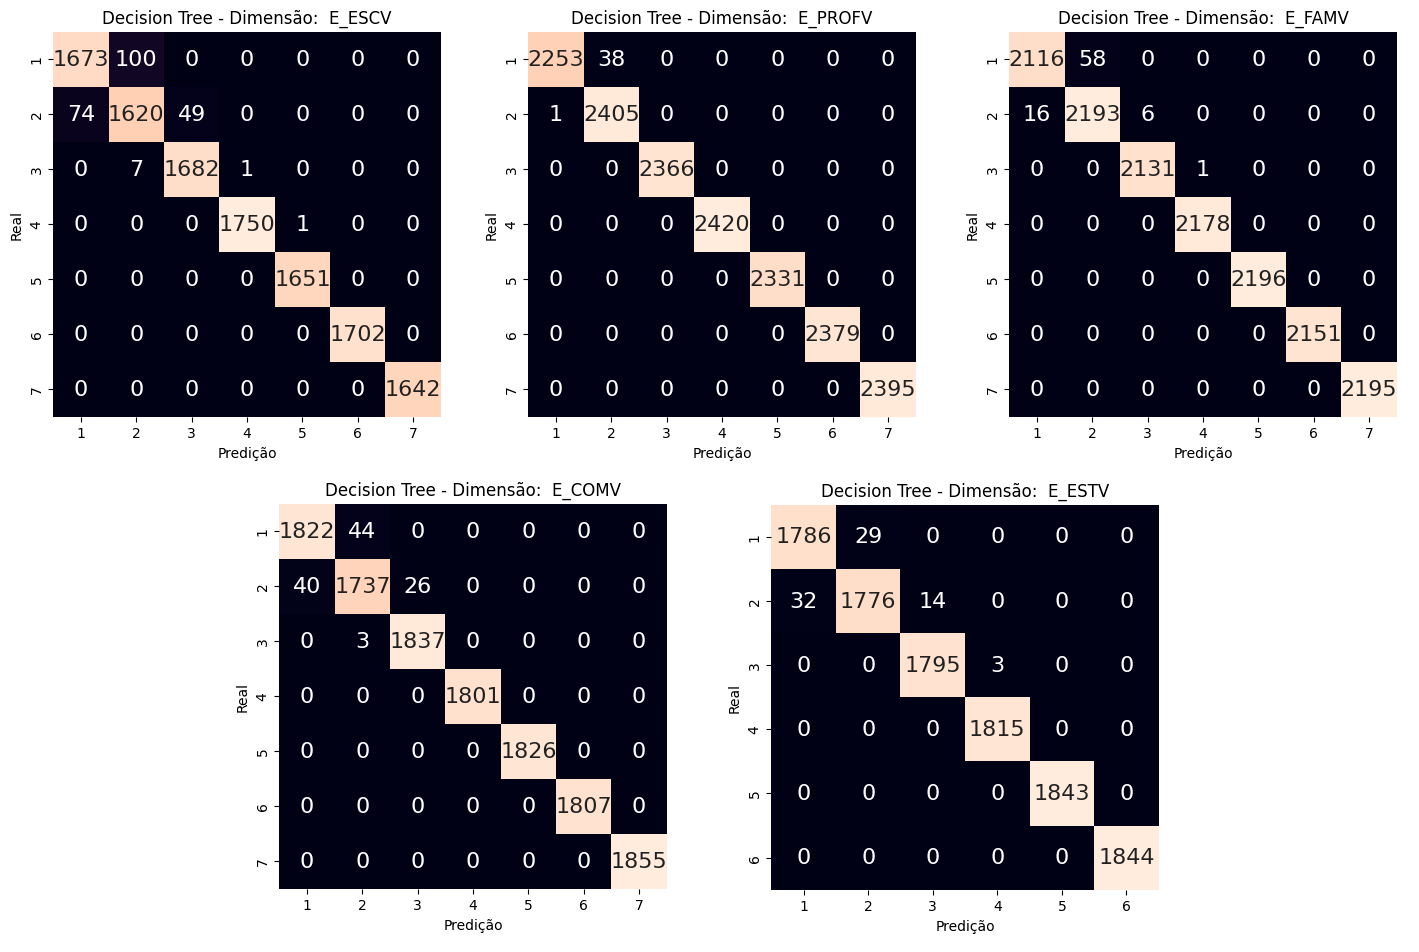
\includegraphics[width=0.8\textwidth]{Textuais/Imagens/Matriz Confusão/Dimensões/dim_dt.png}
    \caption{Matriz de Confusão das Dimensões - Modelo Decision Tree}
    \label{fig:matriz_confusao_dim_dt}
\end{figure}

\begin{figure}[ht]
    \centering
    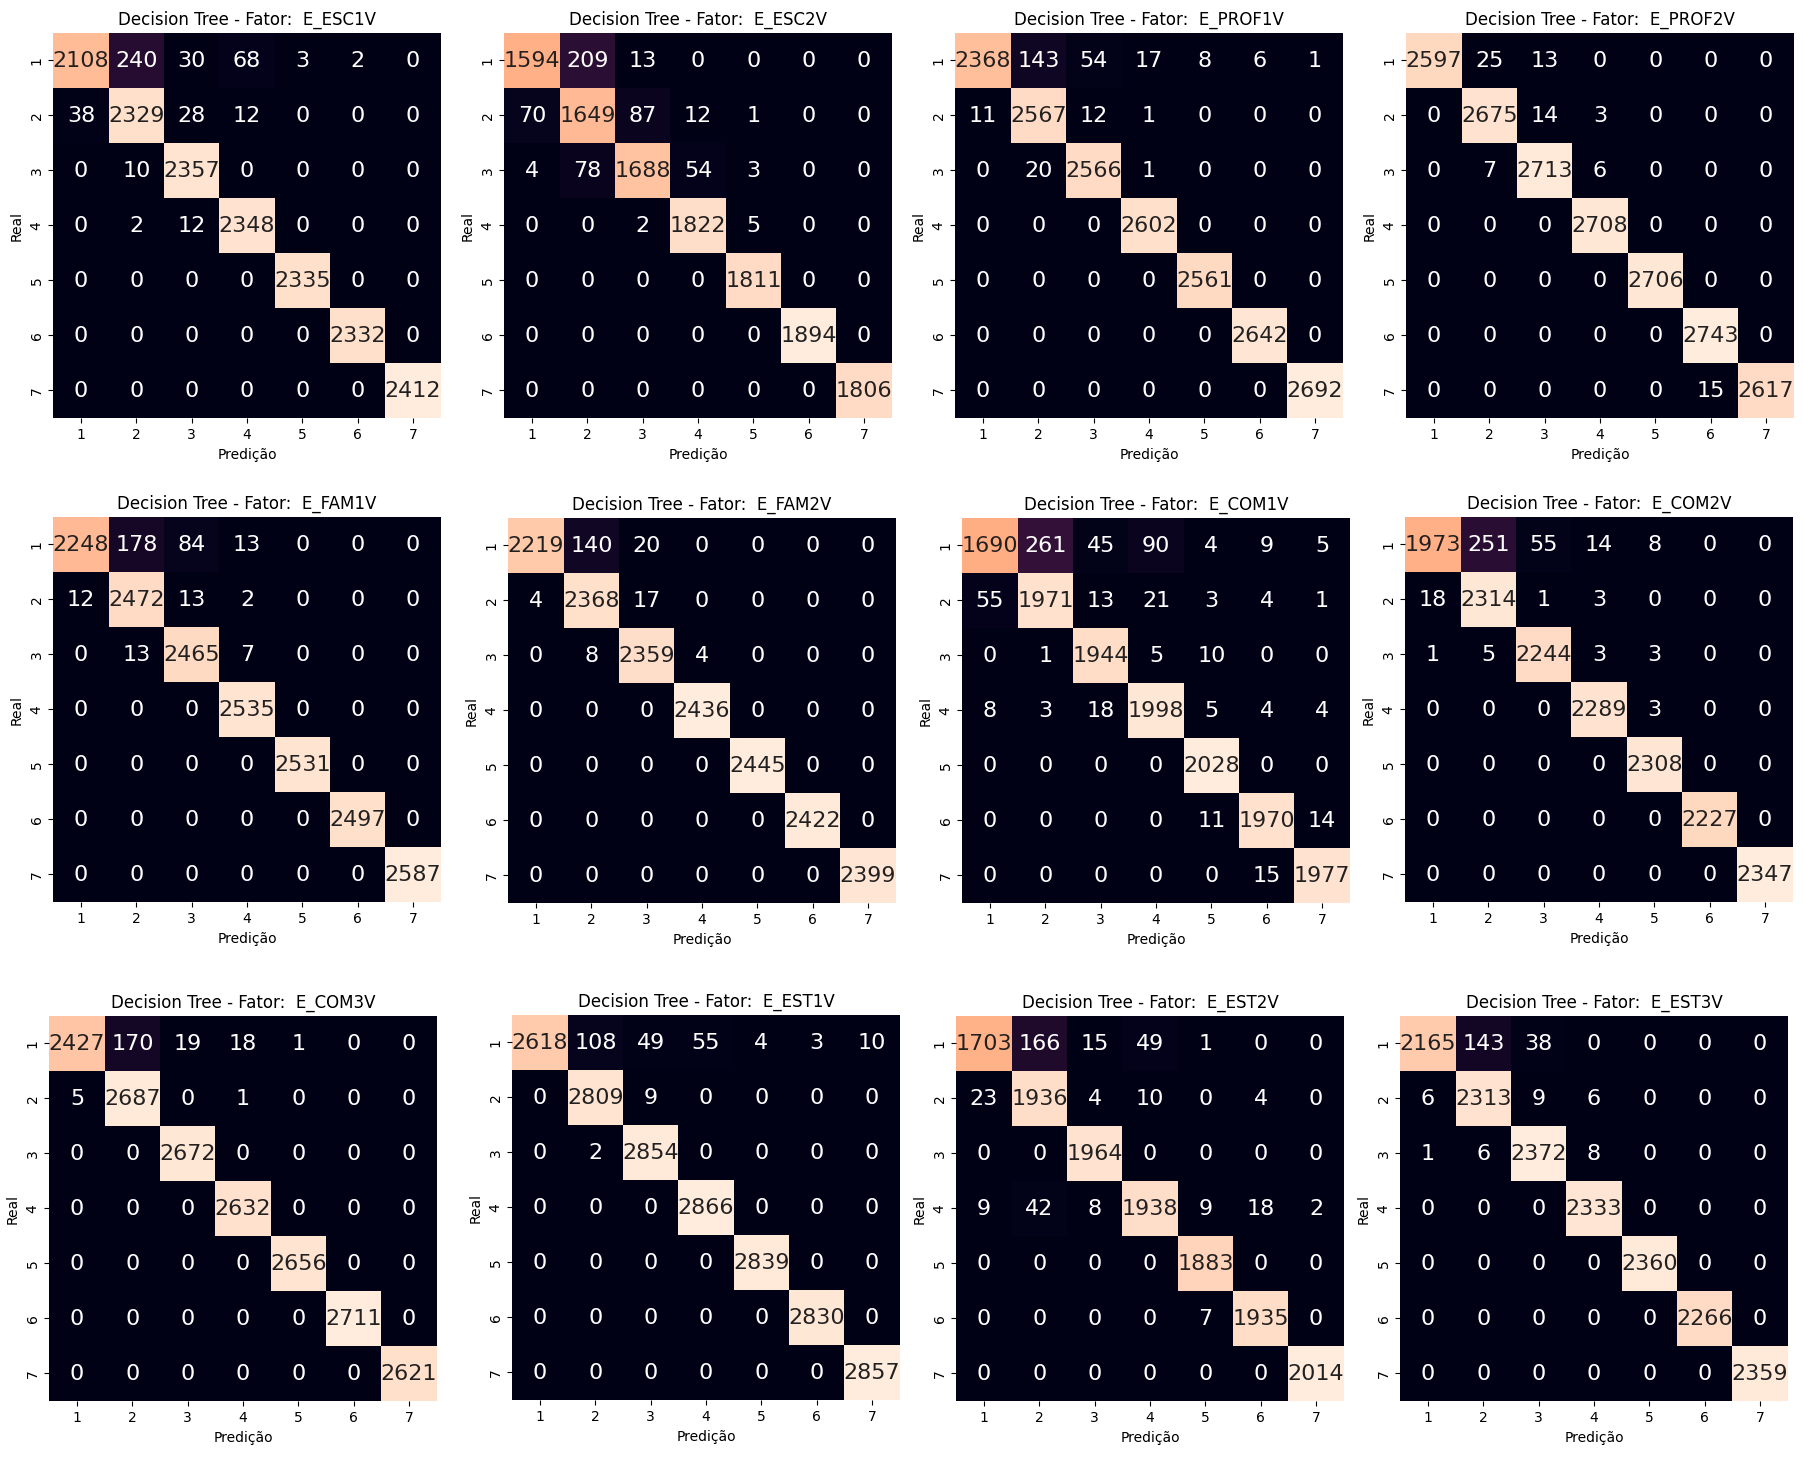
\includegraphics[width=0.8\textwidth]{Textuais/Imagens/Matriz Confusão/Fatores/DT.png}
    \caption{Matriz de Confusão dos Fatores - Modelo Decision Tree}
    \label{fig:matriz_confusao_fat_dt}
\end{figure}

% ----------------------------------------------------------
                      \chapter{Matrizes de confusão - Random Forest}
                      \label{ap2}
% ----------------------------------------------------------

\begin{figure}[ht]
    \centering
    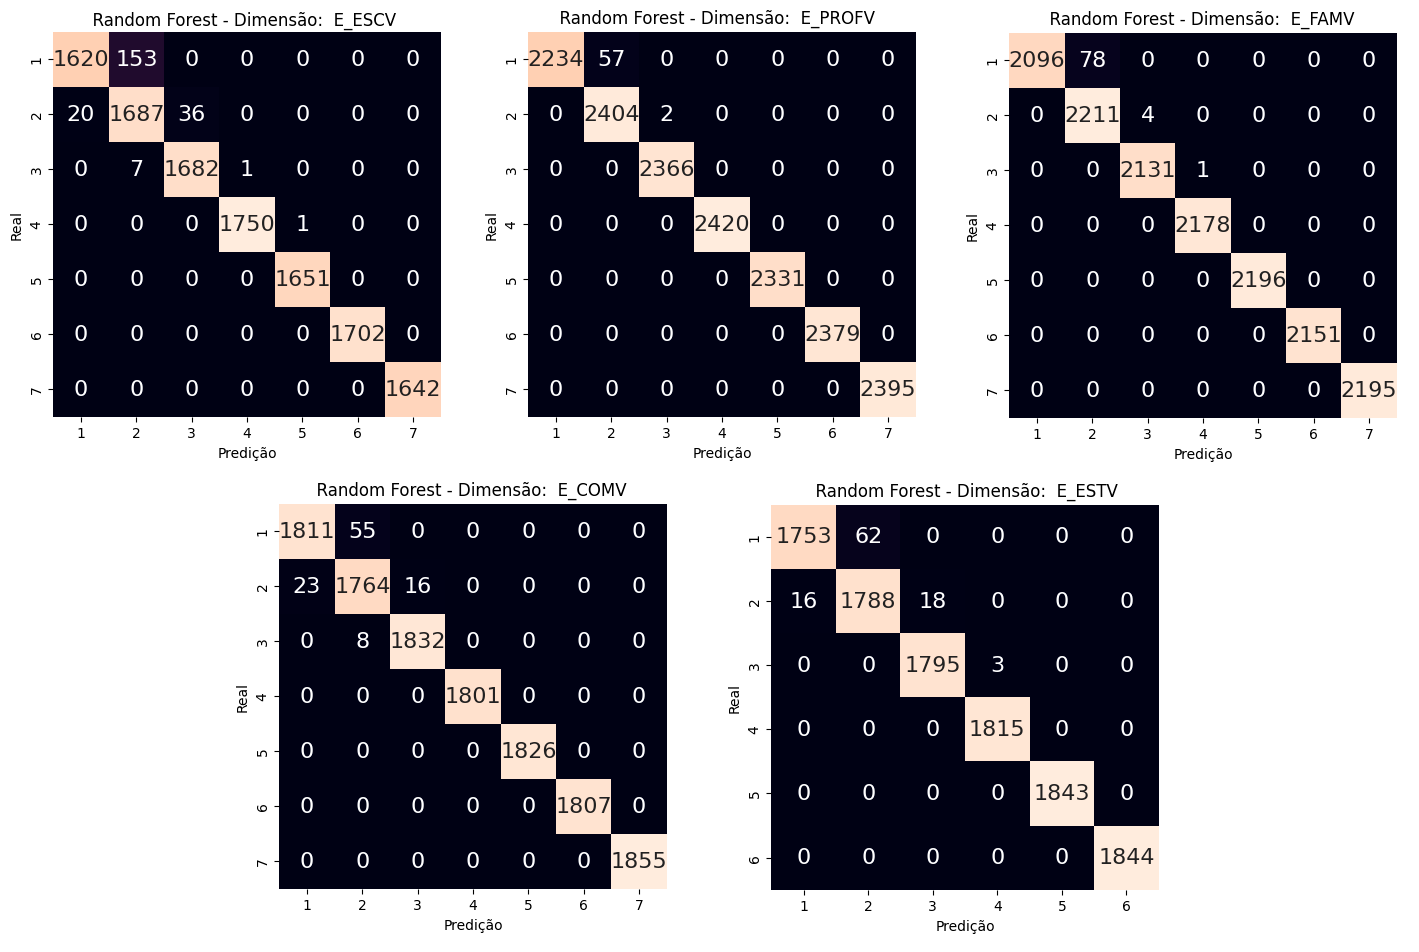
\includegraphics[width=0.8\textwidth]{Textuais/Imagens/Matriz Confusão/Dimensões/dim_rf.png}
    \caption{Matriz de Confusão das Dimensões - Modelo Random Forest}
    \label{fig:matriz_confusao_dim_rf}
\end{figure}

\begin{figure}[ht]
    \centering
    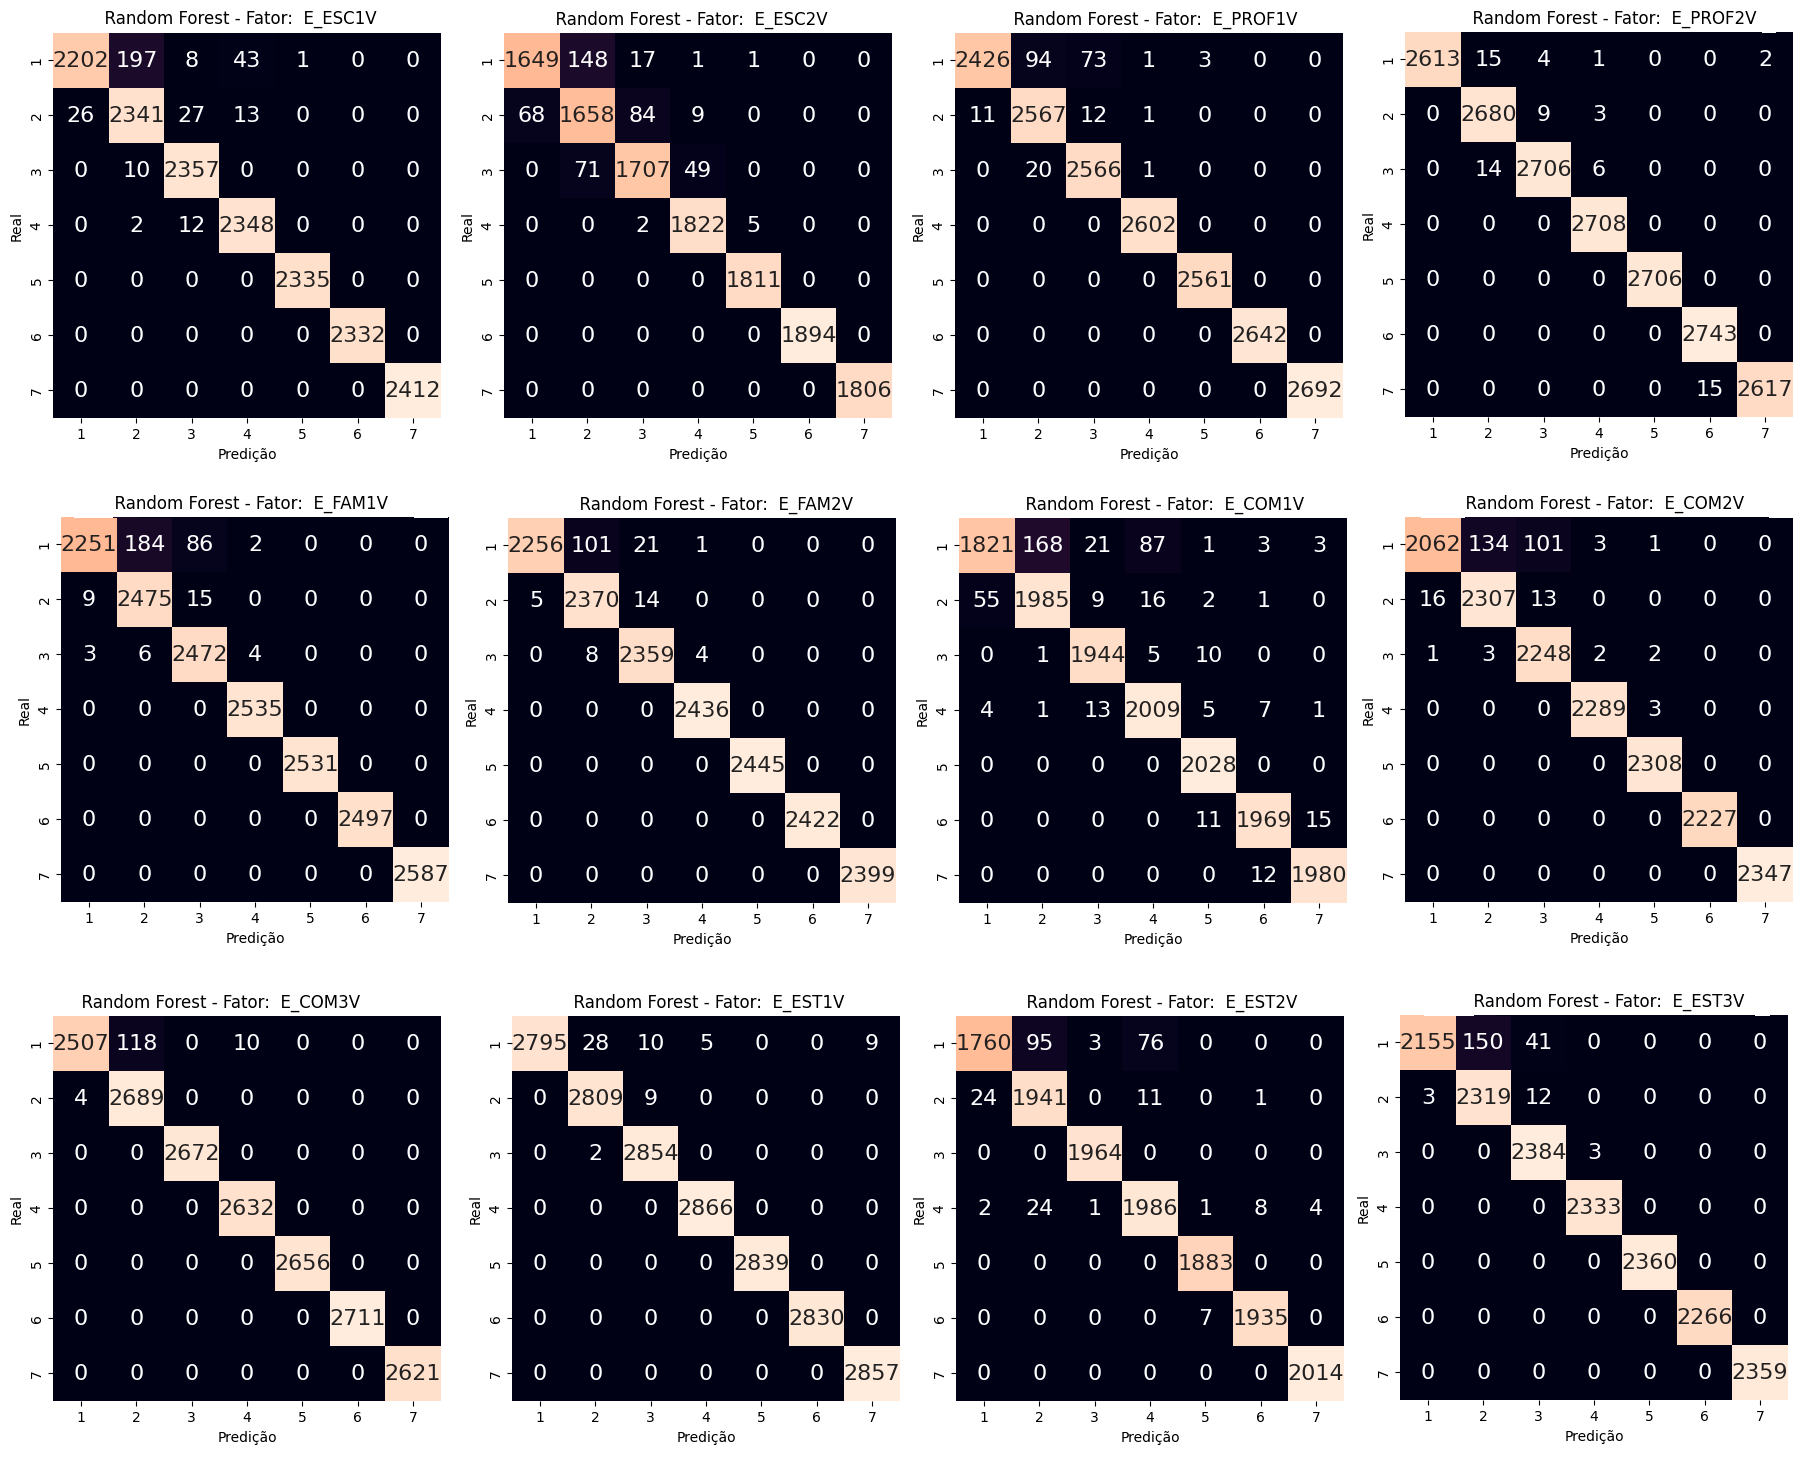
\includegraphics[width=0.8\textwidth]{Textuais/Imagens/Matriz Confusão/Fatores/RF.png}
    \caption{Matriz de Confusão dos Fatores - Modelo Random Forest}
    \label{fig:matriz_confusao_fat_rf}
\end{figure}

% ----------------------------------------------------------
                      \chapter{Matrizes de confusão - Modelo AdaBoost}
                      \label{ap3}
% ----------------------------------------------------------

\begin{figure}[ht]
    \centering
    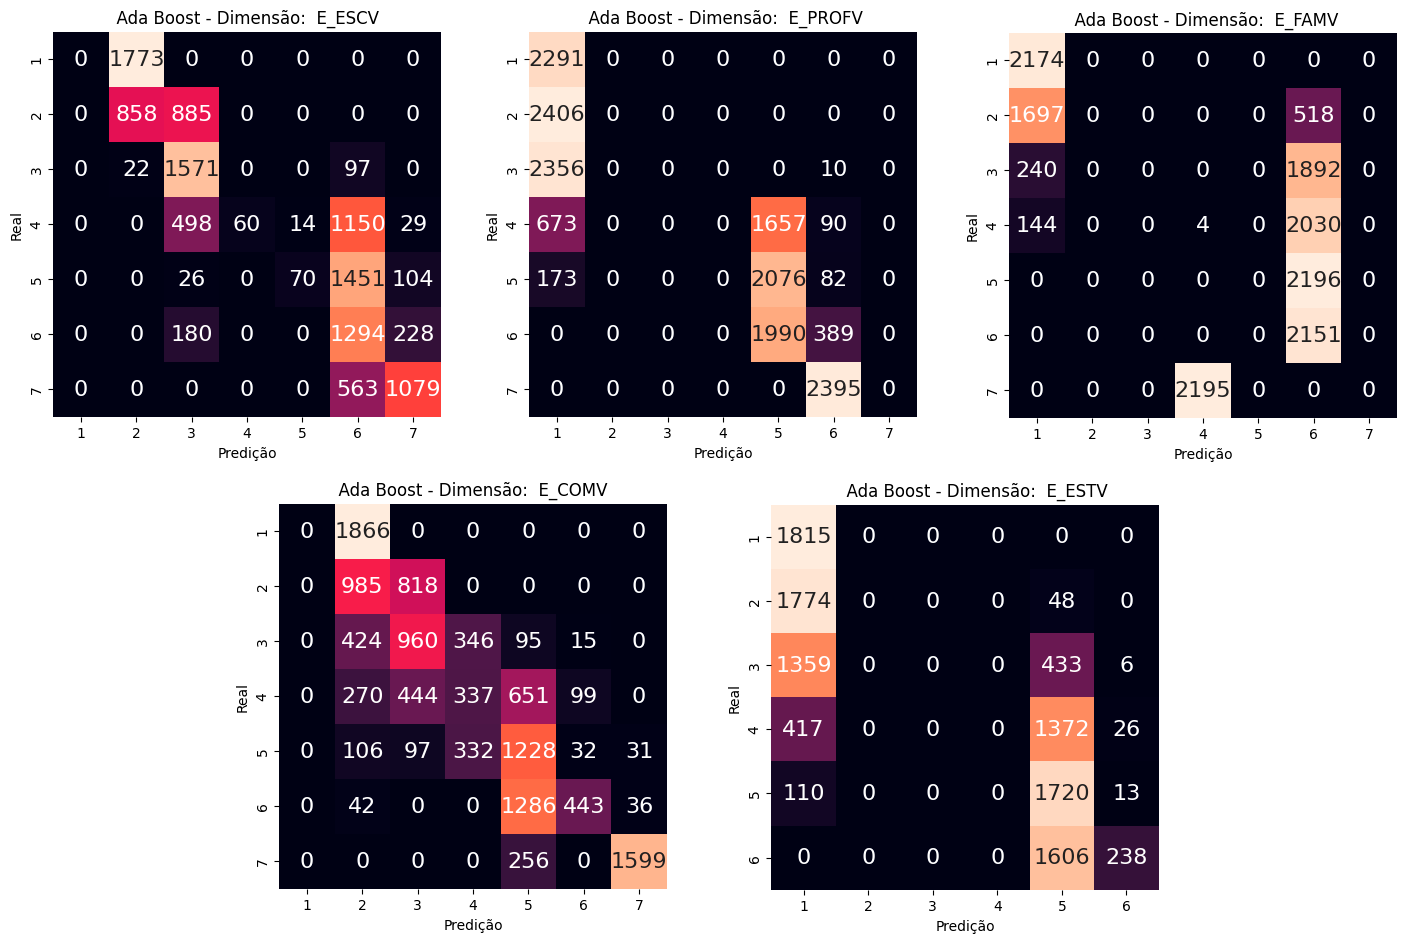
\includegraphics[width=0.8\textwidth]{Textuais/Imagens/Matriz Confusão/Dimensões/dim_ab.png}
    \caption{Matriz de Confusão das Dimensões - Modelo AdaBoost}
    \label{fig:matriz_confusao_dim_ab}
\end{figure}

\begin{figure}[ht]
    \centering
    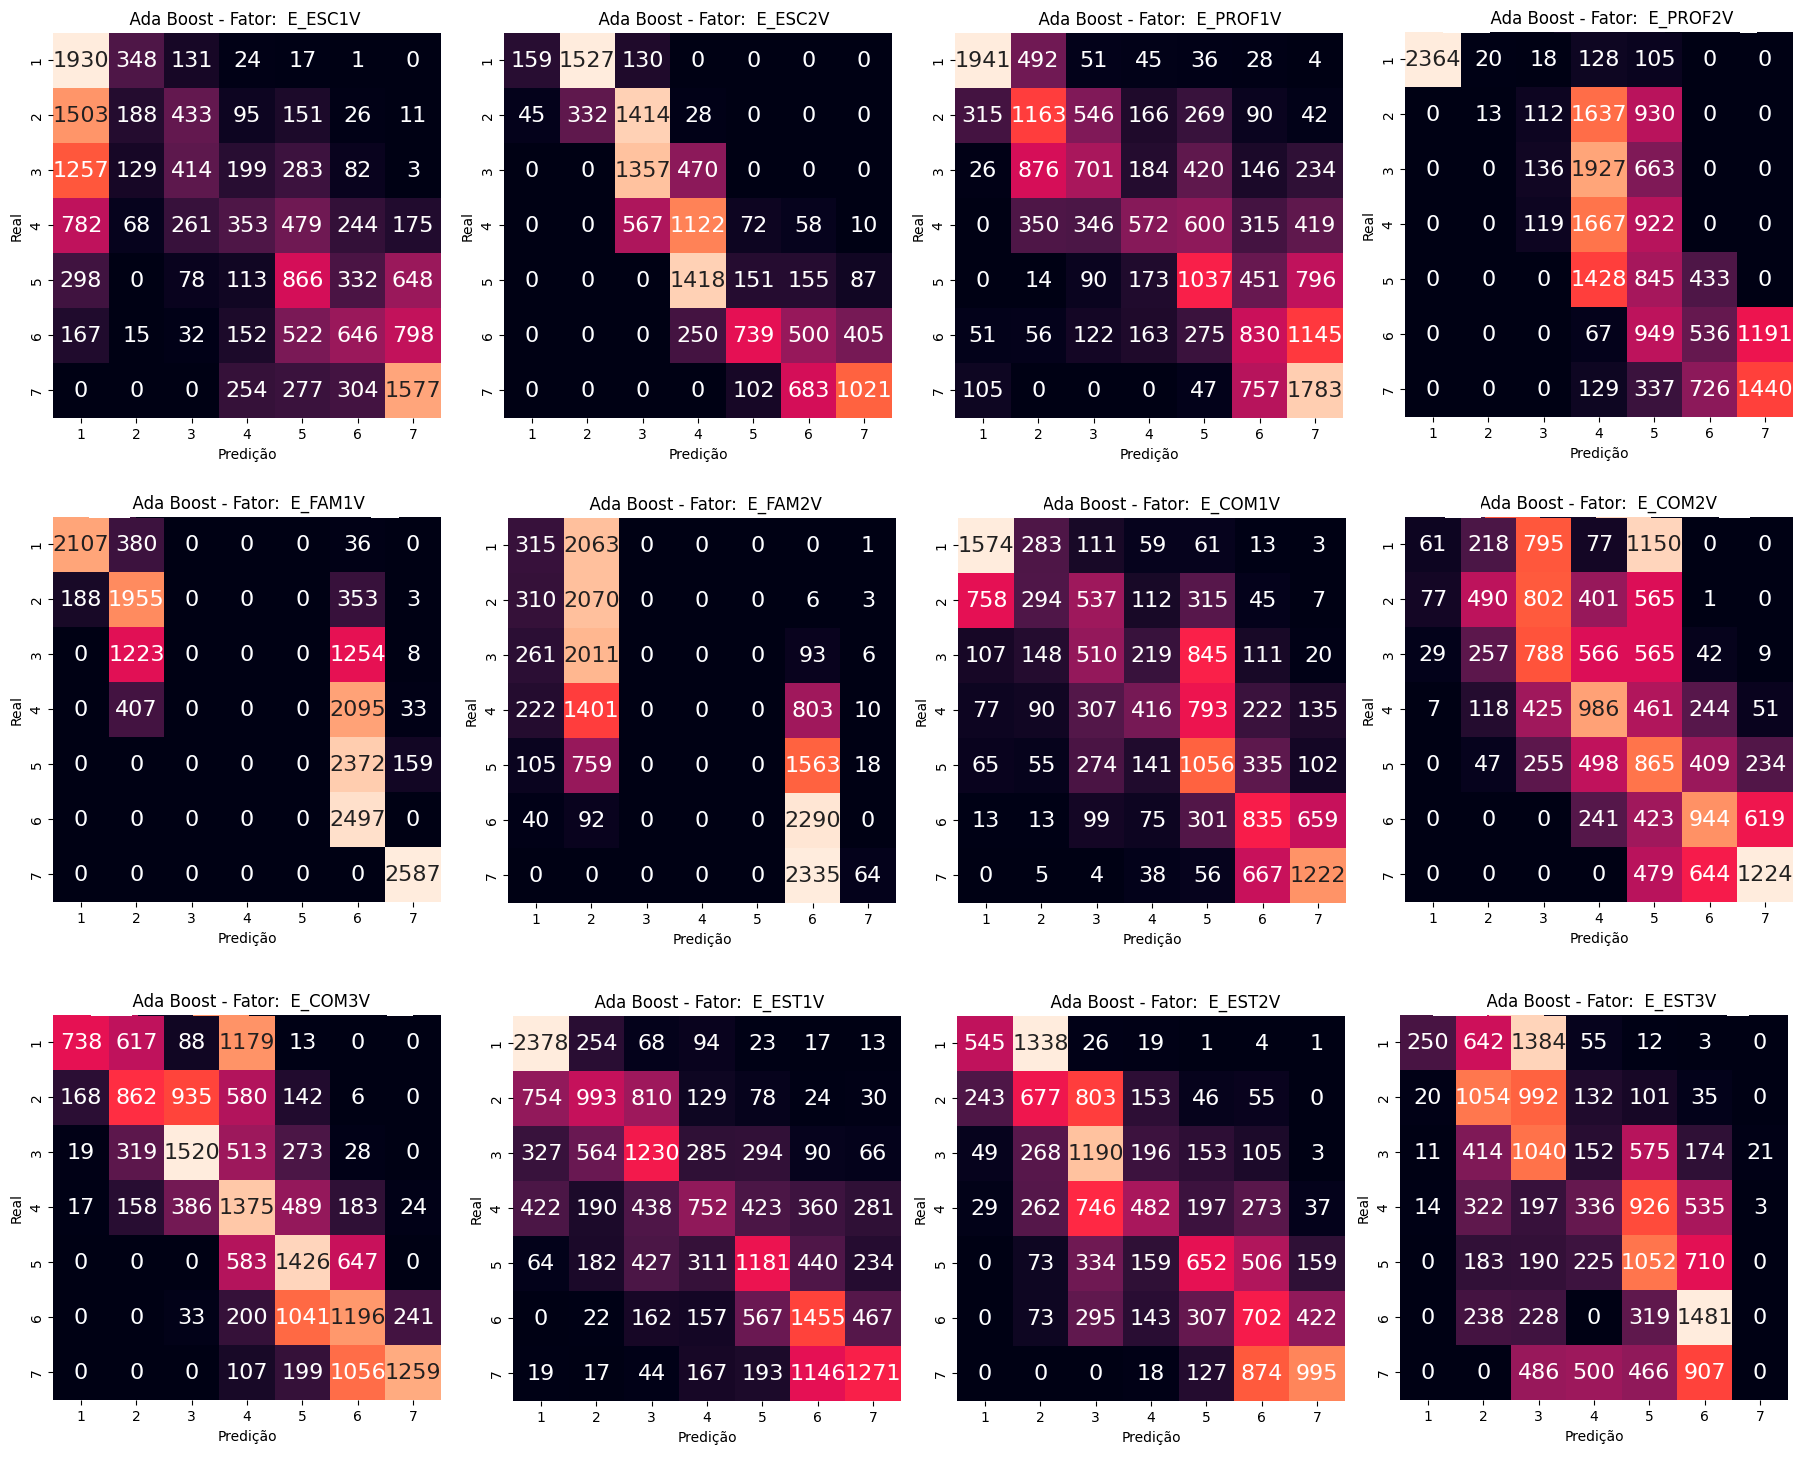
\includegraphics[width=0.8\textwidth]{Textuais/Imagens/Matriz Confusão/Fatores/AB.png}
    \caption{Matriz de Confusão dos Fatores - Modelo AdaBoost}
    \label{fig:matriz_confusao_fat_ab}
\end{figure}

% ----------------------------------------------------------
                      \chapter{Matrizes de confusão - Modelo Naive Bayes}
                      \label{ap4}
% ----------------------------------------------------------

\begin{figure}[ht]
    \centering
    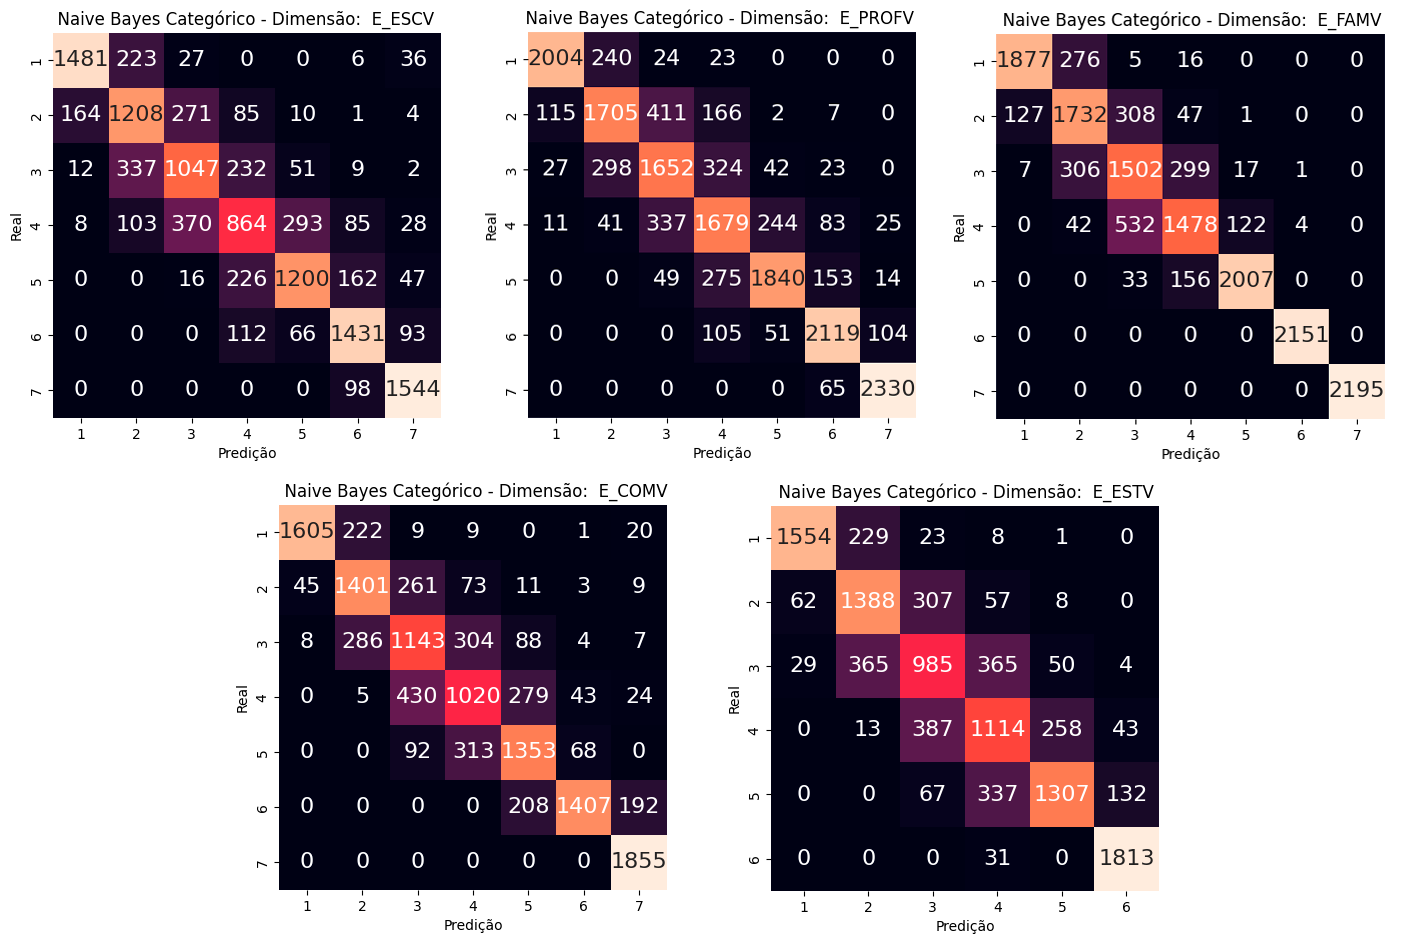
\includegraphics[width=0.8\textwidth]{Textuais/Imagens/Matriz Confusão/Dimensões/dim_nb.png}
    \caption{Matriz de Confusão das Dimensões - Modelo Naive Bayes}
    \label{fig:matriz_confusao_dim_nbc}
\end{figure}

\begin{figure}[ht]
    \centering
    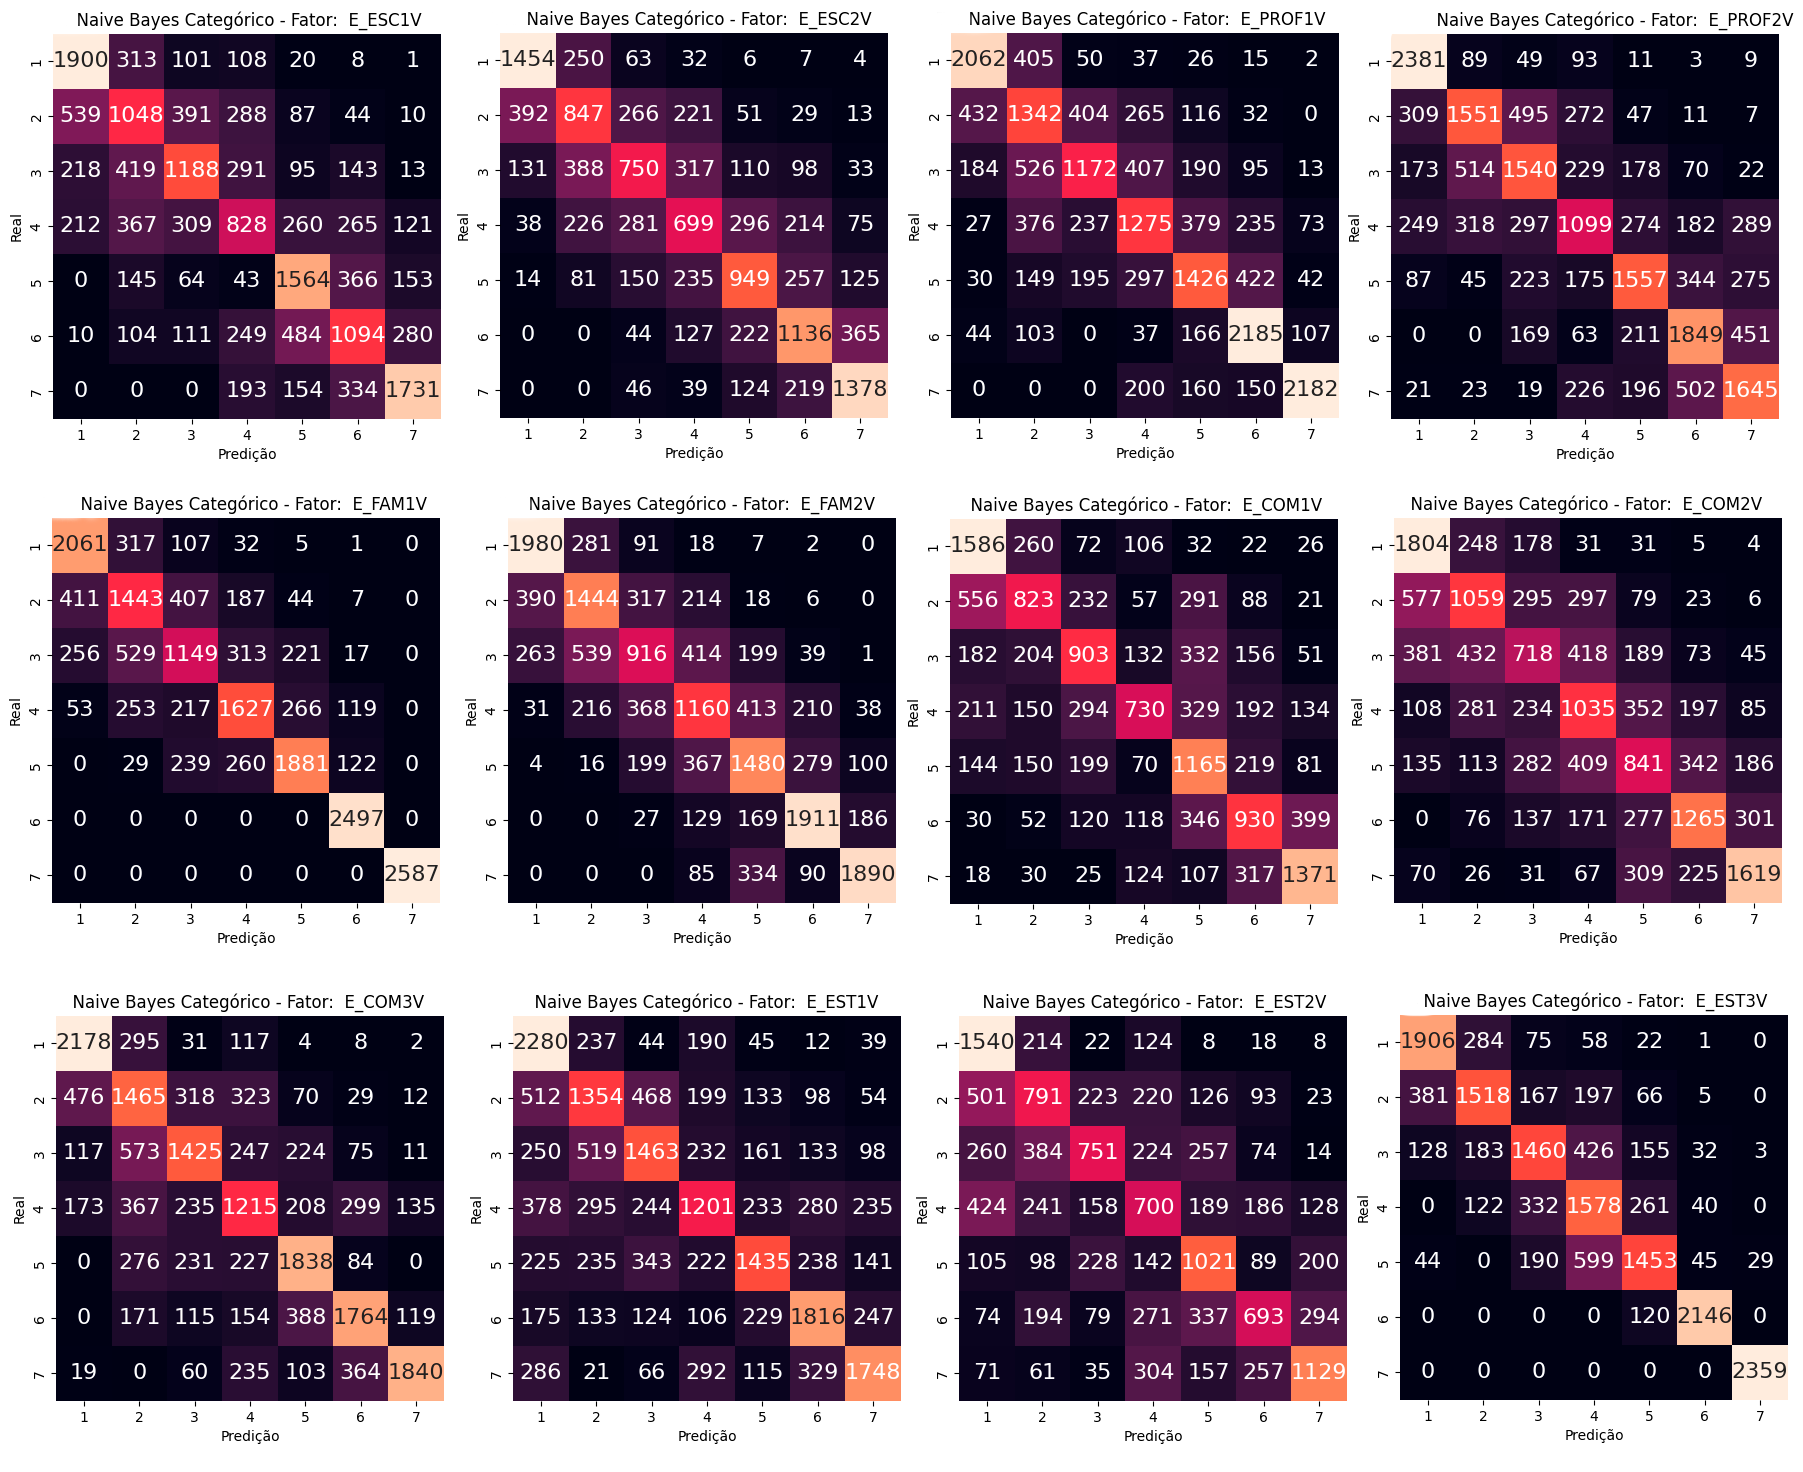
\includegraphics[width=0.8\textwidth]{Textuais/Imagens/Matriz Confusão/Fatores/NBC.png}
    \caption{Matriz de Confusão dos Fatores - Modelo Naive Bayes}
    \label{fig:matriz_confusao_fat_nbc}
\end{figure}

% ----------------------------------------------------------
                      \chapter{Matrizes de confusão - Modelo K Vizinhos Próximos}
                      \label{ap5}
% ----------------------------------------------------------

\begin{figure}[ht]
    \centering
    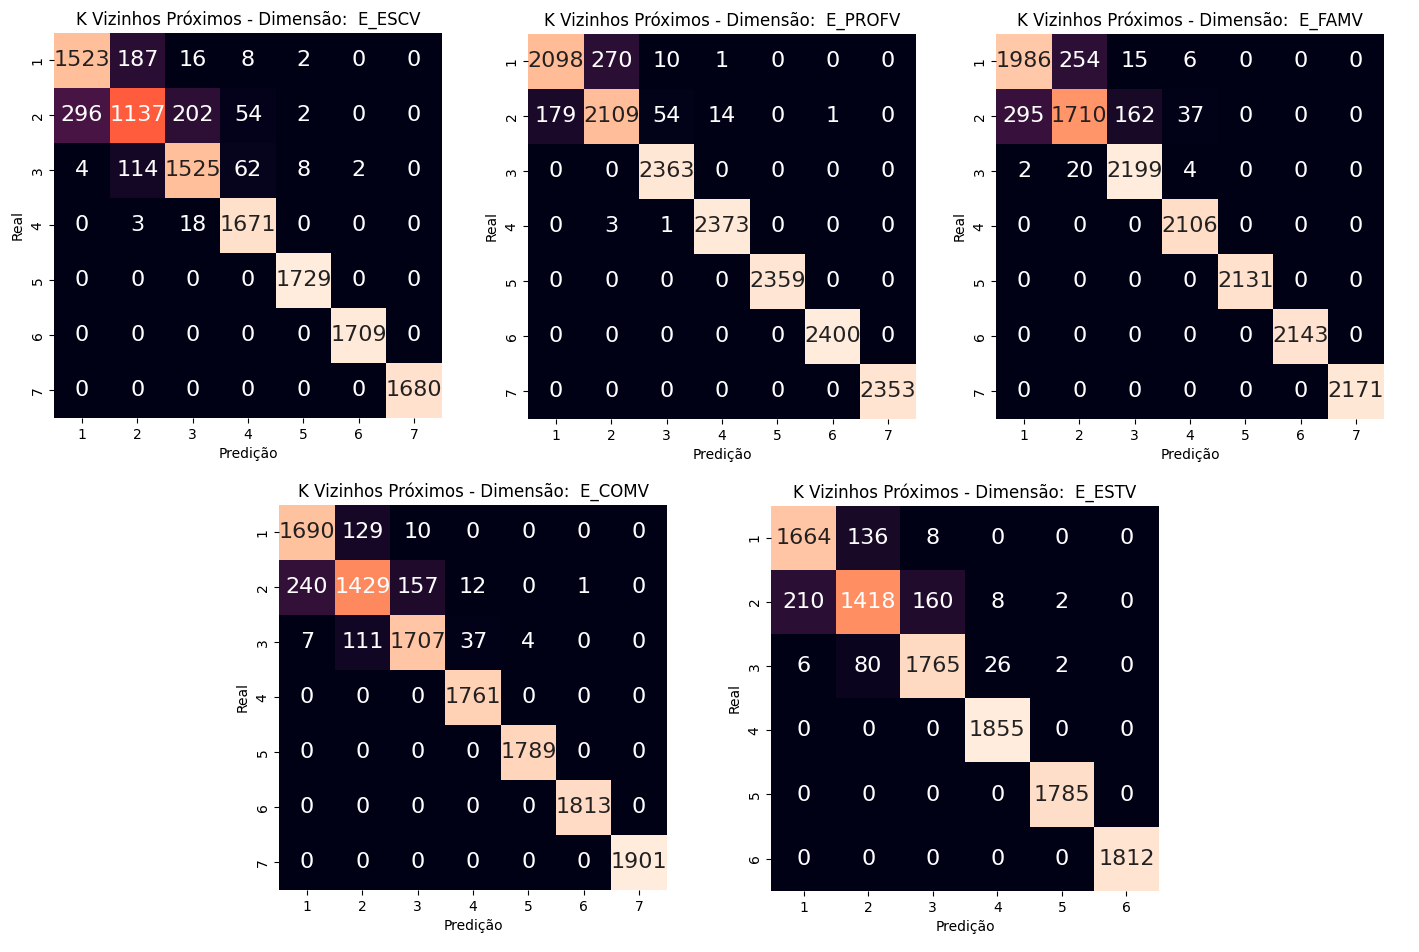
\includegraphics[width=0.8\textwidth]{Textuais/Imagens/Matriz Confusão/Dimensões/dim_knn.png}
    \caption{Matriz de Confusão das Dimensões - Modelo K Vizinhos Próximos}
    \label{fig:matriz_confusao_dim_knn}
\end{figure}

\begin{figure}[ht]
    \centering
    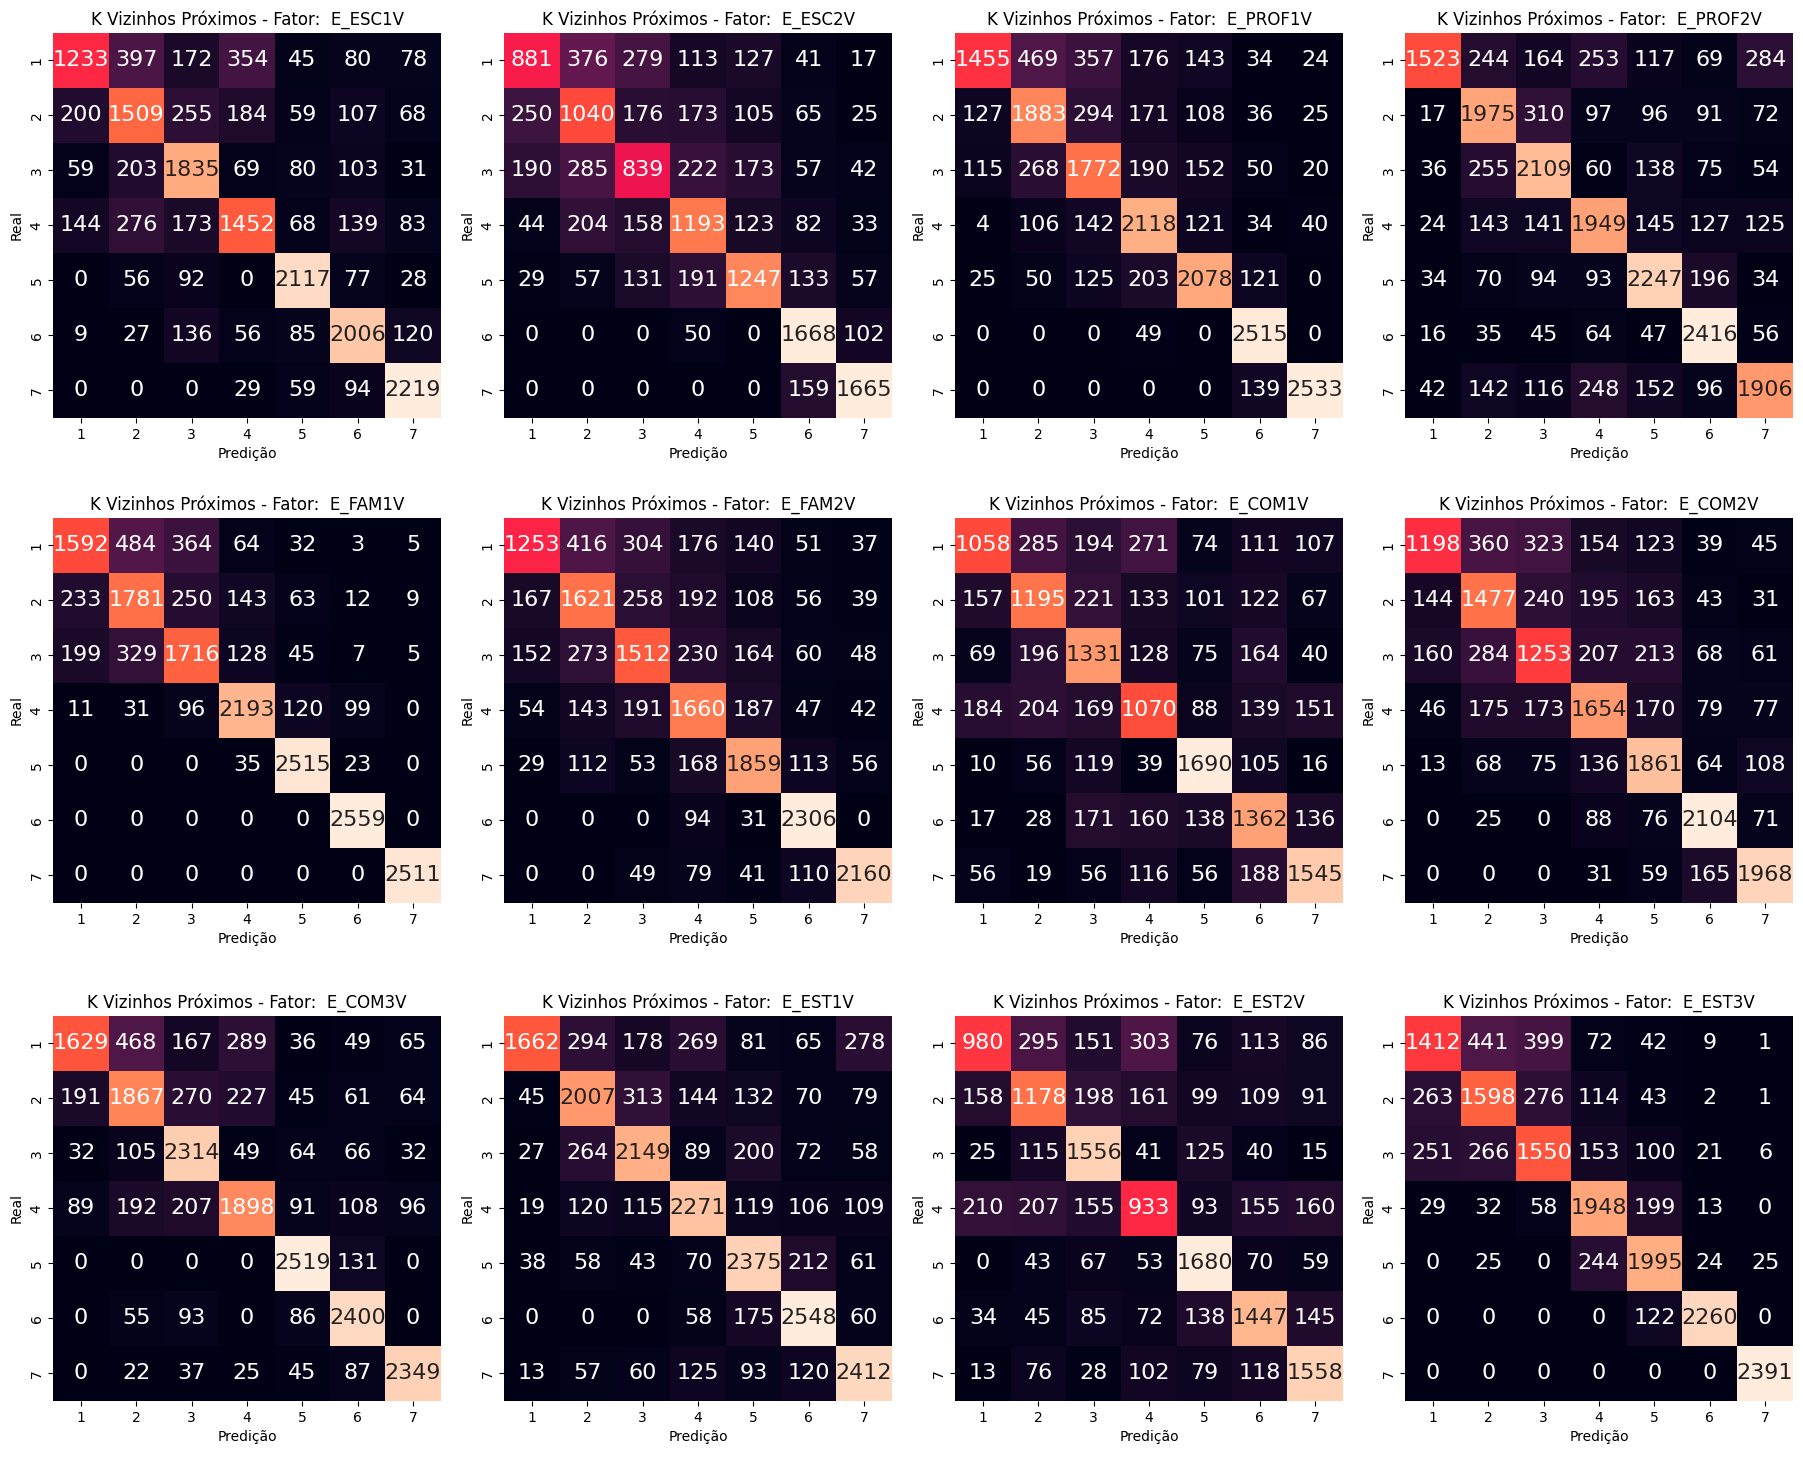
\includegraphics[width=0.8\textwidth]{Textuais/Imagens/Matriz Confusão/Fatores/KNN.png}
    \caption{Matriz de Confusão dos Fatores - Modelo K Vizinhos Próximos}
    \label{fig:matriz_confusao_fat_knn}
\end{figure}

                      \end{apendicesenv}
% ---				% Elemento Opcional

% % ----------------------------------------------------------
% % Anexos
% % ----------------------------------------------------------
% %
% % ---
% Inicia os anexos
% ---
\begin{anexosenv}

% Imprime uma página indicando o início dos anexos
\partanexos

% ---
% \chapter{IAFREE-R}
% ---

\includepdf[pages=-]{PosTextuais/organized-1-1.pdf}

\end{anexosenv}
				% Elemento Opcional

% %%---------------------------------------------------------------------
% %% INDICE REMISSIVO
% %%---------------------------------------------------------------------

% %\phantompart
% %\printindex

% %---------------------------------------------------------------------

% %%---------------------------------------------------------------------
% %% INDICE REMISSIVO (Formatado Manualmente)
% %%---------------------------------------------------------------------

% \chapter*{ÍNDICE}
% \addcontentsline{toc}{chapter}{ÍNDICE}

% { \setlength{\parindent}{0pt}  % ambiente sem indentação
	
% Andesito, 22, 50, 73

% Argila, 52, 75, 121

% Basalto, 25, 230, 235

	
	
	
	
% } % fim ambiente sem indentação


		% Elemento Opcional

\end{document}

% -----------------------------------------------------------------
% Fim do Documento
% -----------------------------------------------------------------	